%%
%% This is file `mcmthesis-demo.tex',
%% generated with the docstrip utility.
%%
%% The original source files were:
%%
%% mcmthesis.dtx  (with options: `demo')
%%
%% -----------------------------------
%%
%% This is a generated file.
%%
%% Copyright (C)
%%       2010 -- 2015 by Zhaoli Wang
%%       2014 -- 2019 by Liam Huang
%%       2019 -- present by latexstudio.net
%%
%% This work may be distributed and/or modified under the
%% conditions of the LaTeX Project Public License, either version 1.3
%% of this license or (at your option) any later version.
%% The latest version of this license is in
%%   http://www.latex-project.org/lppl.txt
%% and version 1.3 or later is part of all distributions of LaTeX
%% version 2005/12/01 or later.
%%
%% This work has the LPPL maintenance status `maintained'.
%%
%% The Current Maintainer of this work is Liam Huang.
%%
%%
%% This is file `mcmthesis-demo.tex',
%% generated with the docstrip utility.
%%
%% The original source files were:
%%
%% mcmthesis.dtx  (with options: `demo')
%%
%% -----------------------------------
%%
%% This is a generated file.
%%
%% Copyright (C)
%%       2010 -- 2015 by Zhaoli Wang
%%       2014 -- 2019 by Liam Huang
%%       2019 -- present by latexstudio.net
%%
%% This work may be distributed and/or modified under the
%% conditions of the LaTeX Project Public License, either version 1.3
%% of this license or (at your option) any later version.
%% The latest version of this license is in
%%   http://www.latex-project.org/lppl.txt
%% and version 1.3 or later is part of all distributions of LaTeX
%% version 2005/12/01 or later.
%%
%% This work has the LPPL maintenance status `maintained'.
%%
%% The Current Maintainer of this work is Liam Huang.
%%
\documentclass{mcmthesis}
\mcmsetup{CTeX = false,    % 使用 CTeX 套装时,设置为 true
          tcn = {2519530}, problem = \textcolor{red}{C},
          sheet = true, titleinsheet = true, keywordsinsheet = true,
          titlepage = false, abstract = false}
        
\usepackage{newtxtext}     % \usepackage{palatino}
\usepackage[options]{algorithm2e}
\usepackage[backend=bibtex]{biblatex}   % for RStudio Complie

\usepackage{amsmath}
\usepackage{hyperref}
\usepackage[ruled,vlined]{algorithm2e}

\usepackage{tocloft}
\setlength{\cftbeforesecskip}{6pt}
\renewcommand{\contentsname}{\hspace*{\fill}\Large\bfseries Contents \hspace*{\fill}}
\usepackage{subcaption}

\title{GAMMA Fusion: A \underline{G}eneralized \underline{A}thelete \underline{M}odel for \underline{M}edal \underline{A}nalysis based on Gamma Function}
% \author{\small \href{http://www.latexstudio.net/}
%   {
\includegraphics[width=7cm]{mcmthesis-logo}}}
\date{\today}
\begin{document}
\begin{abstract}

Predicting the medal counts table at the 2028 Olympic Games is no doubt an intriguing topic. This paper introduces a GAMMA Fusion, which is comprised of a \textbf{Core Medal Prediction Model} patched by other impact factors, in order to provide better predictions. 

\textit{First}, we designed our model as an \textbf{integrated macro-micro model}, based on the \textbf{Gamma Model} we built for each (athlete, event) to show the strength change over time. We used \textbf{Least Square Method} to fit them into the model, with a final average loss of \textbf{0.7557}. We also built a \textbf{Country / Sport Gamma Model} concluded from individual ones, dynamically changing over time. 

\textit{Next}, we constructed \textbf{Core Medal Prediction Model} based on the models above, separating countries into two layers. In the first layer, elite countries' athletes were divided into \textbf{recruits} (new athlete) and \textbf{veterans} (old athletes). For recruits, we utilized \textbf{EWMA} recruits number prediction and Country/Sport Gamma Models patching. For veterans, we adopted \textbf{Logistic Regression} for dropout rate and \textbf{Bayesian Inference} for revision. We used these results to predict preliminary 2028 model counts. We got \textbf{Prediction Intervals} by adopting \textbf{Monte-Carlo Simulation}. In the second layer, we grouped unexceptional countries and considered both random effect and stable improvement, using \textbf{ARIMA} and the Gamma Model respectively.
%\textit{Next}, we constructed our \textbf{Core Medal Prediction Model} based on the models above, separating countries into two layers. In the \textbf{first layer}, elite countries are treated separately. We continued to divided athletes into two categories: \textbf{recruits} (new athlete) and \textbf{veterans} (old athletes). For recruits, we utilized \textbf{EWMA} to predict the number of recruits and another EWMA to predict and patch Country / Sport Gamma Models after analyzing model credibility. For veterans, we adopted \textbf{Logistic Regression} to get a dropout rate and \textbf{Bayesian Inference} to revise their Gamma models. We used these results to predict preliminary 2028 model counts. Since we're sampling data from distributions, we can easily get \textbf{Prediction Intervals} by adopting \textbf{Monte-Carlo Simulation}. In the \textbf{second layer}, we grouped unexceptional countries together and considered both random effect and stable improvement, using \textbf{ARIMA} and the Gamma Model respectively.
%--一半--


\textit{Then}, we used \textbf{Principal Component Analysis (PCA)} model to take sports advantage into further account. First, the data-set is down-scaled through \textbf{Pearson Correlation Coefficient} and \textbf{ReLU} process, and the General Advantage is analyzed with PCA, gathering similar sports and unveiling countries' important sports. Second, Home Country Effect (HCE) is analysed with simple \textbf{regression equation fitting}, and \textbf{features (Hierarchy, the Trailing Effect)} is summarized, offering a general 16.7\% boost in the number of medals.

\textit{Besides}, Great Coach Effect (GCE) is brought out to complete our model. We first employed \textbf{time-series differencing method}, sorting out the possible evidence and comparing to historical fact, where coaches were \textbf{divided into world class and national greatness}. This method achieved a remarkable \textbf{65\%} accuracy. Then we estimated the impact and added other factors like \textbf{outcomes and costs} to the model, refining its performance. Finally, suggestions were given to \textbf{Canada, New Zealand, Australia} to take advantage of GCE after employing our model.

\textit{Moreover}, this paper extends its analysis to other factors found during the model refining and outliers analysing process. Based on data facts, we explore and explained effects including \textbf{Monopoly of Big Countries, Sudden Injuries, Geographical Differences, and Further HCE}, and finally offered some suggestions to the Olympic Committee, in order to further the \textbf{JUSTICE criterion}.

\textit{Finally}, we used the patched model to predict 2028 medal distribution, giving USA, CHN, GBR, JPN, KOR to be top 5. Our model achieved 86.67\% stability in maintaining classification, and have 82\% similarity with historical American host Olympics data. 

%注意时态
%确保格式一致
%写notations
%注意前后文中文注释
%文中[EnglishDescription]改写为notations
%大小写
%加粗问题
%所有的Fig.的引用\ref{}改写,补上

\begin{keywords}
Olympics medal prediction, Gamma distribution, Bayesian inference, EWMA, Time Series Analysis, PCA, Monte Carlo Simulation
\end{keywords}

\end{abstract}

\maketitle


%% Generate the Table of Contents, if it's needed.
% \renewcommand{\contentsname}{\centering Contents}
\tableofcontents
\thispagestyle{empty}

\newpage

\section{Introduction}

%\subsection{Background}

The 2024 Paris Olympic Games saw the United States top the medal count with 126 total medals, tying with China for the most gold medals (40 each). France, the host country, ranked $5^{th}$ in gold medals and $4^{th}$ in total medals, while Great Britain ranked $7^{th}$ in gold medals and $3^{rd}$ in total medals. In addition to the medal results that have captured much attention, there are also some equally noteworthy outcomes. Countries like Albania, Cabo Verde, Dominica, and Saint Lucia won their first Olympic medals. We are interested in the probability of the occurrence of both these two cases.

We need to develop a model to predict medal counts for the 2028 Los Angeles Olympics, including prediction intervals and comparisons of medal situations before and after. In addition, we are tasked with predicting first-time medal winning countries and analysing the relationship between events and medal counts, while exploring the influence of Home Country preferences on event selection. Next, we'll assess the impact of 'great coaches' on performance and provide recommendations for investment in coaching for three countries. Finally, additional findings based on the model will be presented.

\begin{figure}
    \centering
    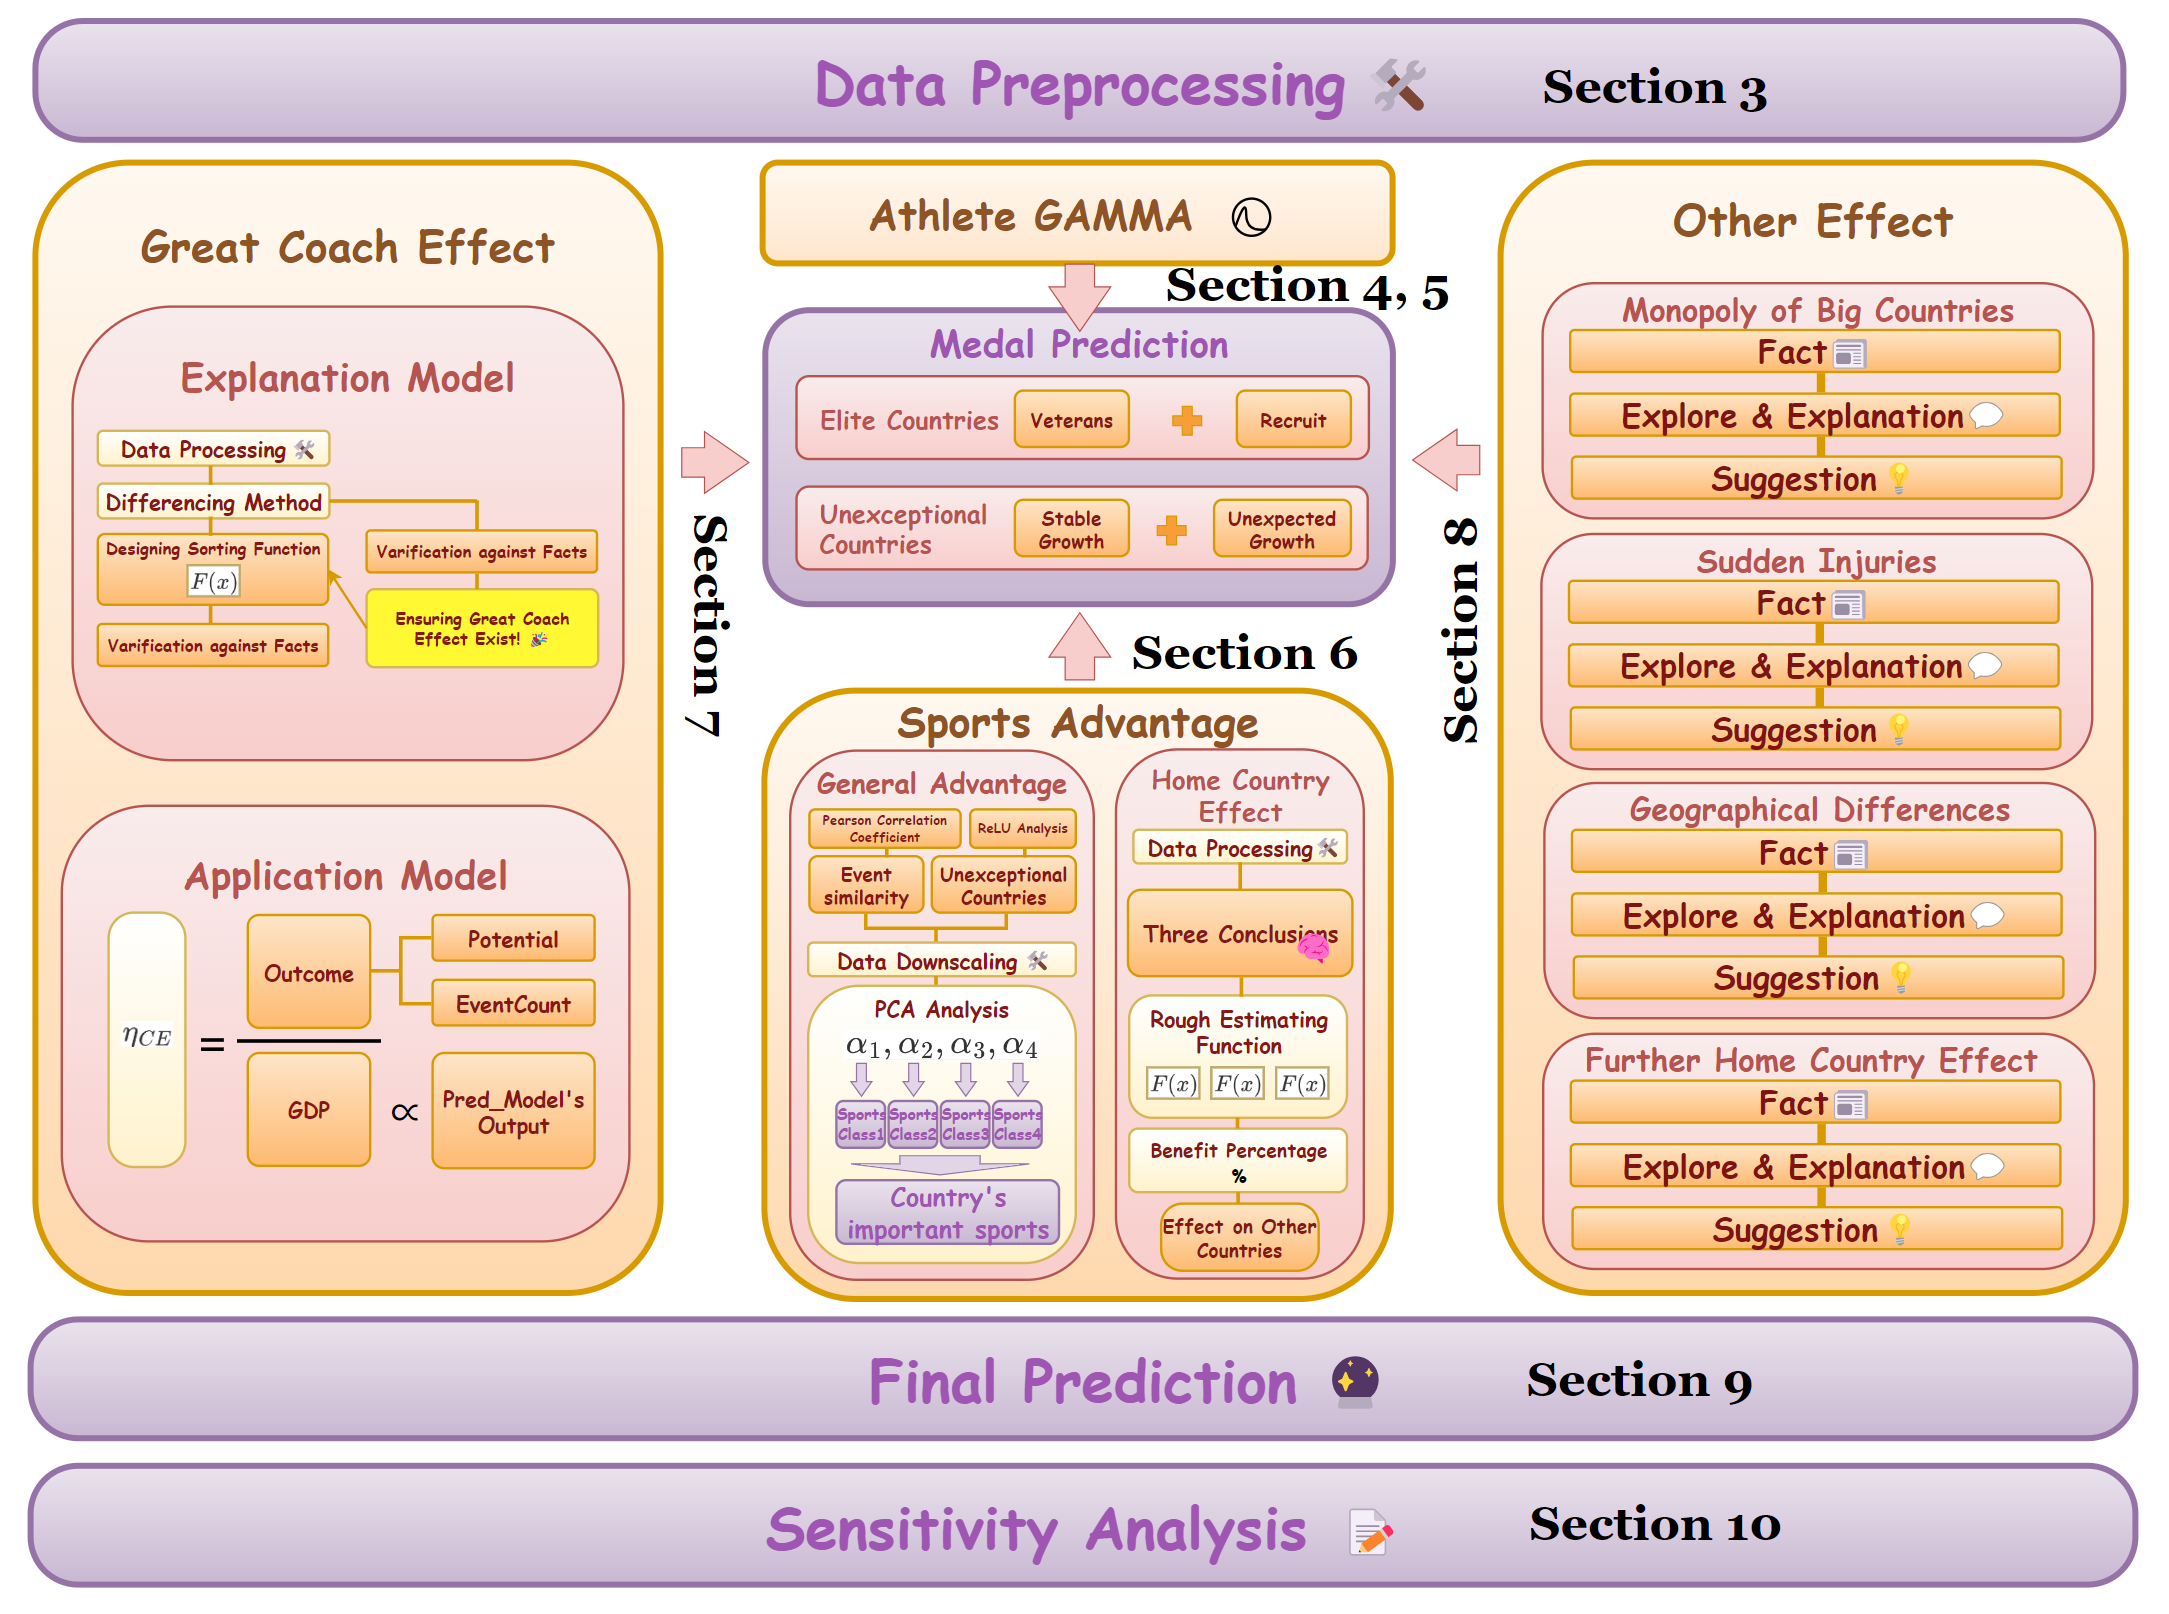
\includegraphics[width=1\linewidth]{Workflow.png}
    \caption{Overall Workflow}
    \label{fig:enter-label}
\end{figure}

Our whole project is carried out in four steps: \textbf{Data processing}, \textbf{Model construction}, \textbf{Final prediction}, \textbf{Sensitivity analysis}. The Model construction step is the core of our project. We first created a rough and general model in Section 4 and 5. Then in Section 6, 7, and 8, we made use of the outliers from our model, explored the factors affecting the outliers, and build patches according to the different factors like Sports advantage, Great Coach Effect, etc. to refine our models. It was after we had built the model that we gave out our final prediction, examining our project's power.


\section{Assumptions and Notations}

\subsection{Assumptions}

To clarify the problem and facilitate model construction, the following assumptions are made:

\begin{itemize}
\item {\bf Each athlete-event pair and its intrinsic data can be treated as an independent unit}. We assume that the performance of athletes in different events does not influence each other as the external factors occurring between competitions tend to nullify the influences.

\item  {\bf Medal Weight}. We have a projection from Medal to weights, showing the importance and difficulty of different medals. 

\item  {\bf The strength of the athletes directly affect the medals they get}. Since there is little data, it is reasonable to make such an assumption, which discards other factors causing big fluctuations.

\item  {\bf Issues about dropping-one-year athlete} To simplify the model, we see athletes who attended 2020's Game, missed 2024's Game, but participated in 2028's Game as newcomers.

\end{itemize}

\subsection{Notations}
\begin{center}
\begin{tabular}{clc}
{\bf Symbols and Abbr.} & {\bf Description} \\[0.25cm]
$HC$ & Home Country \\[0.2cm]
$age$ & Representing the number of times athletes participated in the Olympics. \\[0.2cm]
$score$ & $\omega_{Gold} \cdot x_{Gold} + \omega_{Silver} \cdot x_{Silver} + \omega_{Bronze} \cdot x_{Bronze} + \omega_{NoMedal} \cdot x_{NoMedal}$ \\[0.2cm]
$\alpha_i$ & The i\_th eigenvector in descending order of eigenvalue \\[0.2cm]
$n_x$ & The medal number. x is the name of the medal. \\[0.2cm]
$\omega_x$ & The medal weight. x is the name of the medal. \\[0.2cm]
$\lambda_x$ & The coefficient before the function of x. x is any independent variable.
\end{tabular}
\end{center}
%有待补充


\section{Data Preprocessing}

\subsection{Data Initialization}
We based our study on the data from International Olympic Committee (IOC) 's website\cite{1}. Firstly, we analyzed and amended the four datasets. The amendments we made are listed below.
\begin{itemize}
\item {\texttt{summerOly\_programs.csv}}: We replaced all nonsense cells and empty cells with 0. We also renamed the sports in accordance with the \texttt{summerOly\_athletes.csv}, incorporate similar disciplines such as Rugby Union and Rugby Sevens.
\item {\texttt{summerOly\_athletes.csv}}: We removed entirely duplicate data, replaced all invalid entries, and weighted medals based on individual and team events to facilitate subsequent calculations of the actual medal count. We removed data before 1972, considering that due to complicated reasons (such as WWII, collapse of the Soviet Union), the early data hardly have any rule. We also integrated the data from West Germany with that from East Germany.
\end{itemize}

\subsection{Data Overview}


\begin{figure}[h!]
    \centering
    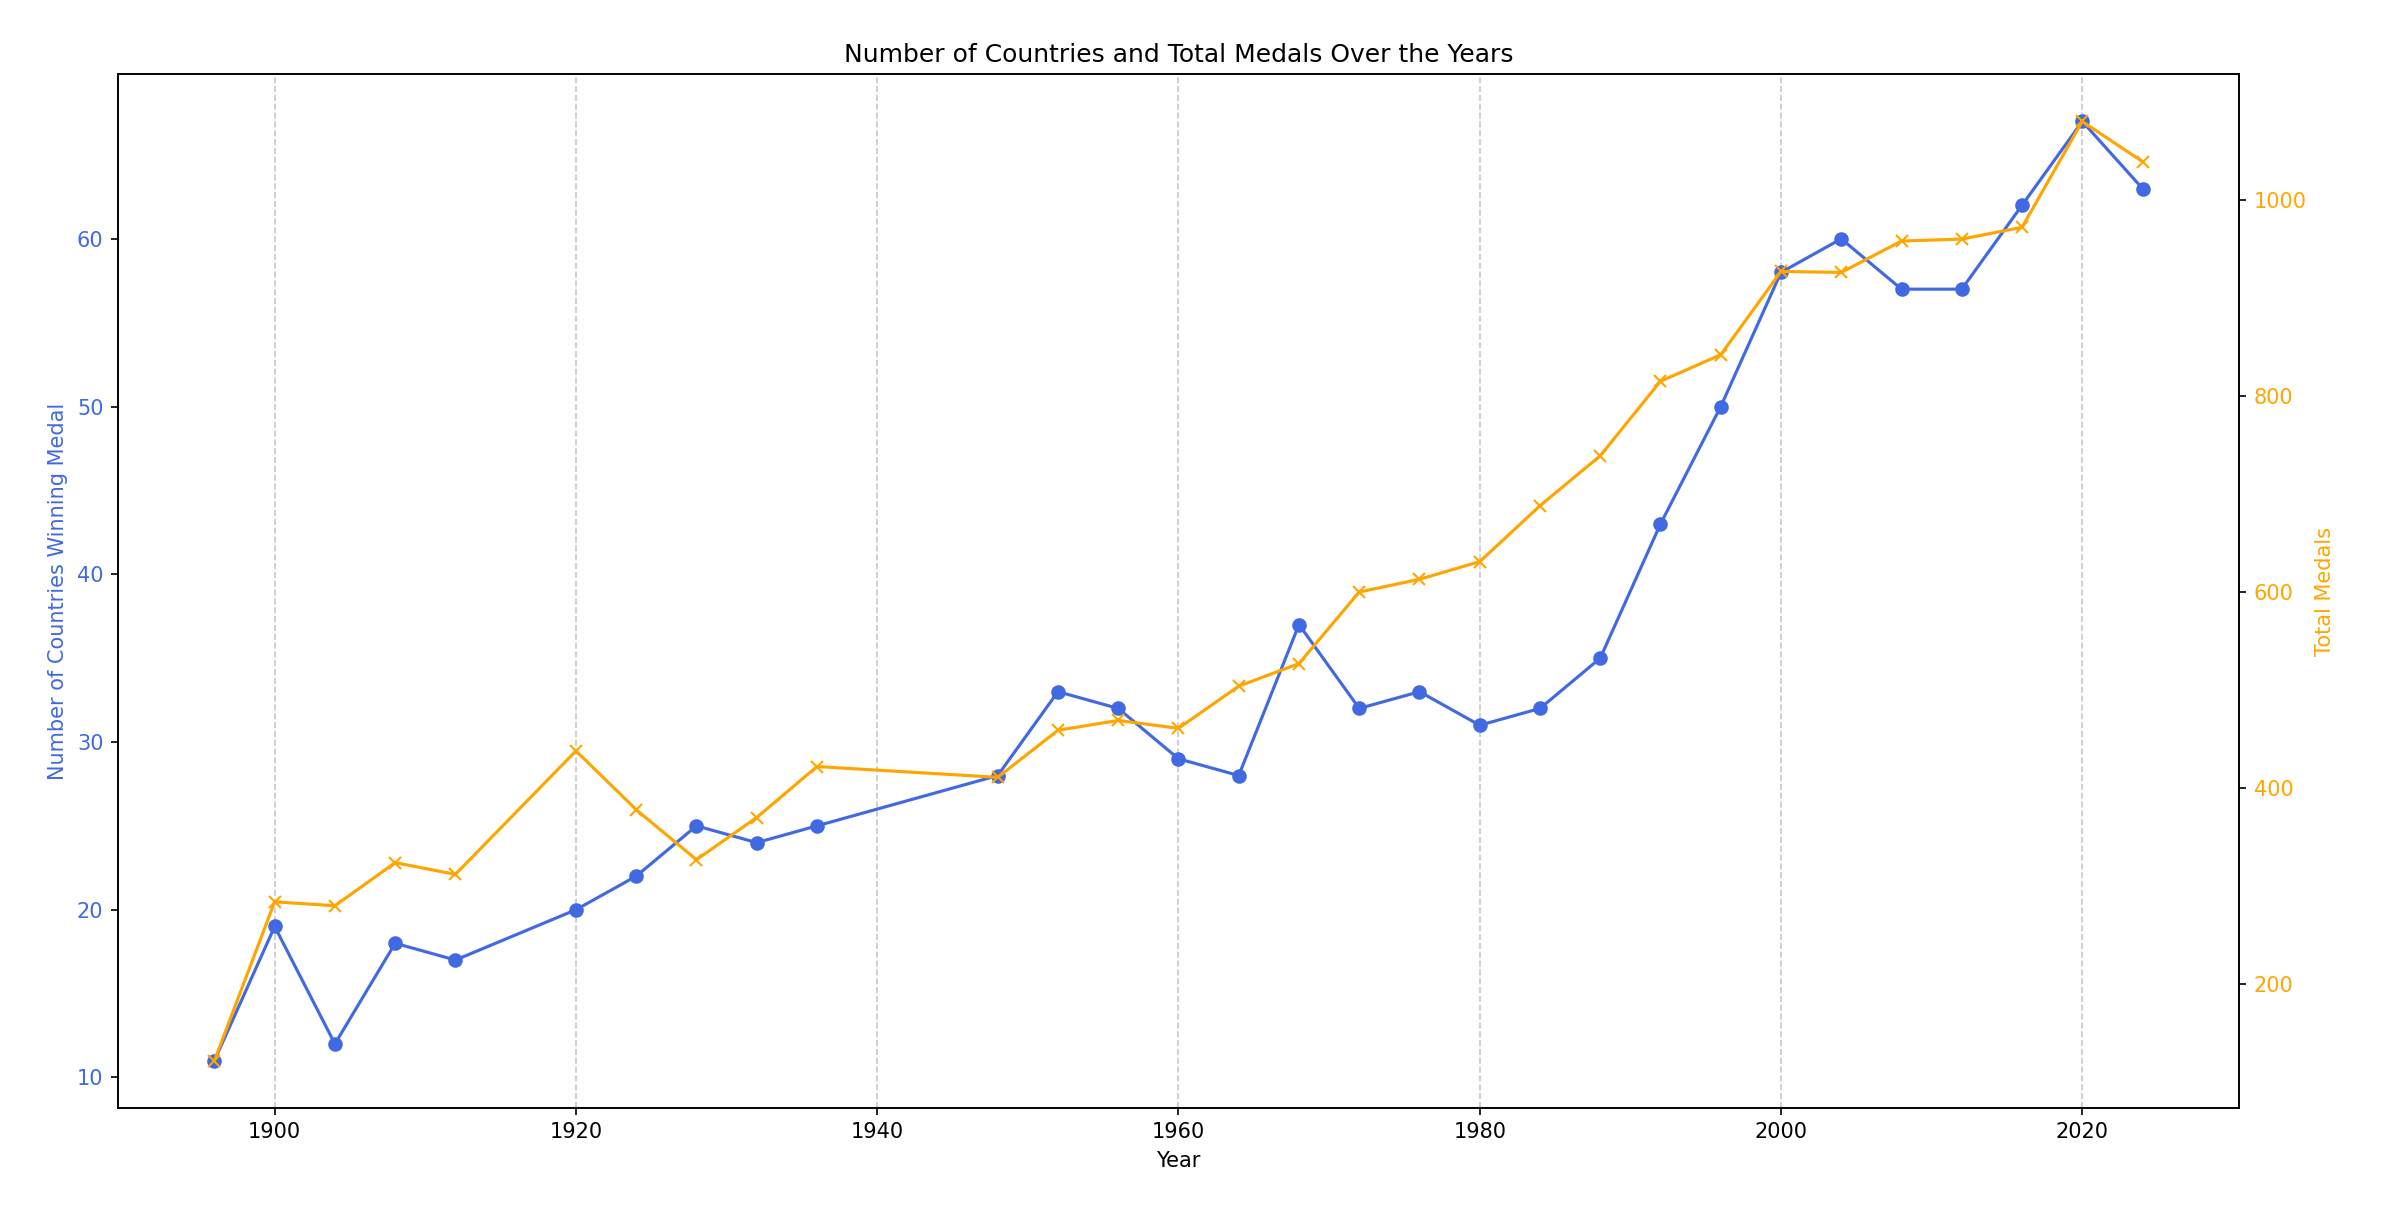
\includegraphics[width=0.5\textwidth]{MCM2025_Latex/figures/medal_total&countries_got_them.png}
    \caption{The line chart of the total number of medals and the number of medal-winning countries for each year.}
    \label{fig:medal_total&countries_got_them}
\end{figure}

We did a primary visualisation of the data, as is shown in the line chart. the overall number of the medals and countries winning the medal is growing on a general basis. This provided us some ideas of performing the data preprocessing stage. 

\section{Model Basis}

After reviewing the data, we decided to construct an \textbf{integrated macro-micro model with a focus on the micro perspective}.

Prior to developing this model, we attempted to predict national medal counts directly using time-series models, only to find the results unreliable (see \hyperref[sec:4.3]{Section 4.3} for details). We concluded that relying solely on macro-level time-series models does not explicitly represent the latent variables for analysis, which led us to shift our focus to the micro-level athlete perspective. However, using this micro-level approach, athletes who have only competed once in recent Olympics are difficult to fit due to insufficient data, and predicting the performance of potential newcomers is particularly challenging. In such cases, we must return to the macro-level national perspective.

We therefore decided to divide athletes into two categories: \textbf{veterans} (those who have competed before) and \textbf{recruits} (potential newcomers). The performance of veterans is predicted mainly on the basis of their individual past performance while receiving a little revision from the the country's strengths, while the number and performance of recruits is predicted solely on the basis of the country's past performance. The detailed process of model construction is as follows.

\subsection{The Athlete Gamma Model}

We fit each athlete into a Gamma model~\cite{2} for \textbf{each event} $\Gamma(P_{\text{max}}, a_{\text{max}}, \alpha, \beta)$:
\[
\Gamma(age) = P_{\text{max}} \cdot \left( \frac{age}{a_{\text{max}}} \right)^\alpha \cdot e^{-\beta(age-a_{\text{max}})}
\]
where $P_{\text{max}}$, $a_{\text{max}}$, $\alpha$ and $\beta$ are the particular parameters for each individual athlete. $P_{\text{max}}$ represents their peak strengths. $a_{\text{max}}$ implies whether an athlete is at their peak or in their dark hours when they enters the first Olympics.  $\alpha$ controls the increase rate of one's strength while $\beta$ controls the decay rate. It's worth mentioning that the Gamma model of each athlete of a certain country can reflect a country's strength in a certain sport field and have some latent trends as the time grows which can be predicted by time series analysis. We'll dive into this later in the following section.

We obtained ($age$, $\omega_{medal}$) from the dataset and utilized \textbf{Least Square Method} to fit every athlete into the model. Since the datasets for each (Athlete, Event) are extremely small, we introduced \textbf{regularization terms} to prevent overfitting, punishing model parameters (especially $\alpha$ and $\beta$) when extremely large when calculating the loss. The loss function is revised as follows:
\[
\mathcal{L} = \frac{1}{n} \sum_{i=1}^n (\Gamma(age) - \omega_{medal})^2 + \lambda_\alpha \cdot e^{\alpha} + \lambda_\beta \cdot e^{\beta} + \lambda_{P_{\text{max}}} \cdot P_{\text{max}}^2
\]

For athletes with only a single data point, we assigned them an average distribution based on the medal they earned in that only year . In practice, we get the mathematical expectation for simplicity. Also, special treatment was applied to the team event data (see \hyperref[appA]{Appendix A} for details). Fig~\ref{fig:GammaLoss} visualized the distribution of the variance, and the average loss is 0.7557, which is pretty good.


\begin{figure}[htbp]
    \centering
    \begin{minipage}{0.48\textwidth}
        \centering
        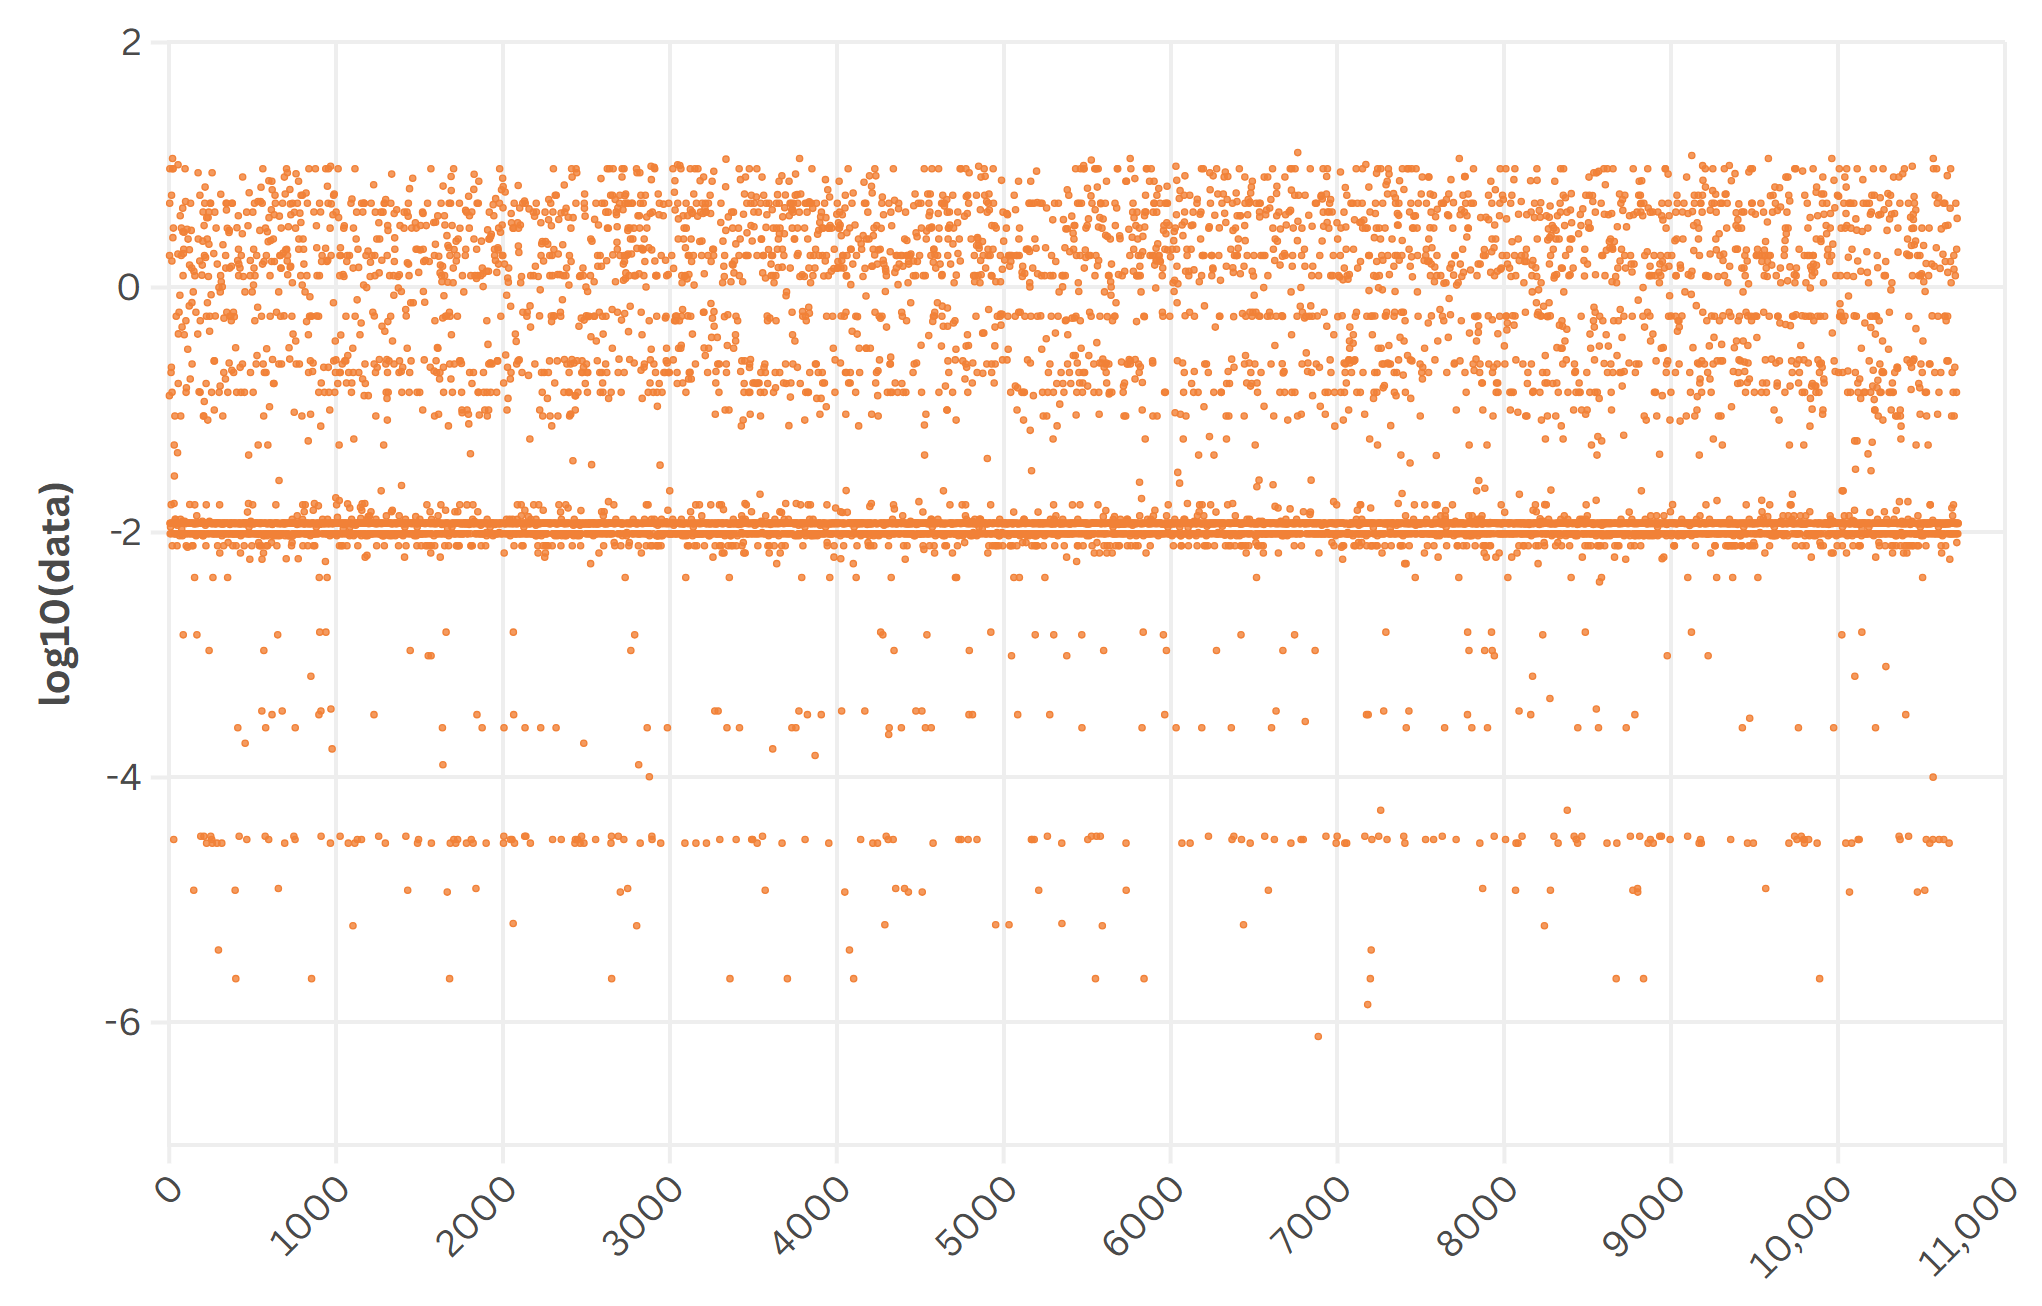
\includegraphics[width=\linewidth]{GammaLoss.png}
        \caption{Gamma Loss}
        \label{GammaLoss}
    \end{minipage}
    \hfill
    \begin{minipage}{0.48\textwidth}
        \centering
        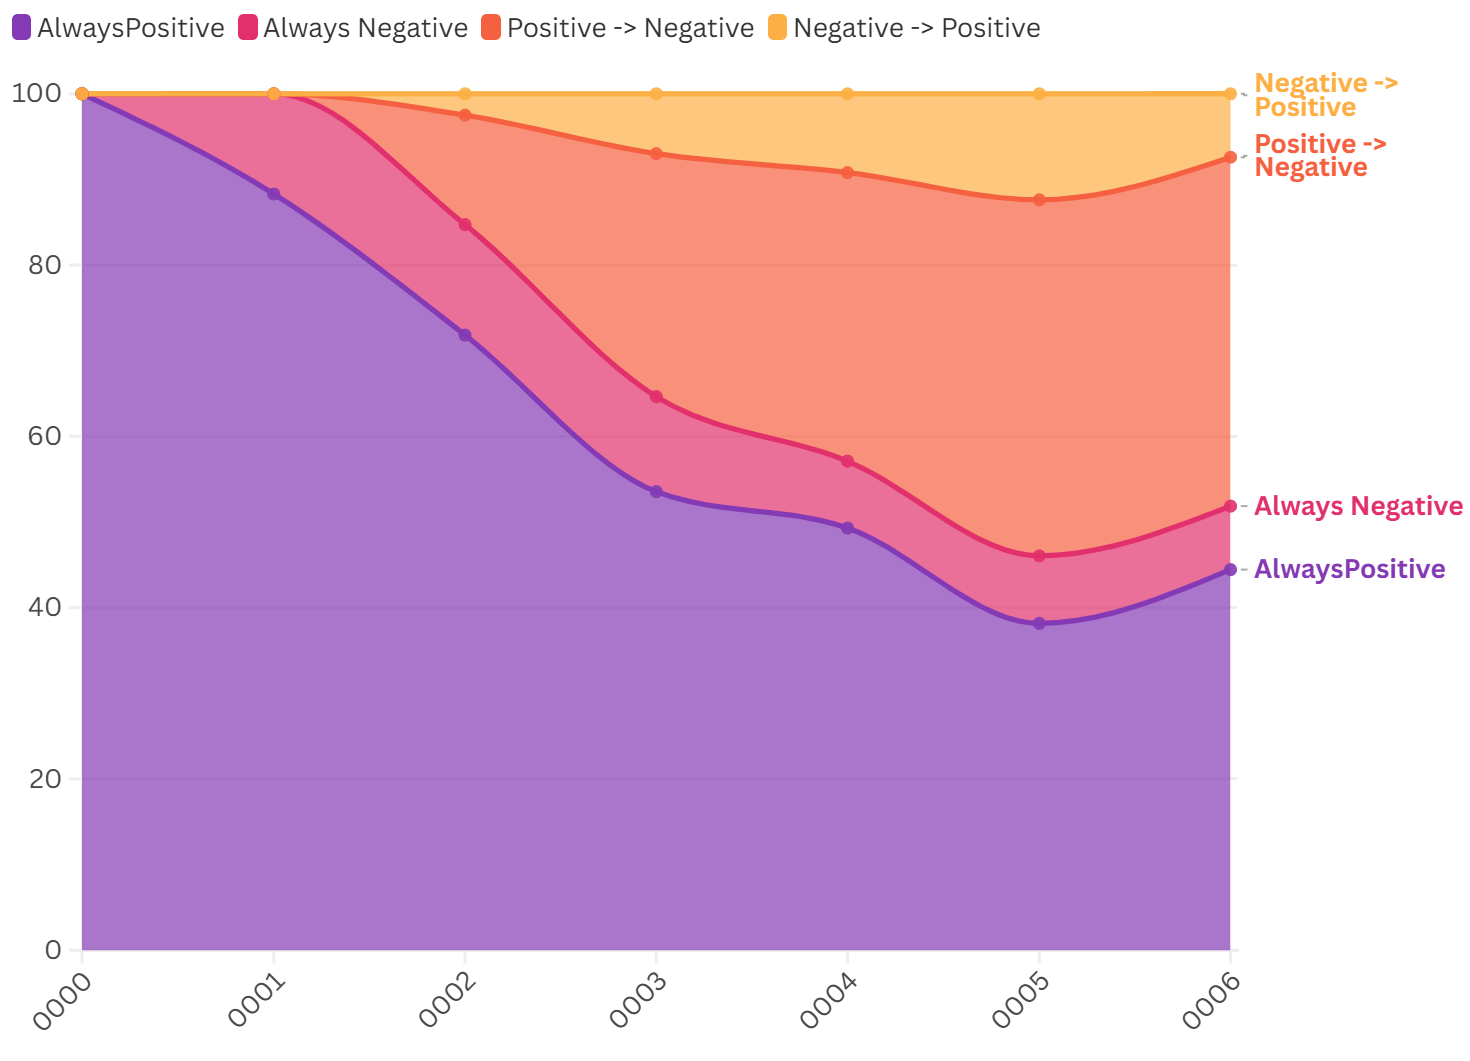
\includegraphics[width=\linewidth]{ath_change_curve.png}
        \caption{Change Curve}
        \label{ChangeCurve}
    \end{minipage}
\end{figure}

According to the data presented in Fig.~\ref{ChangeCurve}, the quantity of athletes with a performance curve that decreases first and then increases is extremely minimal, therefore it's reasonable for us to stimulate most of the athletes with Gamma function. For example, an athlete with decreasing performance has a small $a_{\text{max}}$.

\subsection{The Country / Sport Gamma Model}
\label{sec:4.2}
We define the Gamma Model of a country for a certain sport as the \textbf{distribution} of the Gamma model (a four dimensional vector$[P_{max}, a_{max}, \alpha, \beta]$) of the athlete that came out from this country. The distribution \textbf{changes over time}. To simplify our model, we arguably supposed that the distribution $P(NOC, Sport, Year) \sim \mathcal{N}(\mu,\Sigma)$, where the $\mu$ is a four-dimensional vector and the $\Sigma$ is the covariance matrix.

From this definition, we can easily conclude the fact that the close the year of the Country / Sport Gamma Model is to the current year, the more \textbf{unreliable} it is. It is because we aren't sure whether the athletes debuting in this year are actually good or bad, given that we don't know their actual performance afterwards. In \hyperref[sec:5.2]{section 5.2}, we'll solve this trouble by adopting both Time Series Analysis and Bayesian approach.

Note that time series of the Country / Sport Gamma model can be well fit into a EWMA model\cite{5}\cite{6}$$S_t = \lambda_{\text{EWMA}} \cdot X_t + (1 - \lambda_{\text{EWMA}}) \cdot S_{t-1}$$This can be validated by the fact that the probability of an acceptable prediction (average deviation of the four parameters < 0.5) is 90.2\% on the average. (We predicted 2008, 2012, 2016) It's worth mentioning that when predicting data for a certain year, we masked the data of that year and those after. The reason behind the outliers will be explored in later sections.

\section{Core Medal Prediction Modal}
To predict next year's medal counts, we built extra models and made detailed analysis on the basis of our model. 
In general, the prediction of a country is a four-dimensional vector, containing 
$\mathbb{E}[\text{'Gold'}]$ , $\mathbb{E}[\text{'Silver'}]$ , $\mathbb{E}[\text{'Bronze'}]$ and $\mathbb{E}[\text{'No Medal'}]$.
\begin{align*}
    \text{Prediction} &= \mathbb{E}[\text{Veterans}] + \mathbb{E}[\text{Recruits}] \\
    &= \sum_{i=1}^{n} x_i(p_i \cdot \text{Medal}) + \text{Medal}_c \cdot \mathbb{E}[\Delta n] + \epsilon_c + \sum \epsilon_i
\end{align*}

where $\mathbb{E}[\cdot]$is the mathematical expectation, $\Delta n$ is the number of new athletes of this event of this country, $\epsilon_c$ and $\epsilon_i$ are random effects term of countries and individuals respectively, $Medal_c$, $Medal$ are \textbf{four-dimensional one-hot vectors} and the former is sampled from the Country / Sport Gamma model distribution.

We spotted that $\epsilon_i$ can be easily neutralized \hyperref[sec:5.2]{(Section 5.2)} if the athletes of a country are enough, but countries with lower ranks suffered a lot from this uncertainty. As a result, in order to also predict how many will earn their first medal in the 2028 Olympics, we get a \textbf{two-layer} prediction model. In the first layer, we predicted for elite countries where we treat each country separately. In the second layer, however, we put unexceptional countries together to predict \textbf{'sudden medals'} on a group level. Fig~\ref{fig:Prediction Model} presents our prediction model.

\begin{figure}
    \centering
    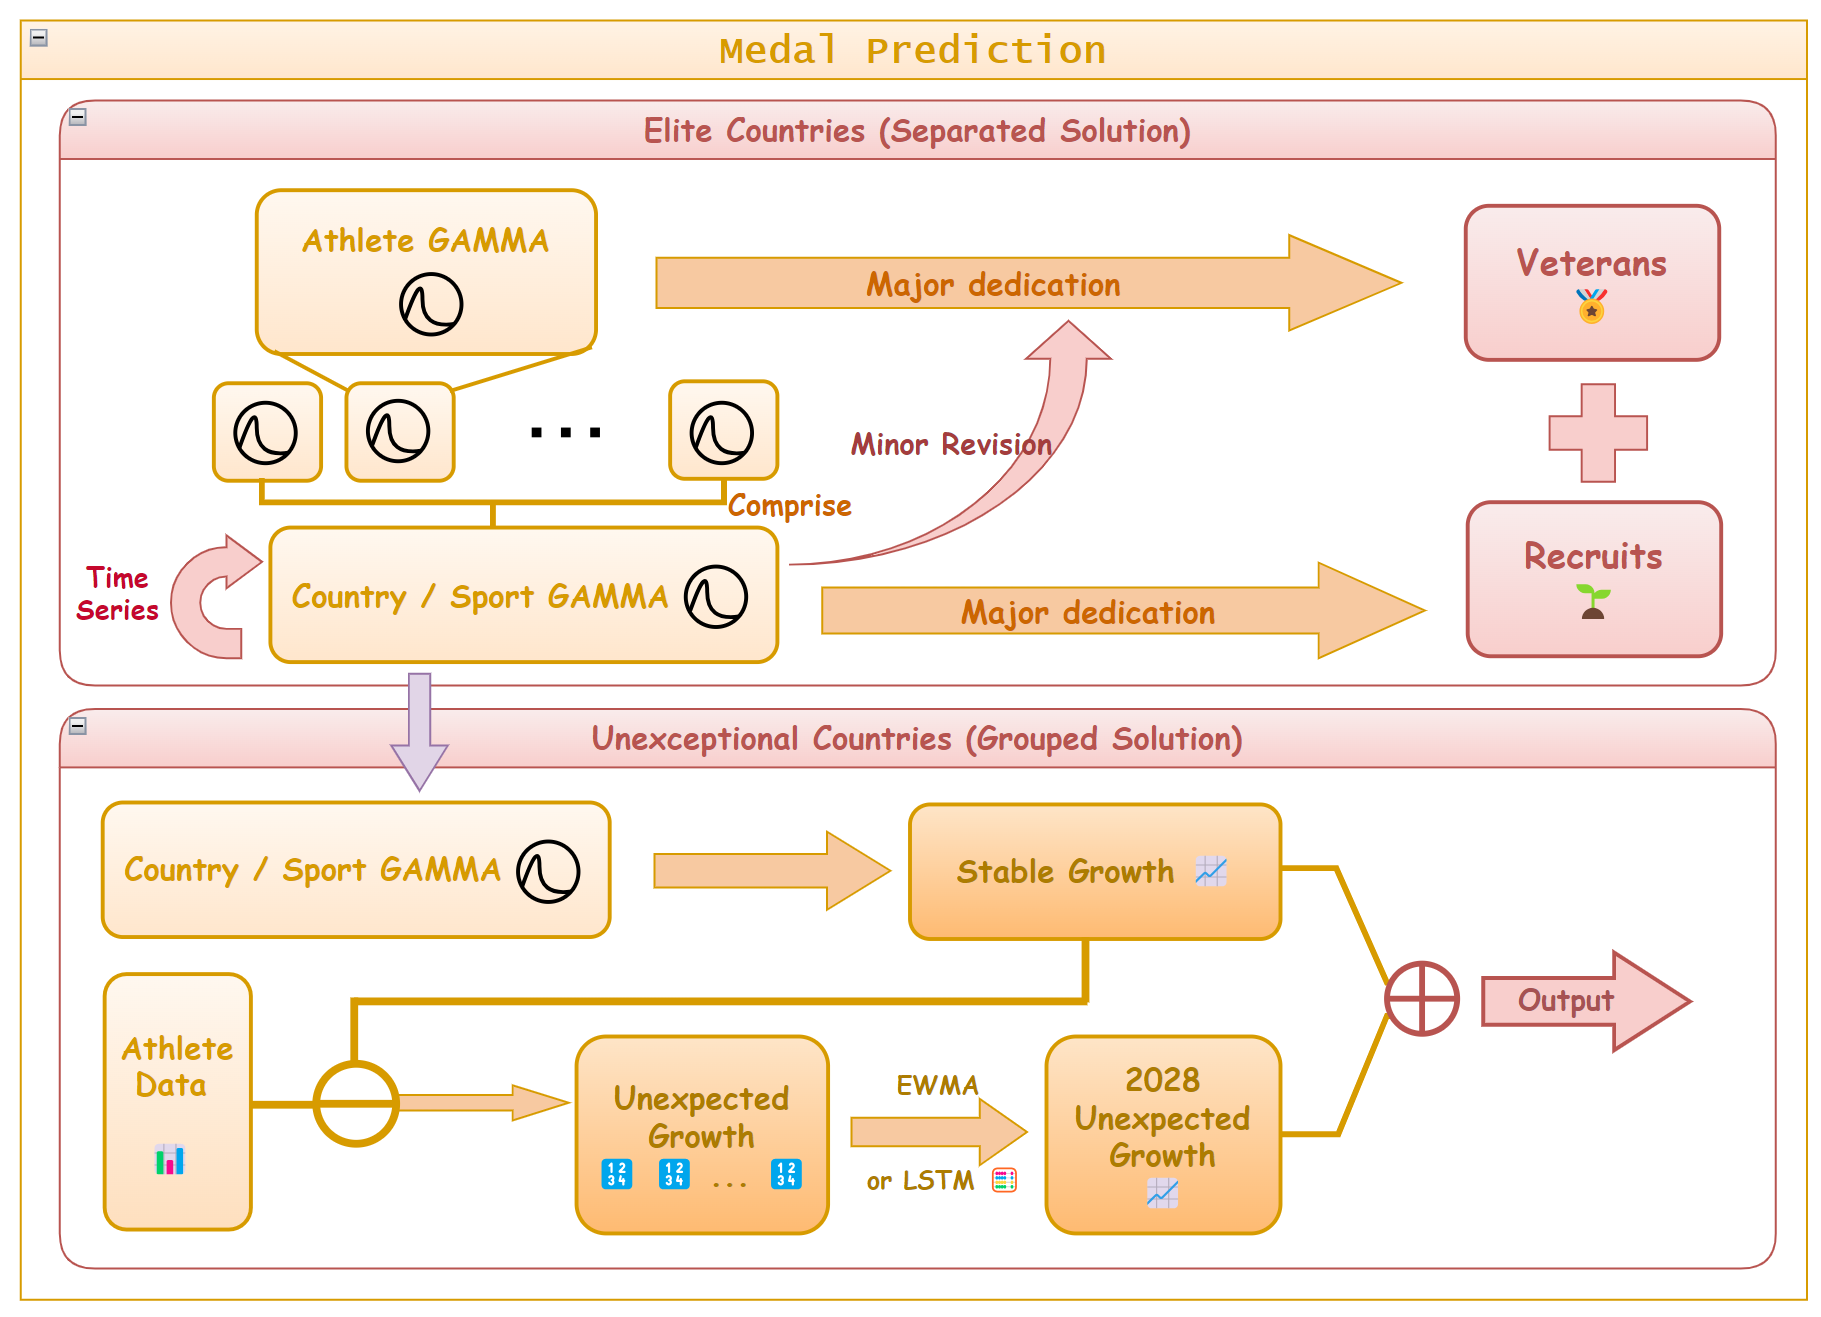
\includegraphics[width=0.7\linewidth]{Prediction Model.png}
    \caption{Prediction Model}
    \label{fig:Prediction Model}
\end{figure}

The first three subsections will dive into the first layer, while the final one will address the second layer.

\subsection{EWMA Patching Unreliable Recent Data and Predicting Recruits}
\label{sec:5.1}

In \hyperref[sec:4.2]{Section 4.2}, we mentioned the 'unreliable' problem. However, the Country / Sport Gamma models of recent year, especially 2024, are significantly important for predicting the quality of the recruits. As a result, we utilized \textbf{EWMA} to conduct time series analysis to \textbf{patch} the recent Country / Sport Gamma models. To be specific, we introduced an exponential function:
\[
f(T) = \frac{2}{1 + e^{\lambda_{\text{patch}}(T - T_{p})}} - 1
\]
where $T_{p}$ is the year to predict, which equals 2028 in this case. This function represents the percentage that we trusted the initial model. Then, we used \textbf{EWMA} to predict the Country / Sport Gamma Model for each year sequentially over time, and then patch the model for each year using the following formula:$P_{revised} = f(T) \cdot P_{original} + (1 - f(T)) \cdot P_{predicted}$. This $\lambda_{\text{patch}}$ can be learned through Linear Regression. However, to save time, we manually set four lambdas in place of $f(T)$ for 2024, 2020, 2016 and 2012.

\begin{figure}
    \centering
    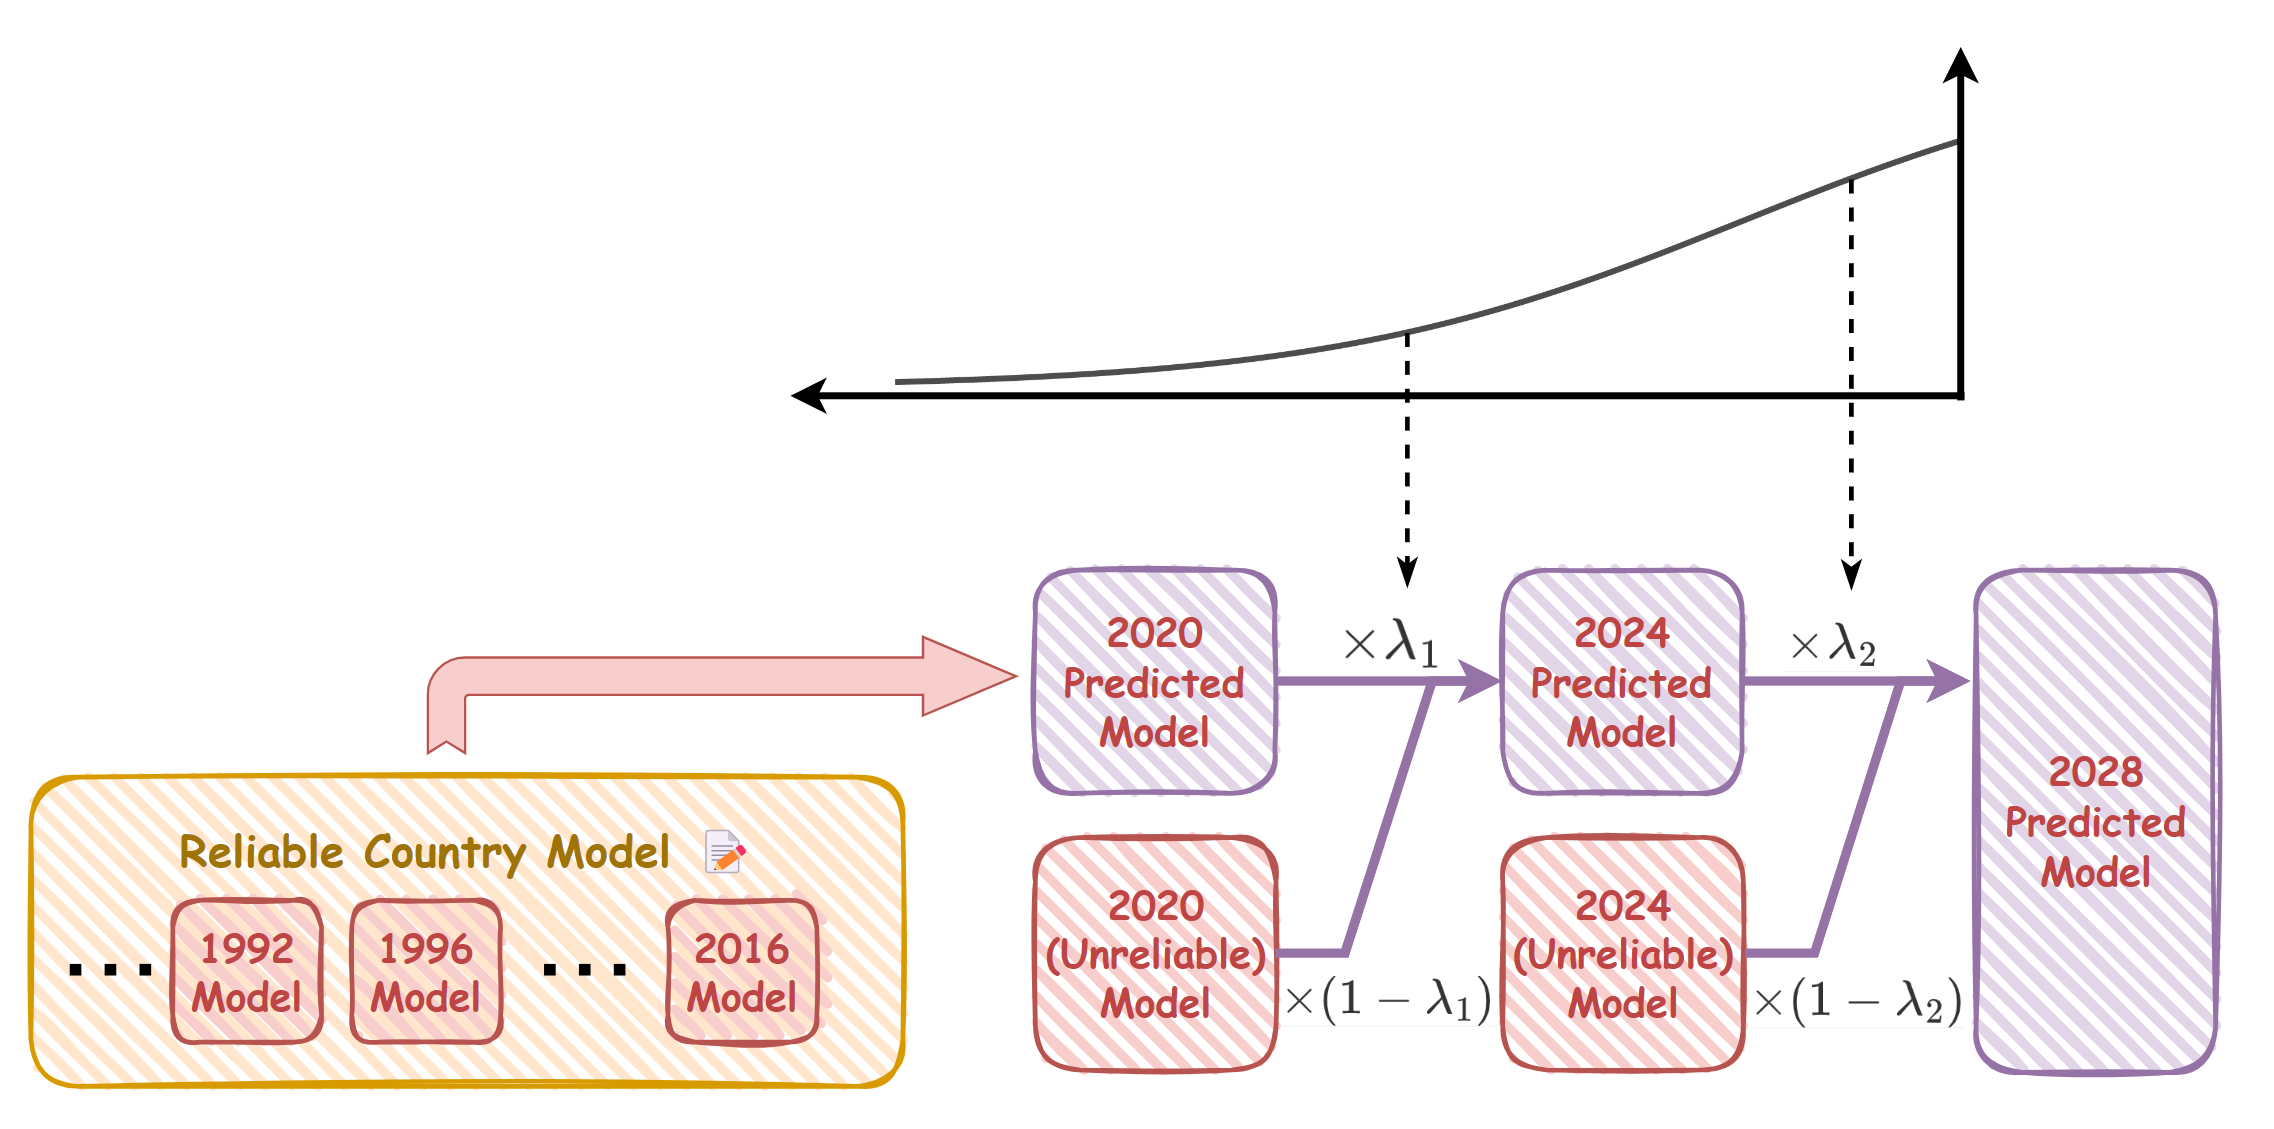
\includegraphics[width=0.6\linewidth]{The Patching Process.png}
    \caption{The Patching Process}
    \label{fig:The Patching Process}
\end{figure}

The patching process is illustrated in Fig~\ref{fig:The Patching Process}. We'll soon make further use of the patched models in the following section.
Here, we used the predicted model to get $Medal_c$. As for $\Delta n$, we introduced another EWMA model to predict. The precision of $\Delta n$ is quite accurate. (Fig~\ref{fig:Added_Number_Loss}) Take 2016 as an example. The average of the absolute value of deviation is 0.3874, and the max one is 3.83339963. Those max ones nearly all comes from the Gymnastics team of Switzerland. Fig~\ref{fig:output_gradient_blur_center} shows this result. The detail of how we deal with the data are introduced in \hyperref[appA]{Appendix A}. (Including treatment of the HC effect)
Finally, we used \textbf{Monte-Carlo Simulation} to predict the expected medal count of recruits (we predicted Gold, Silver, Bronze separately) as well as the \textbf{Prediction Interval (PI)}. For details, please refer to \hyperref[appA]{Appendix A}.

\begin{figure}[htbp]
    \centering
    \hspace*{0.1\textwidth} % 左侧添加空白
    \begin{minipage}{0.35\textwidth} % 调整宽度
        \centering
        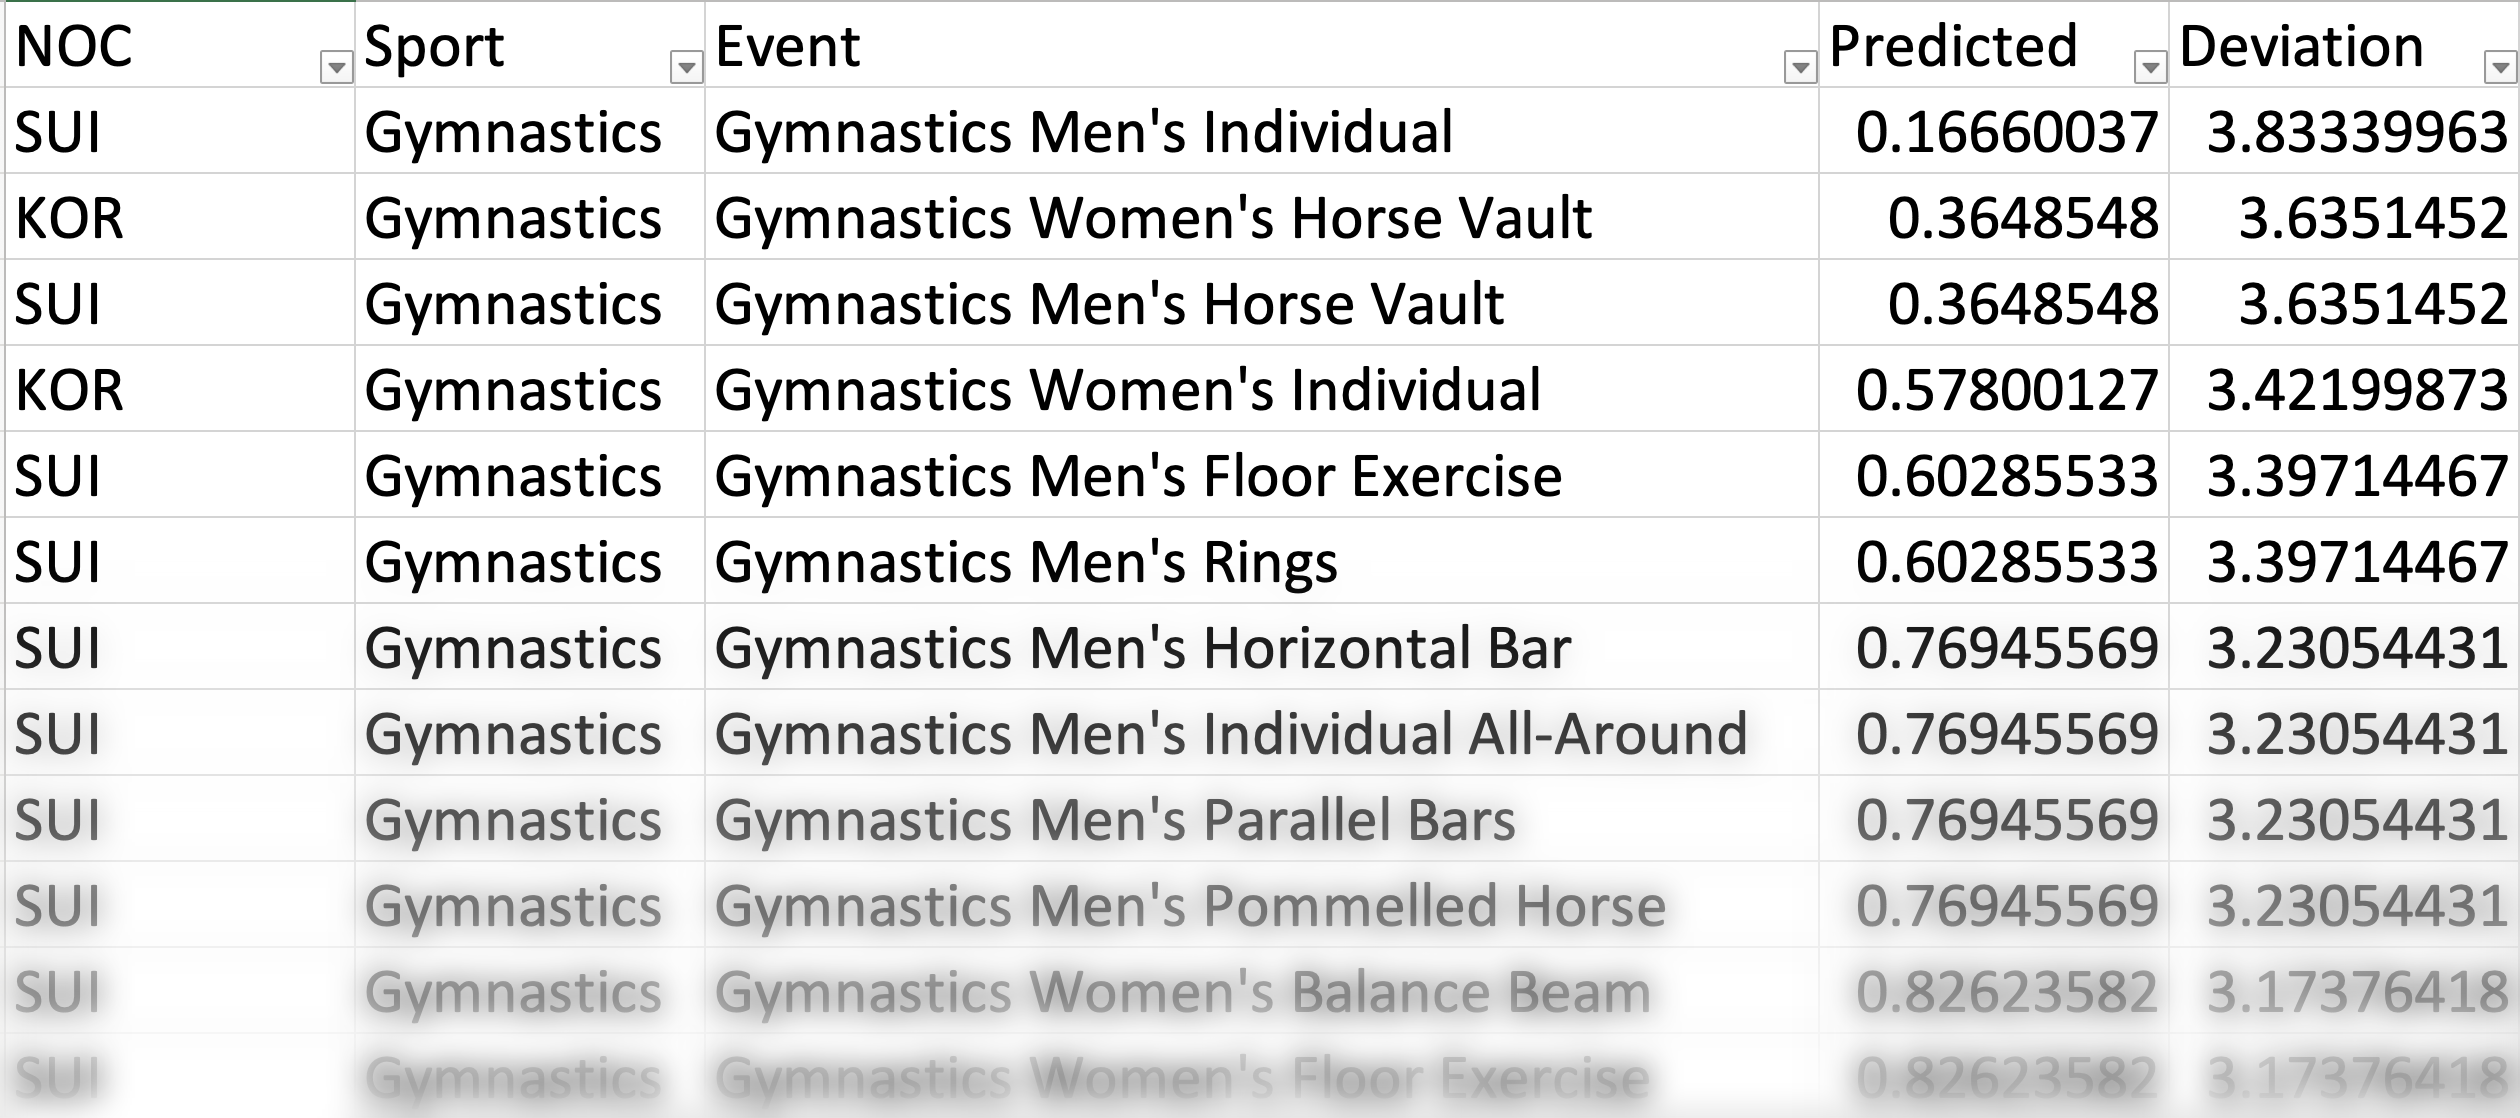
\includegraphics[width=\linewidth]{output_gradient_blur_center.png}
        \caption{Enter Caption}
        \label{fig:output_gradient_blur_center}
    \end{minipage}
    \hfill
    \begin{minipage}{0.35\textwidth} % 调整宽度
        \centering
        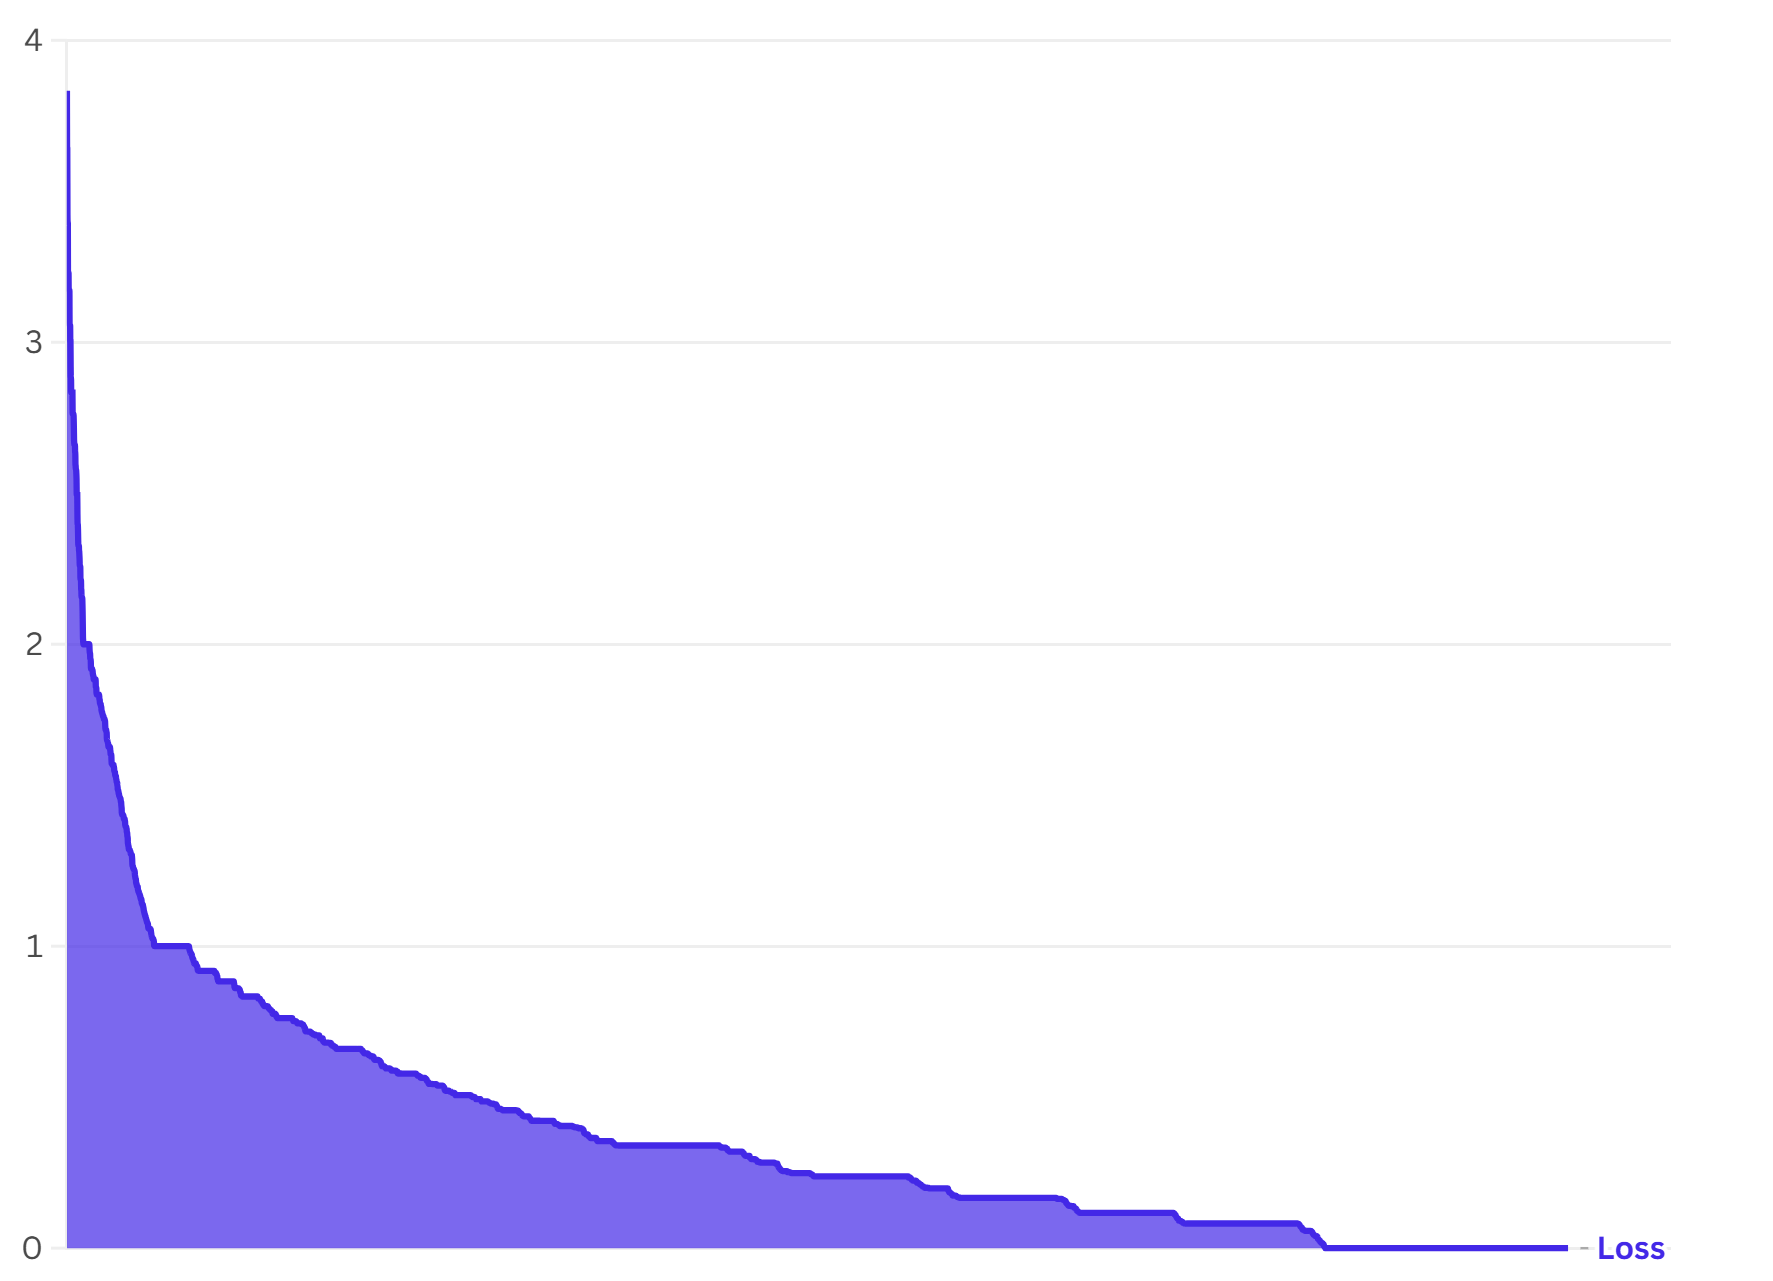
\includegraphics[width=\linewidth]{Added_Number_Loss.jpg}
        \caption{Added Number Loss}
        \label{fig:Added_Number_Loss}
    \end{minipage}
    \hspace*{0.1\textwidth} % 右侧添加空白
\end{figure}

\subsection{Bayesian For Veteran Medal Prediction}
\label{sec:5.2}

As for the task of predicting the medal of a veteran will win next year, we adopted a \textbf{Bayesian approach} to derive our predictions from both the past performance of a country and the athletes themselves. The logic of our approach is that the veterans each have a distribution of Gamma model (In the Veteran task, we simplify it as mathematical expectation as mentioned above), which is comprised of \textbf{prior probabilities}. We want to revise those probabilities by some known information, getting the \textbf{posterior probabilities}, which are more reliable. We let $s$ denote the Gamma model of a certain athlete should be, $pre$ indicate the predicted model derived from his or her past scores and $c$ is the Country / Sport Gamma model at this time. Since $p(c)$ is a macroscopic distribution, averaging over many athletes and being patched by previous data, we can arguably assume two things: $pre$ and $c$ are conditionally independent given $s$, $pre$ and $c$ are independent in the absence of conditions. So, we can safely get the following equation: (The concrete derivation is unfolded in \hyperref[appB]{Appendix B}.)
\[
p(s \mid pre, c) = \frac{p(s \mid c) \cdot p(s \mid pre)}{p(s)}.
\]

As a result, in order to get $p(s \mid pre, c)$, we only cared about $p(s \mid c)$, $p(s|pre)$ and $p(s)$. $p(s \mid c)$ equals to $p(c)$ according to our assumption, $p(s|pre)$ can be easily fit using past data, and $p(s)$ can be interpreted as the average performance of an Olympics player which can be directly derived from the whole datasets.
It's also worth mentioning that this process is actually another patching process, and if the athletes come from an early age and already have a great $p(s \mid pre)$, we needn't revise it much. So we introduced a $\lambda_{\text{rev}}$ which is determined by his or her $age$, and also follows a pattern similar to \hyperref[sec:5.1]{Section 5.1}: $P_{revised} = \lambda_{\text{rev}} P_{original} + (1 - \lambda_{\text{rev}}) P_{predicted}$

After the model was built, we validated its effectiveness. We selected the most suitable medal data from 2012 and 2016 to test the model, and used the differences to assess the model's accuracy. The total sum of all differences was calculated to be -4.510305625746792. The probability that the predicted medals exactly matched the actual results was 71.37\%.

It's worth noting that during the model development process, we found that the HC effect mainly manifests as an increase in the number of athletes from that country and a rise in the number of dominant events. However, each individual's performance changes little. Therefore, the Country / Sport Gamma Model is barely affected by this effect.

\subsection{Veterans Quitting Possibilities \& Preliminary Prediction}

Since we build a model for each athlete, it's particularly important whether a person will participate in the next competition. So, we define a probabilistic model $p$ referring to the possibility that \textit{a person} will attend next competition.
\[
p(m_{\text{last}}, t) = \sigma \left( \alpha \cdot \omega_{m_{\text{last}}}) - \beta e^{t} \right)
\]
where $\sigma(\cdot)$ denotes the Log-Likelihood Function used in \textbf{Logistic Regression}, $m_{\text{last}}$, $t$ refer to the medal the person won in the previous year and the times he or she has attended the event respectively. $\alpha$ and $\beta$ are the parameters that need to be learned.

We used \textbf{Gradient Descent} to solve it and the average training score is $Score_t = 0.8369 > 0.8$, which demonstrated a satisfactory training performance (the distribution of $Score_t$ is shown in Fig~\ref{fig:p-value_distribution}).

\begin{figure}[htbp]
    \centering
    \hspace*{0.1\textwidth} % 左侧添加空白
    \begin{minipage}{0.35\textwidth} % 调整宽度
        \centering
        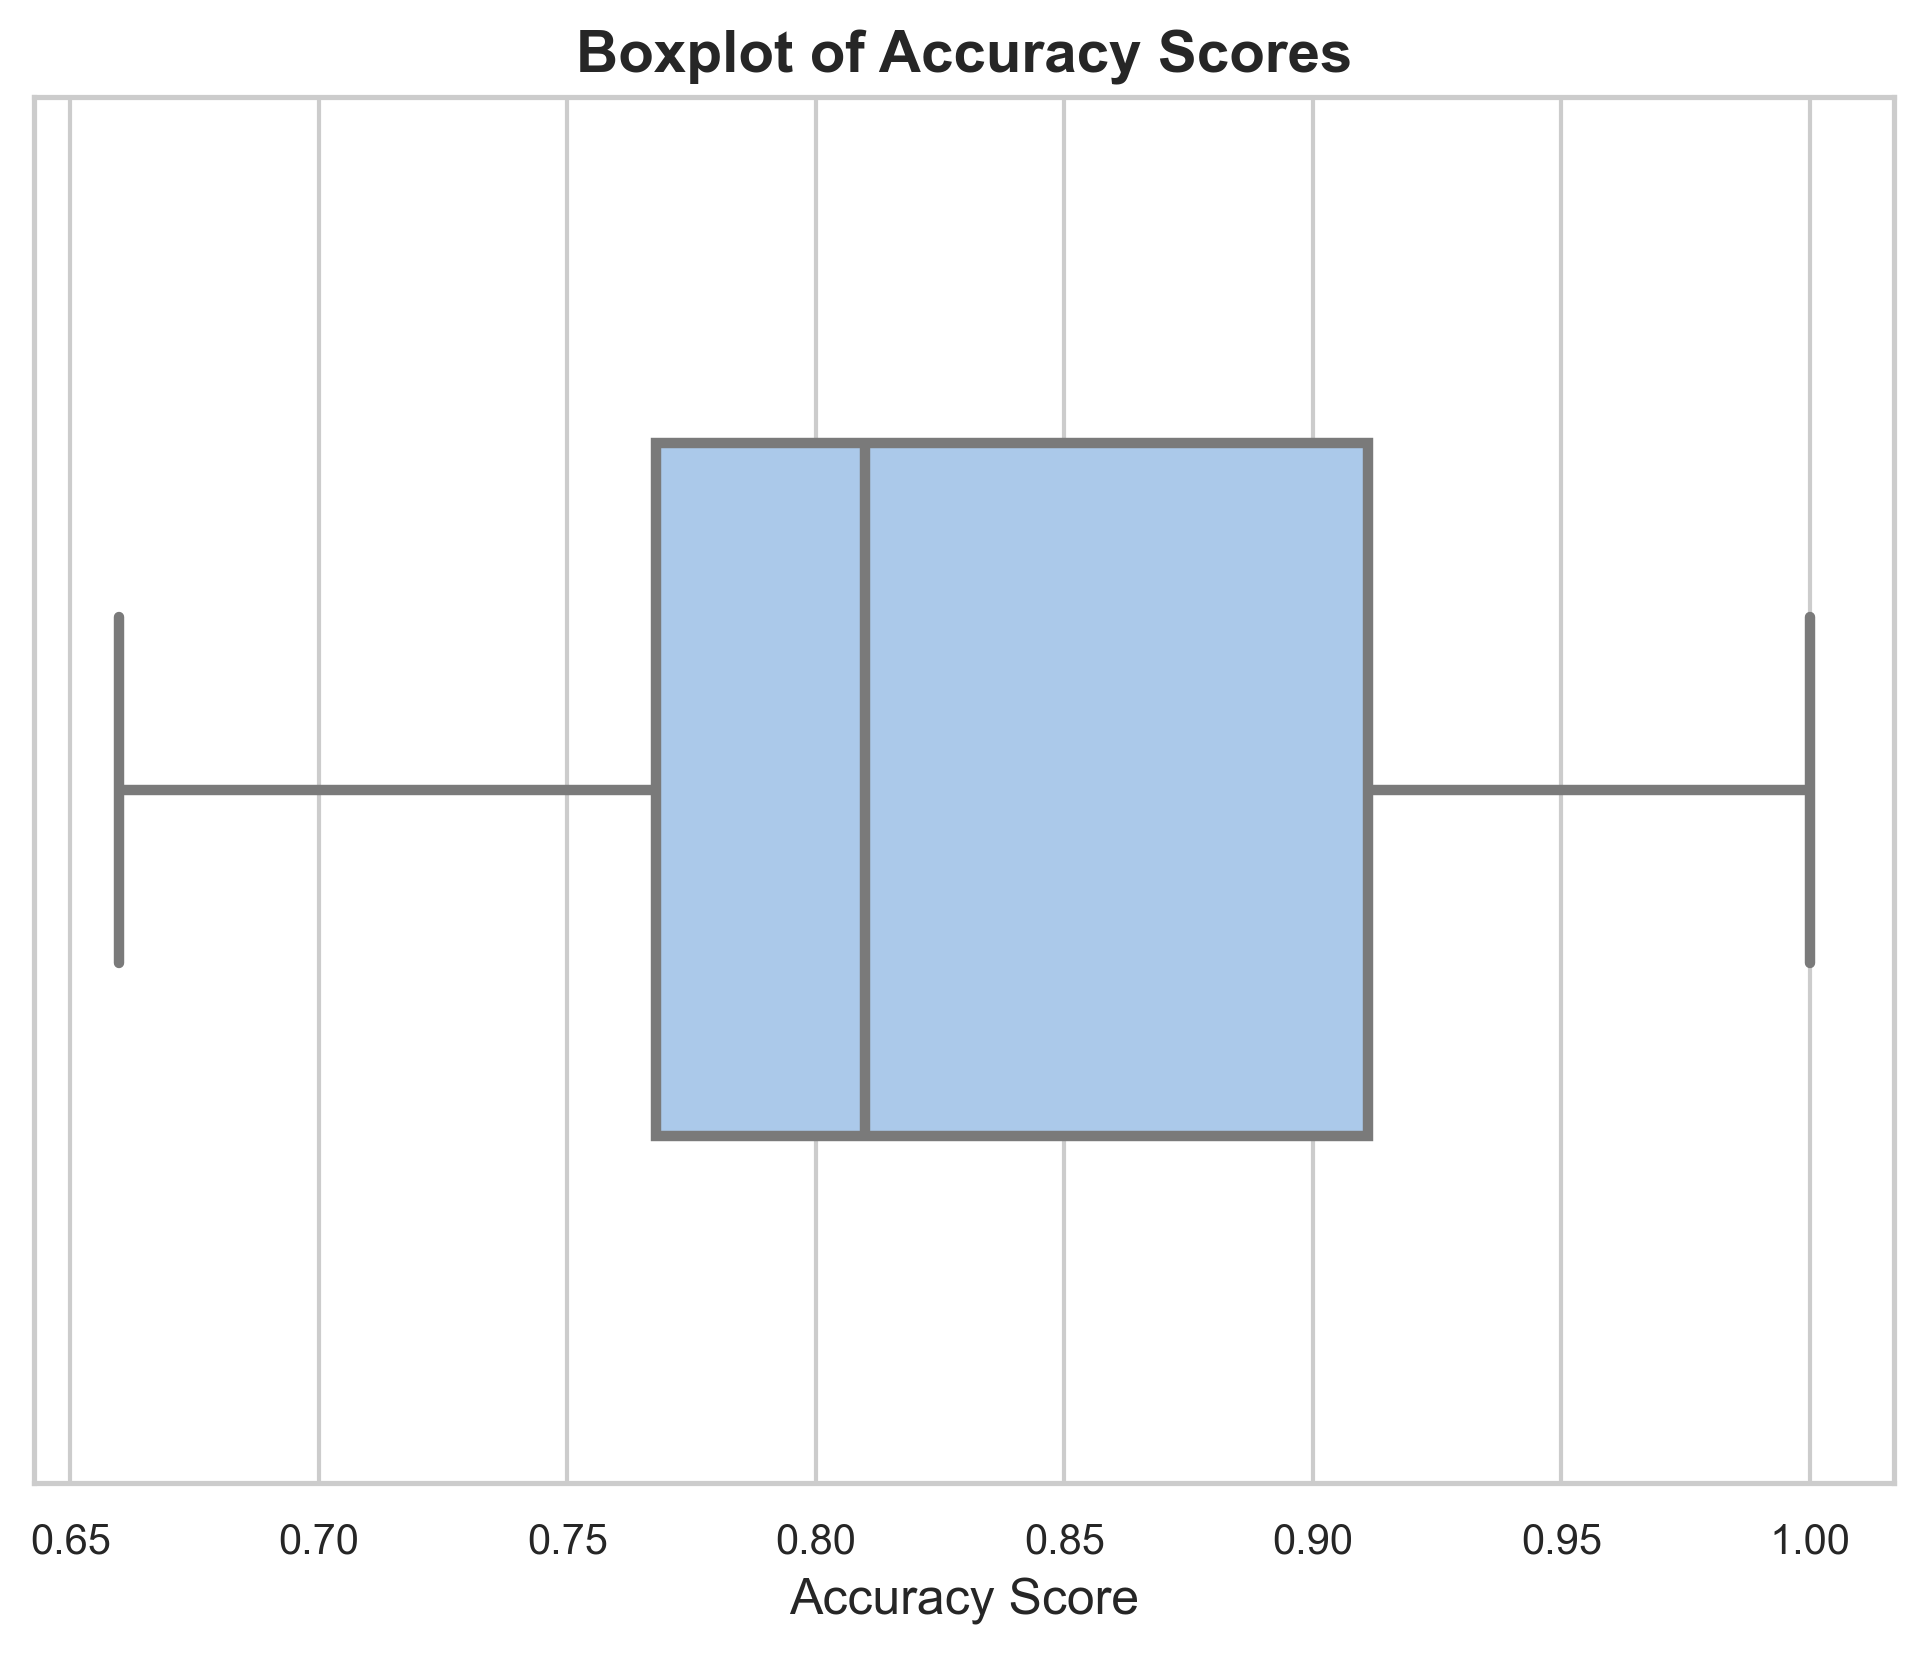
\includegraphics[width=\linewidth]{boxplot_accuracy_scores_1.png}
        \caption{Distribution $Score_t$ obtained through training.}
        \label{fig:p-value_distribution}
    \end{minipage}
    \hfill
    \begin{minipage}{0.4\textwidth} % 调整宽度
        \centering
        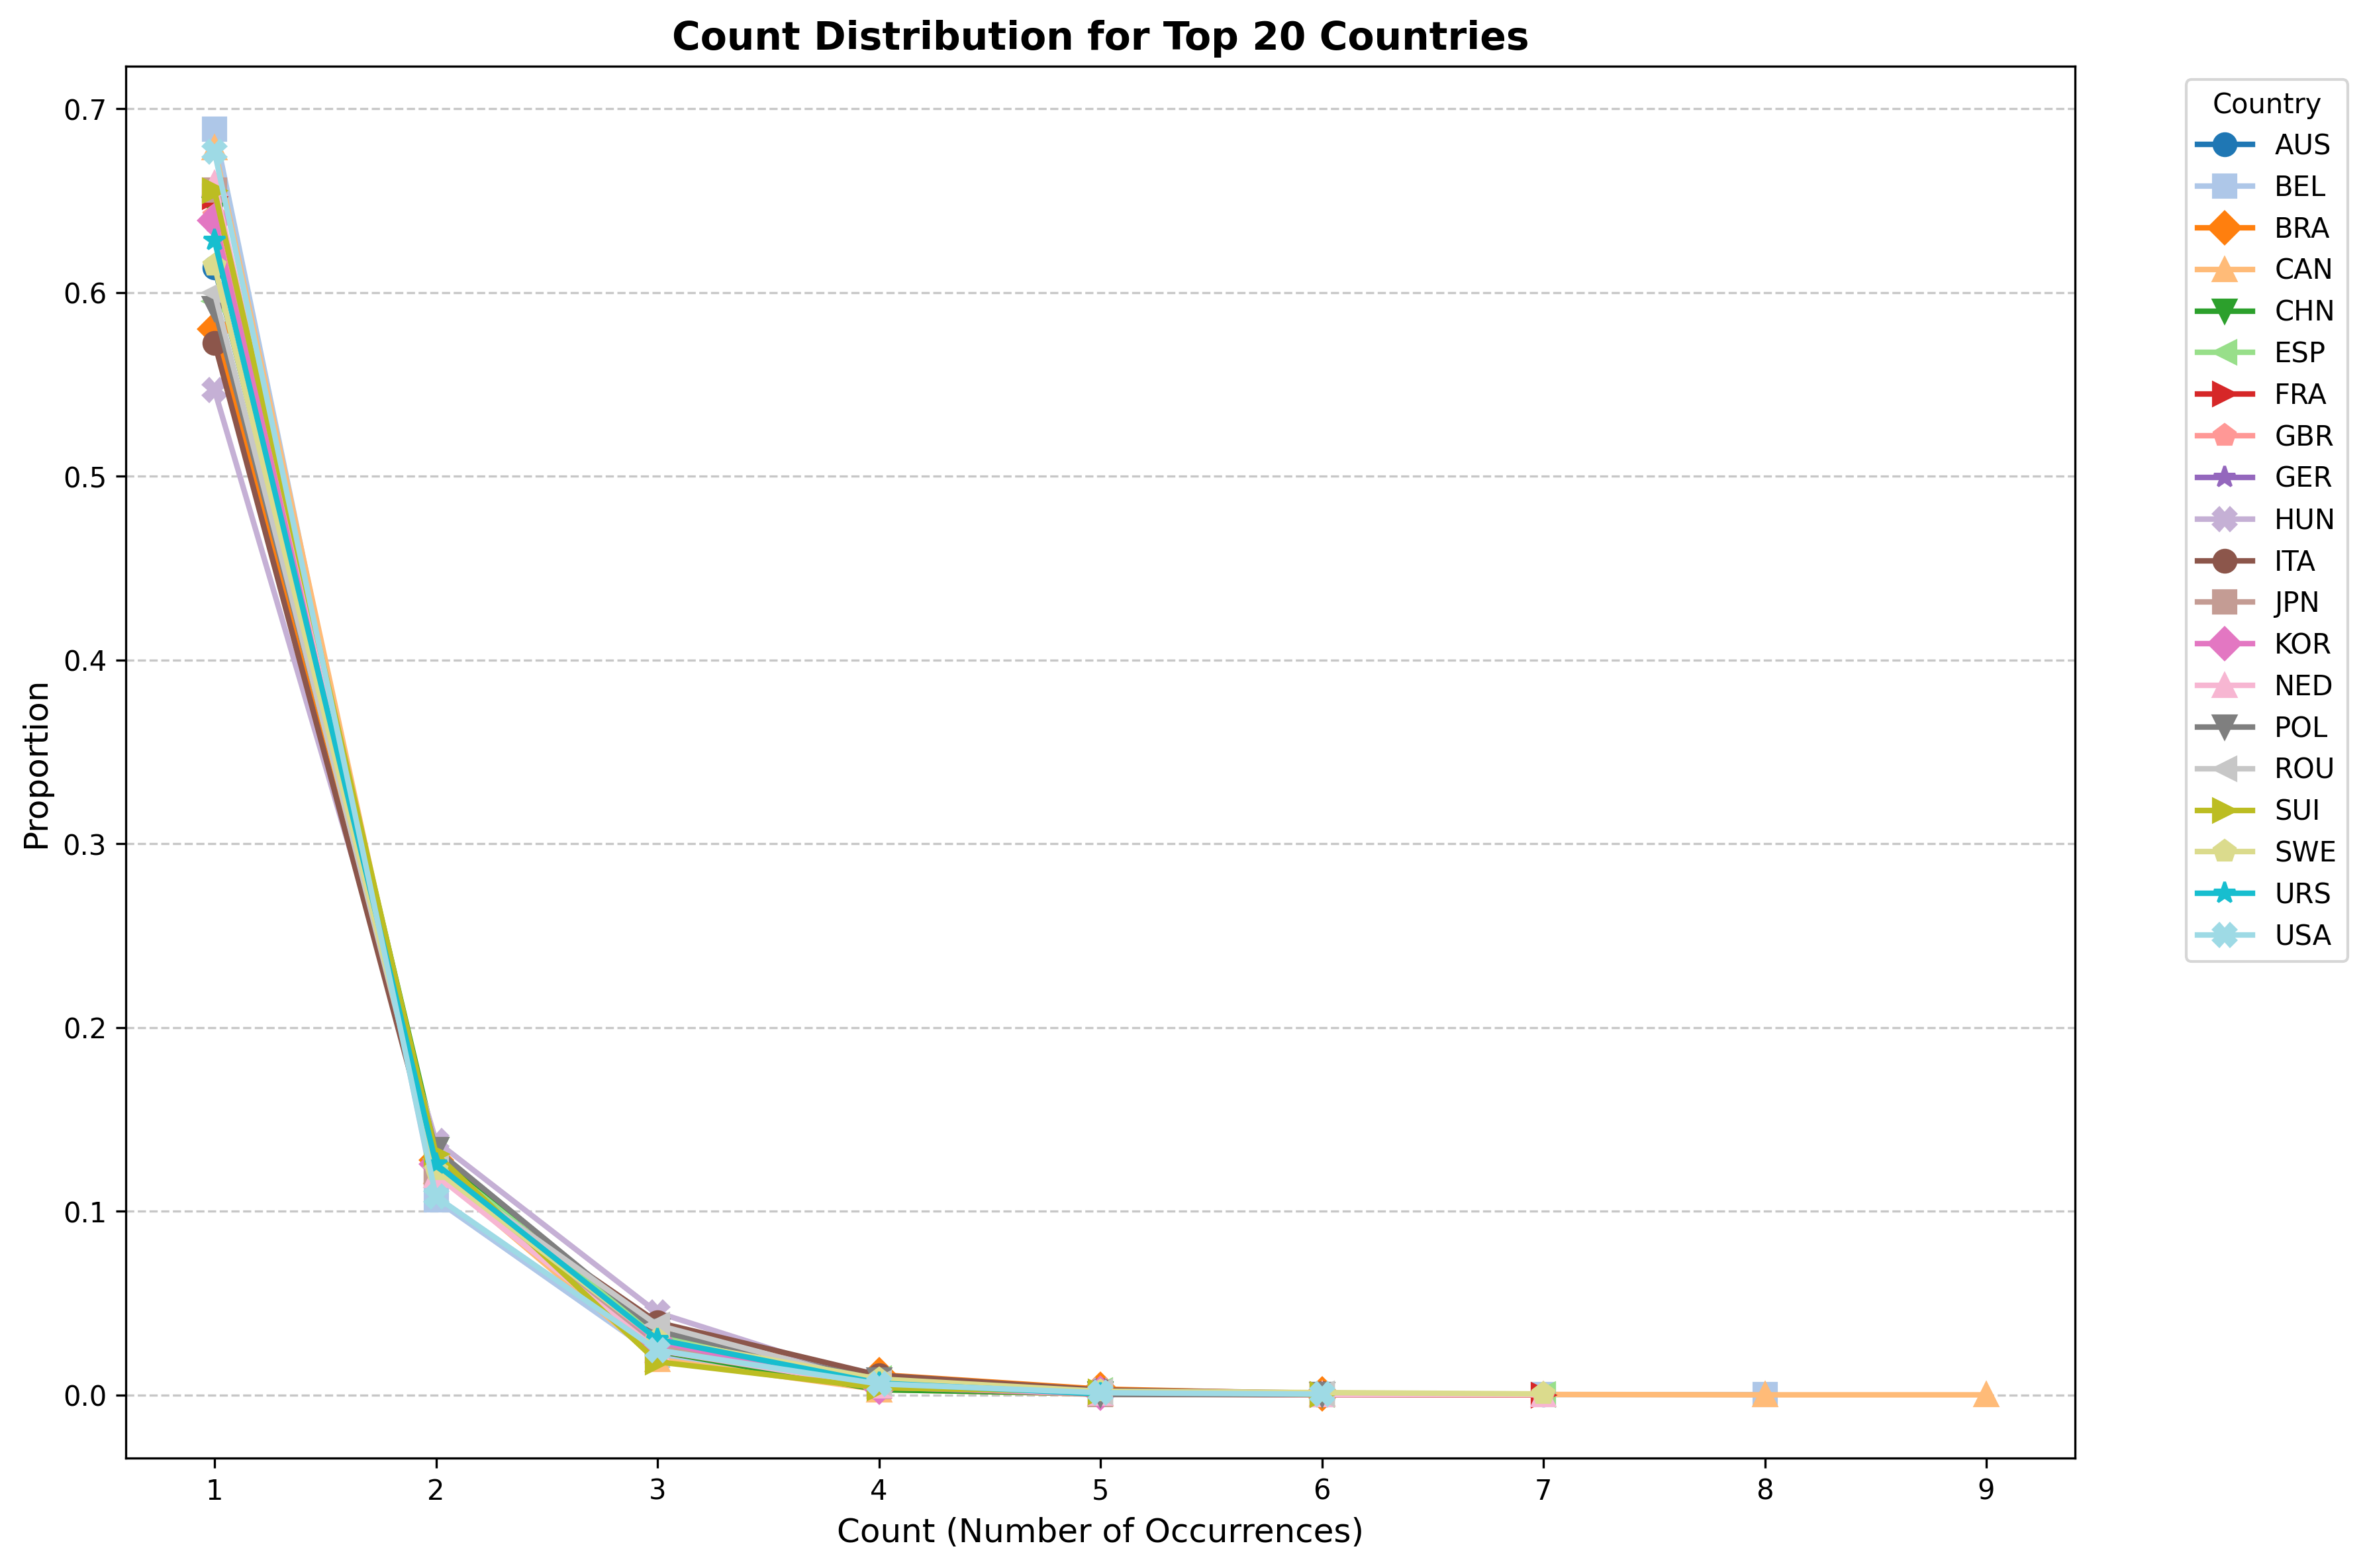
\includegraphics[width=\linewidth]{MCM2025_Latex/figures/count_distribution_top_20_countries.png}
        \caption{Count distribution of the top 20 countries.}
        \label{fig:count_distribution_top_20_countries}
    \end{minipage}
    \hspace*{0.1\textwidth} % 右侧添加空白
\end{figure}


For further verification of this model, we've proved that the probability is not concerned with \textit{the country} of the athletes by adopting the \textbf{Kruskal-Wallis Test}. We calculated p-value: $p = 0.99675 > 0.05$ and it's acceptable.

For veterans, however, since we replaced distributions with mathematical expectations for simplicity, it's hard to get a PI for every individual. But the $p_i$ discussed in this section is a probabilistic model, offering possibilities for simulations. So we applied similar \textbf{Monte-Carlo Simulation} to get the PI for veterans when predicting 2028 medal counts.
So far, the \textbf{elite countries} part comes to an end, we directly added up the PI of veterans and the PI of recruits and get the following results. (In this section, we simply assumed that the sport of 2028 is the same as 2024, and we consider the change of the event amount in existing sports)

\begin{table}[ht]
\centering
\resizebox{0.5\textwidth}{!}{ % 缩放表格到页面的一半宽度
\begin{tabular}{|c|c|c|c|c|c|}
\hline
 & \multirow{2}{*}{\textbf{Loss}} & \multicolumn{4}{c|}{\textbf{Variance}} \\
\cline{3-6}
 & & \textbf{Gold} & \textbf{Silver} & \textbf{Bronze} & \textbf{Total} \\
\hline
\multirow{2}{*}{\textbf{Veteran}} & \textbf{2012} & 12.1834 & 7.0192 & 7.6786 & 15.0648 \\
                                  & \textbf{2016} & 9.1383 & 8.5047 & 11.5399 & 22.7080 \\
\hline
\multirow{2}{*}{\textbf{All}}     & \textbf{2012} & 134.4594 & 293.8373 & 401.1429 & 602.2451 \\
                                  & \textbf{2016} & 106.5606 & 144.4103 & 185.4984 & 361.1033 \\
\hline
\end{tabular}
}
\caption{Variance Table with Empty Top Left Cell}
\end{table}



We particularly focused on the top two countries, United States and China. To our satisfaction, the model can accurately predict a phenomenon that United States usually have similar gold, silver, bronze counts and are all very high and China have high gold counts but relatively low silver, bronze counts. Table 2 is an example, showing the real counts and predicted counts in 2016.
 

\begin{table}[htbp]
\centering
\caption{Medal Predictions and True Values}
\label{tab:medals}
\resizebox{0.5\textwidth}{!}{ % 缩放表格到页面的一半宽度
\begin{tabular}{|c|c|c|c|}
\hline
 & \textbf{Gold} & \textbf{Silver} & \textbf{Bronze} \\ \hline
\textbf{USA All True}       &46 &37 &38 \\ \hline
\textbf{USA All Predicted}            & 43.45084855 & 39.56983619 & 44.90724692 \\ \hline
\textbf{China All True}     &26	&18	&26 \\ \hline
\textbf{China All Predicted}          & 34.9829136 & 19.74928595 & 21.64751901 \\ \hline
\end{tabular}
}
\end{table}

It's worth mentioning that we didn't choose to predict 2020 due to the fact that literally \textbf{all} no athletes from the 2016 dataset participated in the 2020 Games, and we included rough consideration of new events (based on Country / Sport Gamma model) when predicting results for years before 2028.

From the form, we delightedly spotted a good prediction result of veteran performance, but when it comes to the recruits, the losses are unacceptable. Starting from \hyperref[sec:6]{Section 6}, we'll continue to patch this model to correct the accuracy.

For the 2028 medal count prediction, we listed top 10 countries' medal counts and whether a country improves or becomes worse is illustrated by \textbf{rank change} and \textbf{medals differences} in the final prediction section (i.e., \hyperref[sec:9]{Section 9}). Improve Countries: USA, GBR, JPN, KOR, IRI, ESP, PRK, JAM. Worse Countries: CHN, AUS, FRA, ITA, NED.

It's worth noting that this is just the \textbf{preliminary prediction result}, because we assumed that the events of the 2028 didn't change compared with 2024 in this model. We'll conduct more detailed analysis relevant to event change in the later section and modify this table a little.

%内链,可能不是section 9了,注意
\begin{table}[htbp]
\centering
\caption{2028 Predicted Medal Table}
\resizebox{0.5\textwidth}{!}{ % 缩放表格到页面的一半宽度
\begin{tabular}{|c|c|c|c|c|}
\hline
& \textbf{Gold} & \textbf{Silver} & \textbf{Bronze} & \textbf{Total} \\ \hline
\textbf{USA} & 49.00 $\pm$ 4.27 & 42.06 $\pm$ 3.89 & 34.59 $\pm$ 4.56 & 125.7 $\pm$ 6.12 \\ \hline
\textbf{CHN} & 39.88 $\pm$ 3.45 & 20.44 $\pm$ 2.78 & 23.90 $\pm$ 3.12 & 84.21 $\pm$ 4.56 \\ \hline
\textbf{GBR} & 19.32 $\pm$ 1.23 & 18.58 $\pm$ 1.45 & 17.31 $\pm$ 1.67 & 55.21 $\pm$ 2.12 \\ \hline
\textbf{JPN} & 18.99 $\pm$ 1.34 & 10.45 $\pm$ 1.12 & 19.57 $\pm$ 1.45 & 49.01 $\pm$ 1.98 \\ \hline
\textbf{KOR} & 14.98 $\pm$ 1.23 & 4.769 $\pm$ 1.01 & 10.56 $\pm$ 1.34 & 30.31 $\pm$ 1.56 \\ \hline
\textbf{GER} & 12.51 $\pm$ 1.12 & 14.26 $\pm$ 1.23 & 16.77 $\pm$ 1.45 & 43.54 $\pm$ 1.89 \\ \hline
\textbf{AUS} & 10.21 $\pm$ 1.01 & 6.707 $\pm$ 1.12 & 12.94 $\pm$ 1.23 & 29.86 $\pm$ 1.67 \\ \hline
\textbf{FRA} & 8.663 $\pm$ 1.12 & 14.05 $\pm$ 1.23 & 14.78 $\pm$ 1.34 & 37.49 $\pm$ 1.78 \\ \hline
\textbf{IRI} & 7.983 $\pm$ 1.01 & 0.655 $\pm$ 0.12 & 5.685 $\pm$ 0.23 & 14.32 $\pm$ 0.67 \\ \hline
\textbf{ITA} & 7.879 $\pm$ 1.12 & 7.740 $\pm$ 1.01 & 12.76 $\pm$ 1.23 & 28.38 $\pm$ 1.56 \\ \hline

\end{tabular}
}
\end{table}


\subsection{Predictions for unexceptional Countries}
In this layer, we mainly focused on predicting unprecedented medals, i.e. how many countries win their first medal in a certain sport, which will be denoted by event $A$, and if this medal is exactly the first Olympic medal for this country (not only for a certain sport), represented by event $B$. Obviously, $\mathbb{E}[B]$ is the answer for "how many will earn their first medal in the next Olympics" (which we denote as $res$ later).

We counts the occurrence of event $A$ and event $B$ respectively and the results are visualized below. They already seem to have a strong relation but we need more detailed analysis. (It's worth noting that the outlier 2020 is the consequence of COVID-19: lots of events are changed.)

\begin{figure}[htbp]
    \centering
    \hspace*{0.1\textwidth} % 左侧添加空白
    \begin{subfigure}[b]{0.35\textwidth} % 调整宽度
        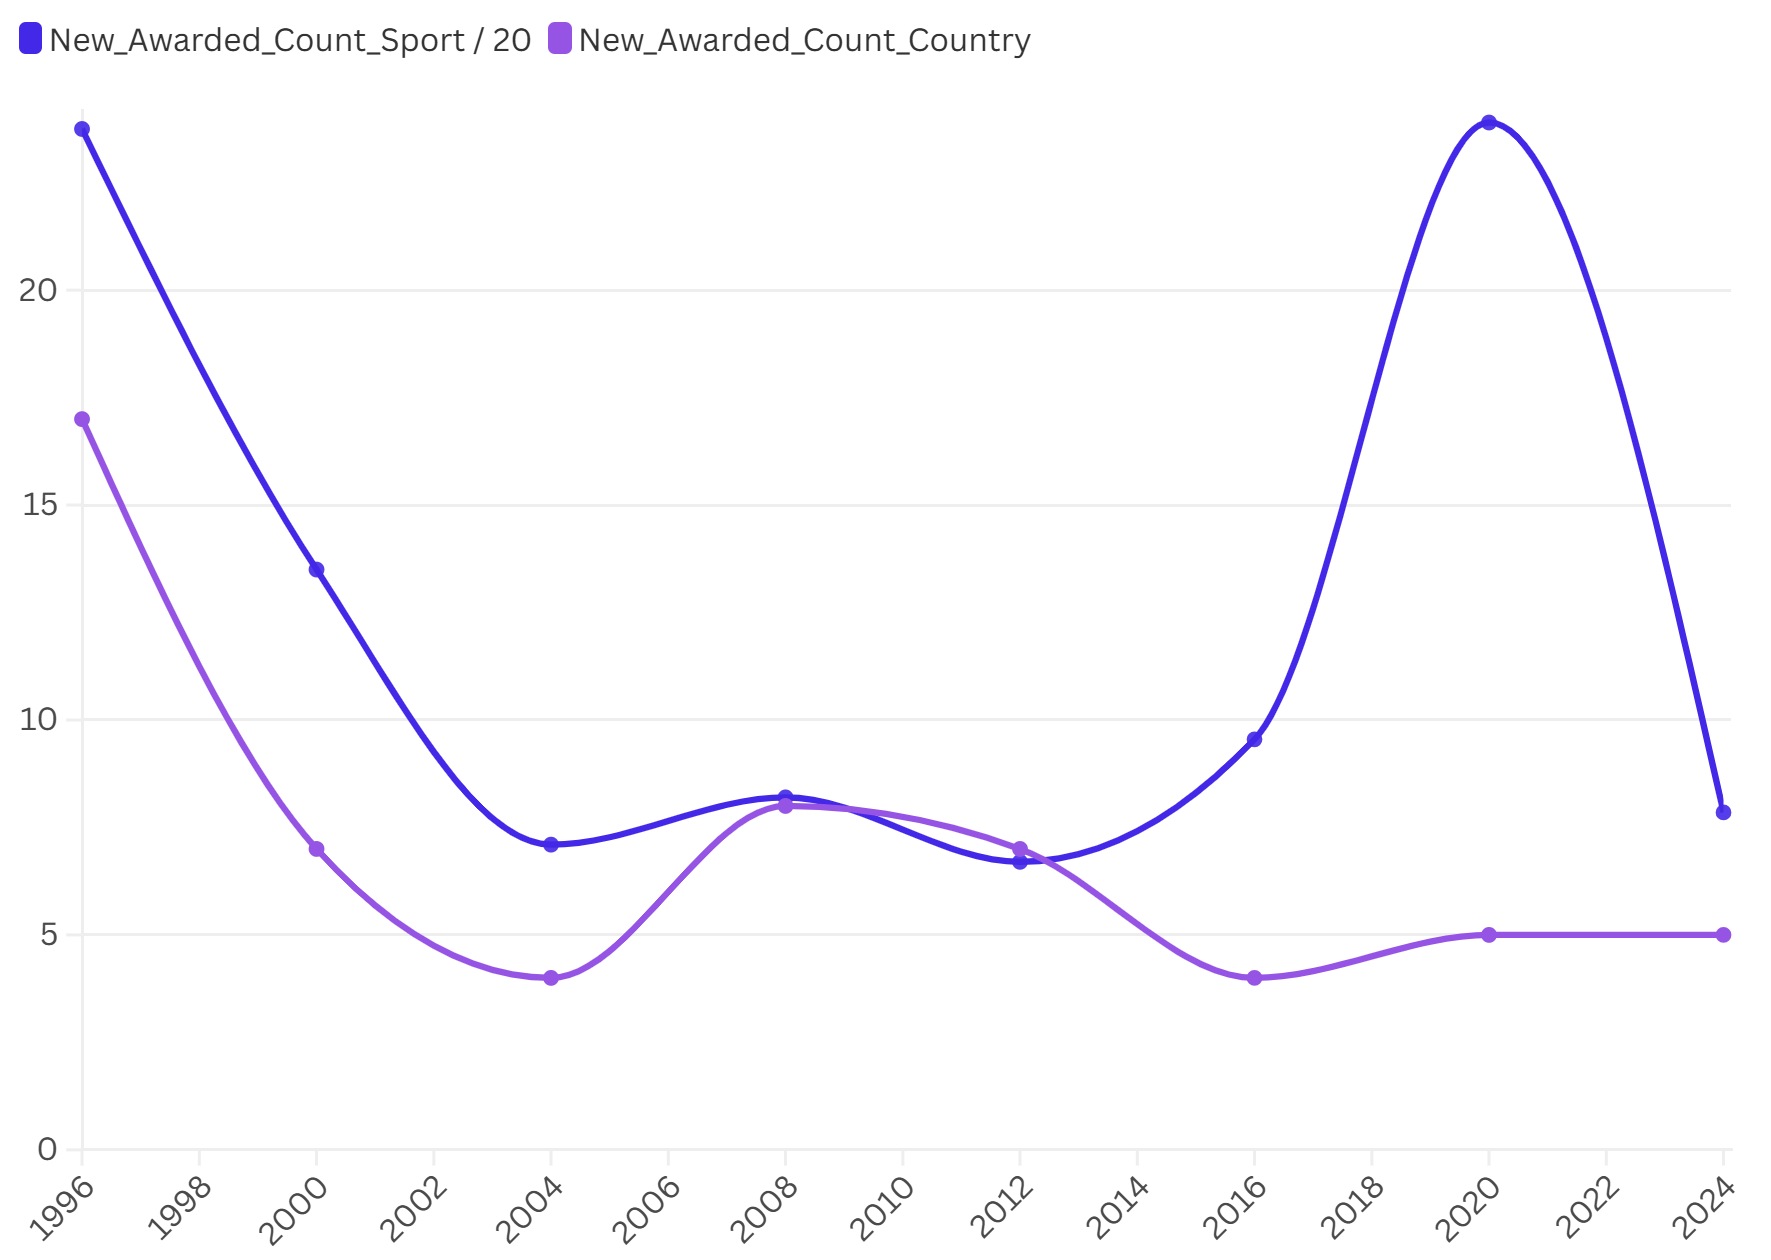
\includegraphics[width=\textwidth]{MCM2025_Latex/first medal.png}
        \caption{With 2020}
        \label{fig:The occurrence of A and B}
    \end{subfigure}
    \hfill
    \begin{subfigure}[b]{0.35\textwidth} % 调整宽度
        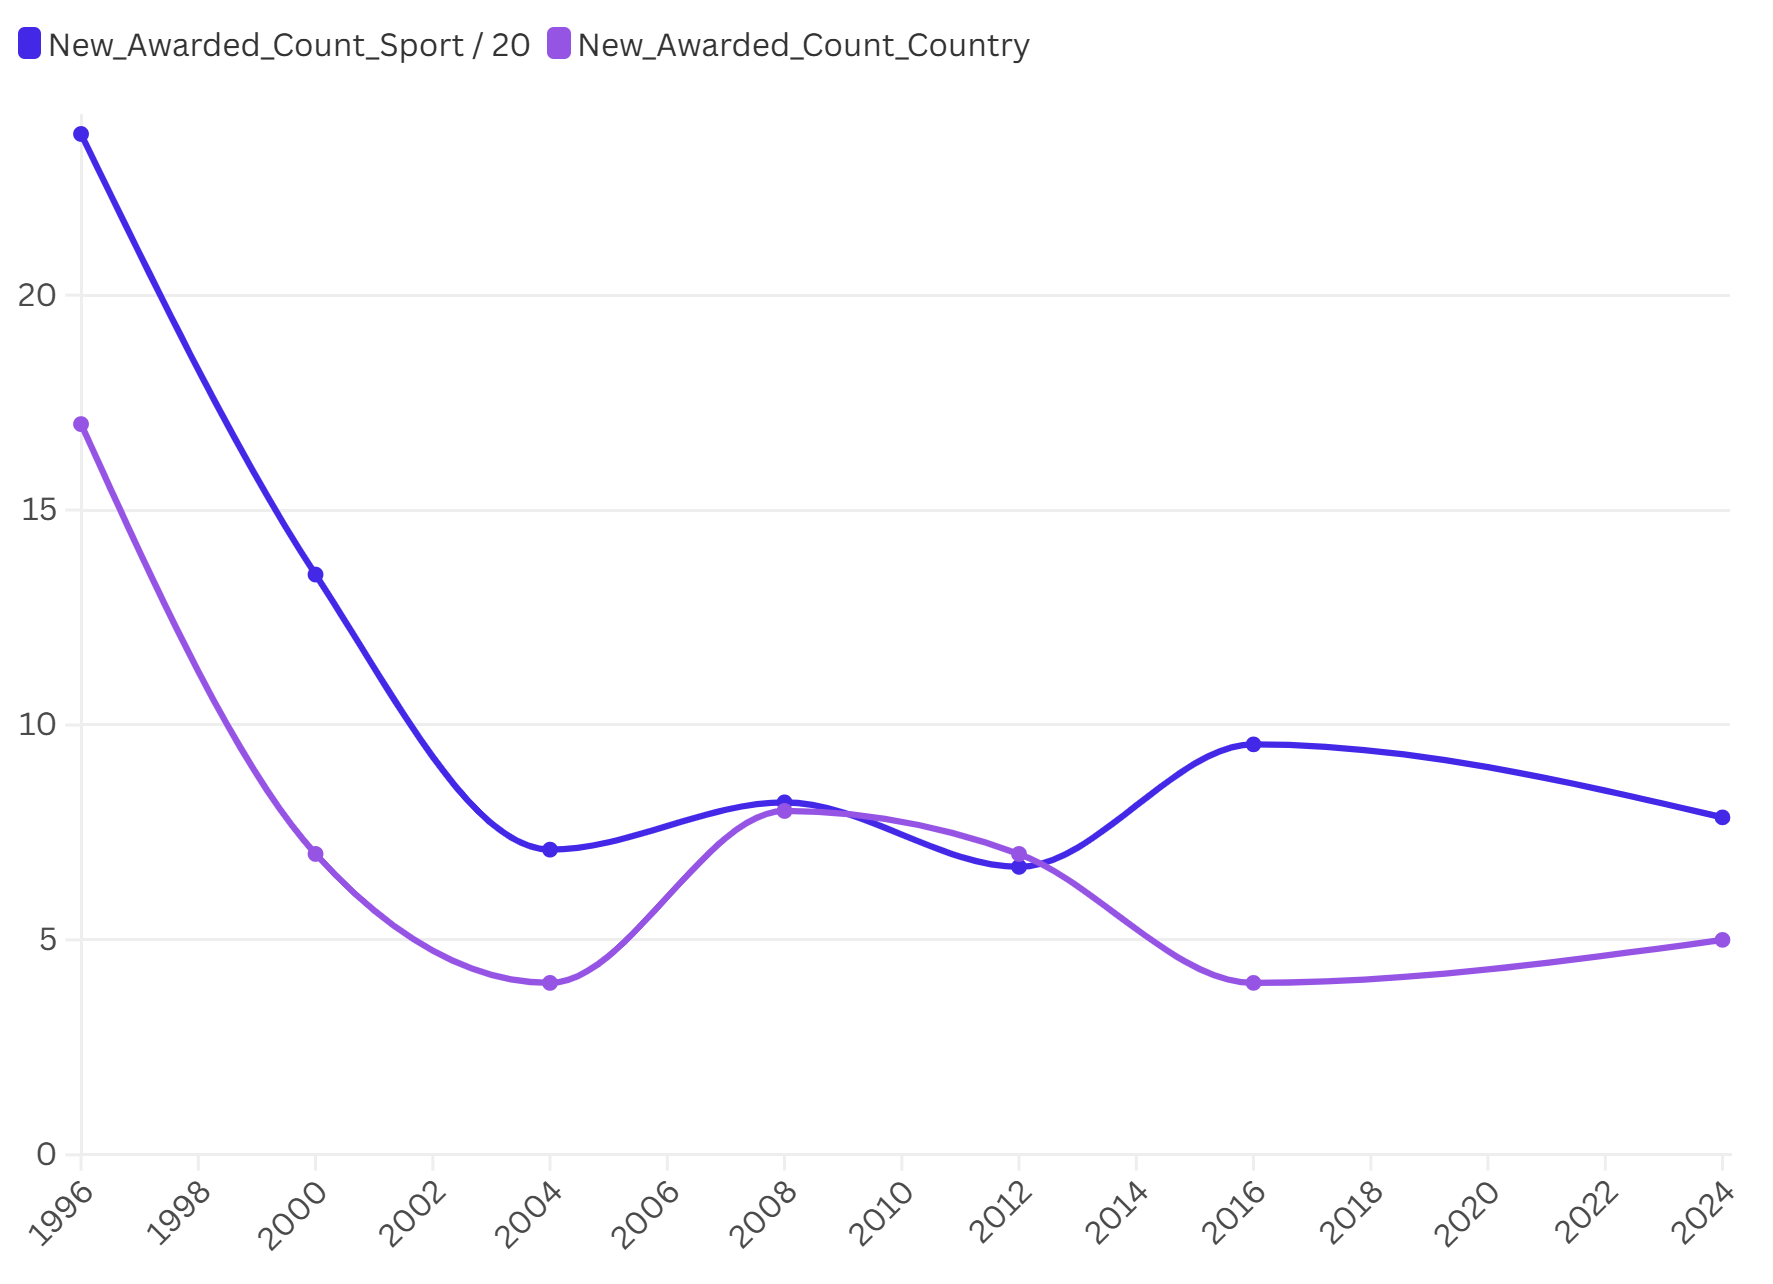
\includegraphics[width=\textwidth]{MCM2025_Latex/first medal excluding 2020.png}
        \caption{Without 2020}
        \label{fig:The occurrence of A and B without 2020}
    \end{subfigure}
    \hspace*{0.1\textwidth} % 右侧添加空白
    \caption{The occurrence of A and B.}
\end{figure}


According to our model, event $A$ attributes to two possible factors: one is the \textbf{stable improvement} of a country in one sport (event $A_1$), which can be predicted by our previous Country / Sport Gamma Model, and the other is the \textbf{random effect} (event $A_2$). Obviously, $\mathbb{E}[A_2] = \sum (\epsilon_c + \sum \epsilon_i)$. Intuitively, this expression is a steady time series and can be predicted. Since we can't judge the specific traits of this time series only by intuition, here we tried EWMA, ARIMA and LSTM~\cite{7}. We found that ARIMA fits the best. ($N(A_2) = N(A) - N(A_1)$, where $N(A_1)$ is derived from our previous model)

Once we separate these two events, we found that the $P(B|A_2)$ fits a time series model more possibly than $P(B|A)$ intuitively, and this is also proven by the results, despite the fact that the improvement is minor because the dataset is too small.

Finally, we predicted the $E[A_2]$ and the $P(B|A_2)$ of 2028. The final result $res = [\mathbb{E}[A_2] * P(B|A_2)] = [5.8452] = 6$ We are quite certain of this result as we only gets a $variance = 1.627$ when we applied the same logic to previous years.


\section{Events effect}

The type and number of specific events significantly influence a country's medal count. Indeed, as China excels in table tennis and the United States dominates in basketball, many countries have their own advantageous events, which often serve as major sources of medals. \textbf{Principal Component Analysis (PCA)}~\cite{8} is particularly suitable for calculating the correlation between events and the number of medals won by countries.

\subsection{Data Processing}

As a prerequisite for implementing PCA, dimensionality reduction is applied to the data.

\begin{itemize}
\item[\bf STEP 1] {To examine pairwise relationships between a large number of events, all events are arranged as both rows and columns in a square matrix, and \textbf{Pearson correlation coefficients} 
\[r = \frac{\text{cov}(X, Y)}{\sigma_X \sigma_Y}\]
are used to assess whether there is a linear relationship between any two events.

Based on this matrix, we find that events belonging to the same sport generally have higher correlation coefficients, which provides a basis for grouping events into sport categories for analysis.}

\item[\bf STEP 2]{We generated a table where the horizontal coordinate is the sport, the vertical coordinate is the country, and the data are the scores that each country has earned in that sport. The scores were obtained by weighting and summing the gold, silver and bronze medal awards. To determine the results of advantageous sports, we reprocessed this table by standardizing it according to sports categories using the \textbf{The z-score standardization method} as follows:
\begin{equation}
z_{ij} = \frac{x_{ij} - \mu_j}{\sigma_j}
\end{equation}
where \( \mu_j \) is the average score of event \( j \), and \( \sigma_j \) is its standard deviation.
For each country, the top ten events were selected and ranked based on their significance, identifying them as the country's advantageous events.

However, considering cases where the data values are too small (below -0.15), we argue that even if this event is relatively advantageous for the country compared to its other events, it still lacks absolute competitiveness and is unlikely to result in medal wins.

Therefore, we generated a heatmap Using ReLU function,(Fig.~\ref{fig:advantage10_compare_self}) in which data marked in blue indicate insufficient strength and are thus considered invalid, while only the data highlighted in orange are deemed effective. The heatmap suggests that most countries show limited actual performance and relatively low medal potential in their "top ten advantageous events." These countries have a relatively minor influence on our subsequent PCA analysis.

Here, we focus our analysis only on countries with a significant number of effective values. Certainly, our analysis remains applicable to others; however, prioritizing the development of their most proficient sports is likely the most effective strategy for those countries.
}

\begin{figure}[h!]
    \centering
    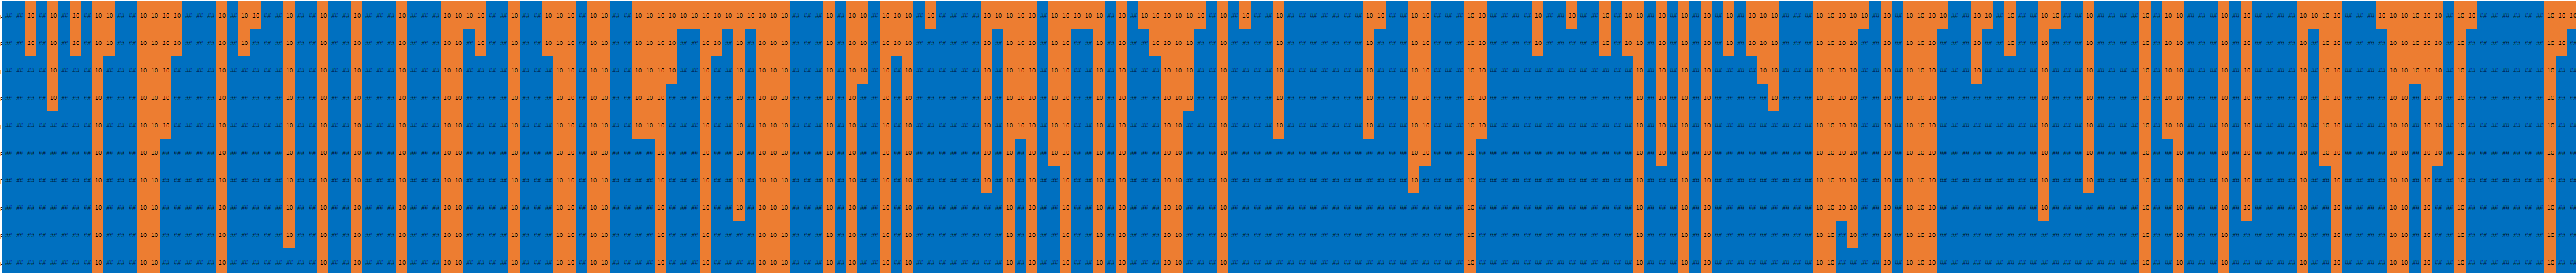
\includegraphics[width=0.8\textwidth]{advantage10_compare_self.png}
    \caption{Heatmap of Relative Competitive Strength of Countries in Different Olympic Sports}
    \label{fig:advantage10_compare_self}
\end{figure}

\end{itemize}

Through the aforementioned steps, we successfully reduced the data dimensionality to a $46 \times 74$ matrix.

\subsection{Data Analysis}
Using the z-score standardization method, the filtered $(z_{ij})$ values can be used to construct the covariance matrix of the standardized country-event score matrix $Z = (z_{ij})$ , ensuring the validity of \(\operatorname{Cov}(X) = \frac{1}{n-1} Z^T Z\), where $Z$ is the standard matrix.

Next, its eigenvalues and eigenvectors are computed. The eigenvalues represent the amount of variance explained by each principal component, while the eigenvectors indicate the direction of the principal components (i.e., the linear combination coefficients). 
Thus, we can further decompose Equation (\ref{equ:ZTZ}):\(\text{Cov}(X) = Q \Lambda Q^T\), where \( \Lambda \) is the diagonal matrix of eigenvalues, and \( Q \) is the corresponding matrix of eigenvectors.

We sorted the eigenvalues in descending order and selected the principal components that explain the largest proportion of variance. Our results are presented in the Table~\ref{tab:pca_variance} and further visualized in Fig.~\ref{fig:PCA_explained_variance_ratio}.

\begin{figure}[h!]
    \centering
    \begin{minipage}{0.35\textwidth}
        \centering
        \resizebox{\textwidth}{!}{ % 缩放表格到 minipage 的宽度
        \begin{tabular}{cc}
        \toprule
        Principal Component No. & Proportion of Variance Explained (\%) \\
        \midrule
        1 & 39.78 \\
        2 & 10.23 \\
        3 & 7.27 \\
        4 & 6.54 \\
        5 & 4.88 \\
        Cumulative 1-4 & 63.82 \\
        \bottomrule
        \end{tabular}
        }
        \caption{Proportion of Variance Explained by Principal Components}
        \label{tab:pca_variance}
    \end{minipage}
    \hfill
    \begin{minipage}{0.35\textwidth}
        \centering
        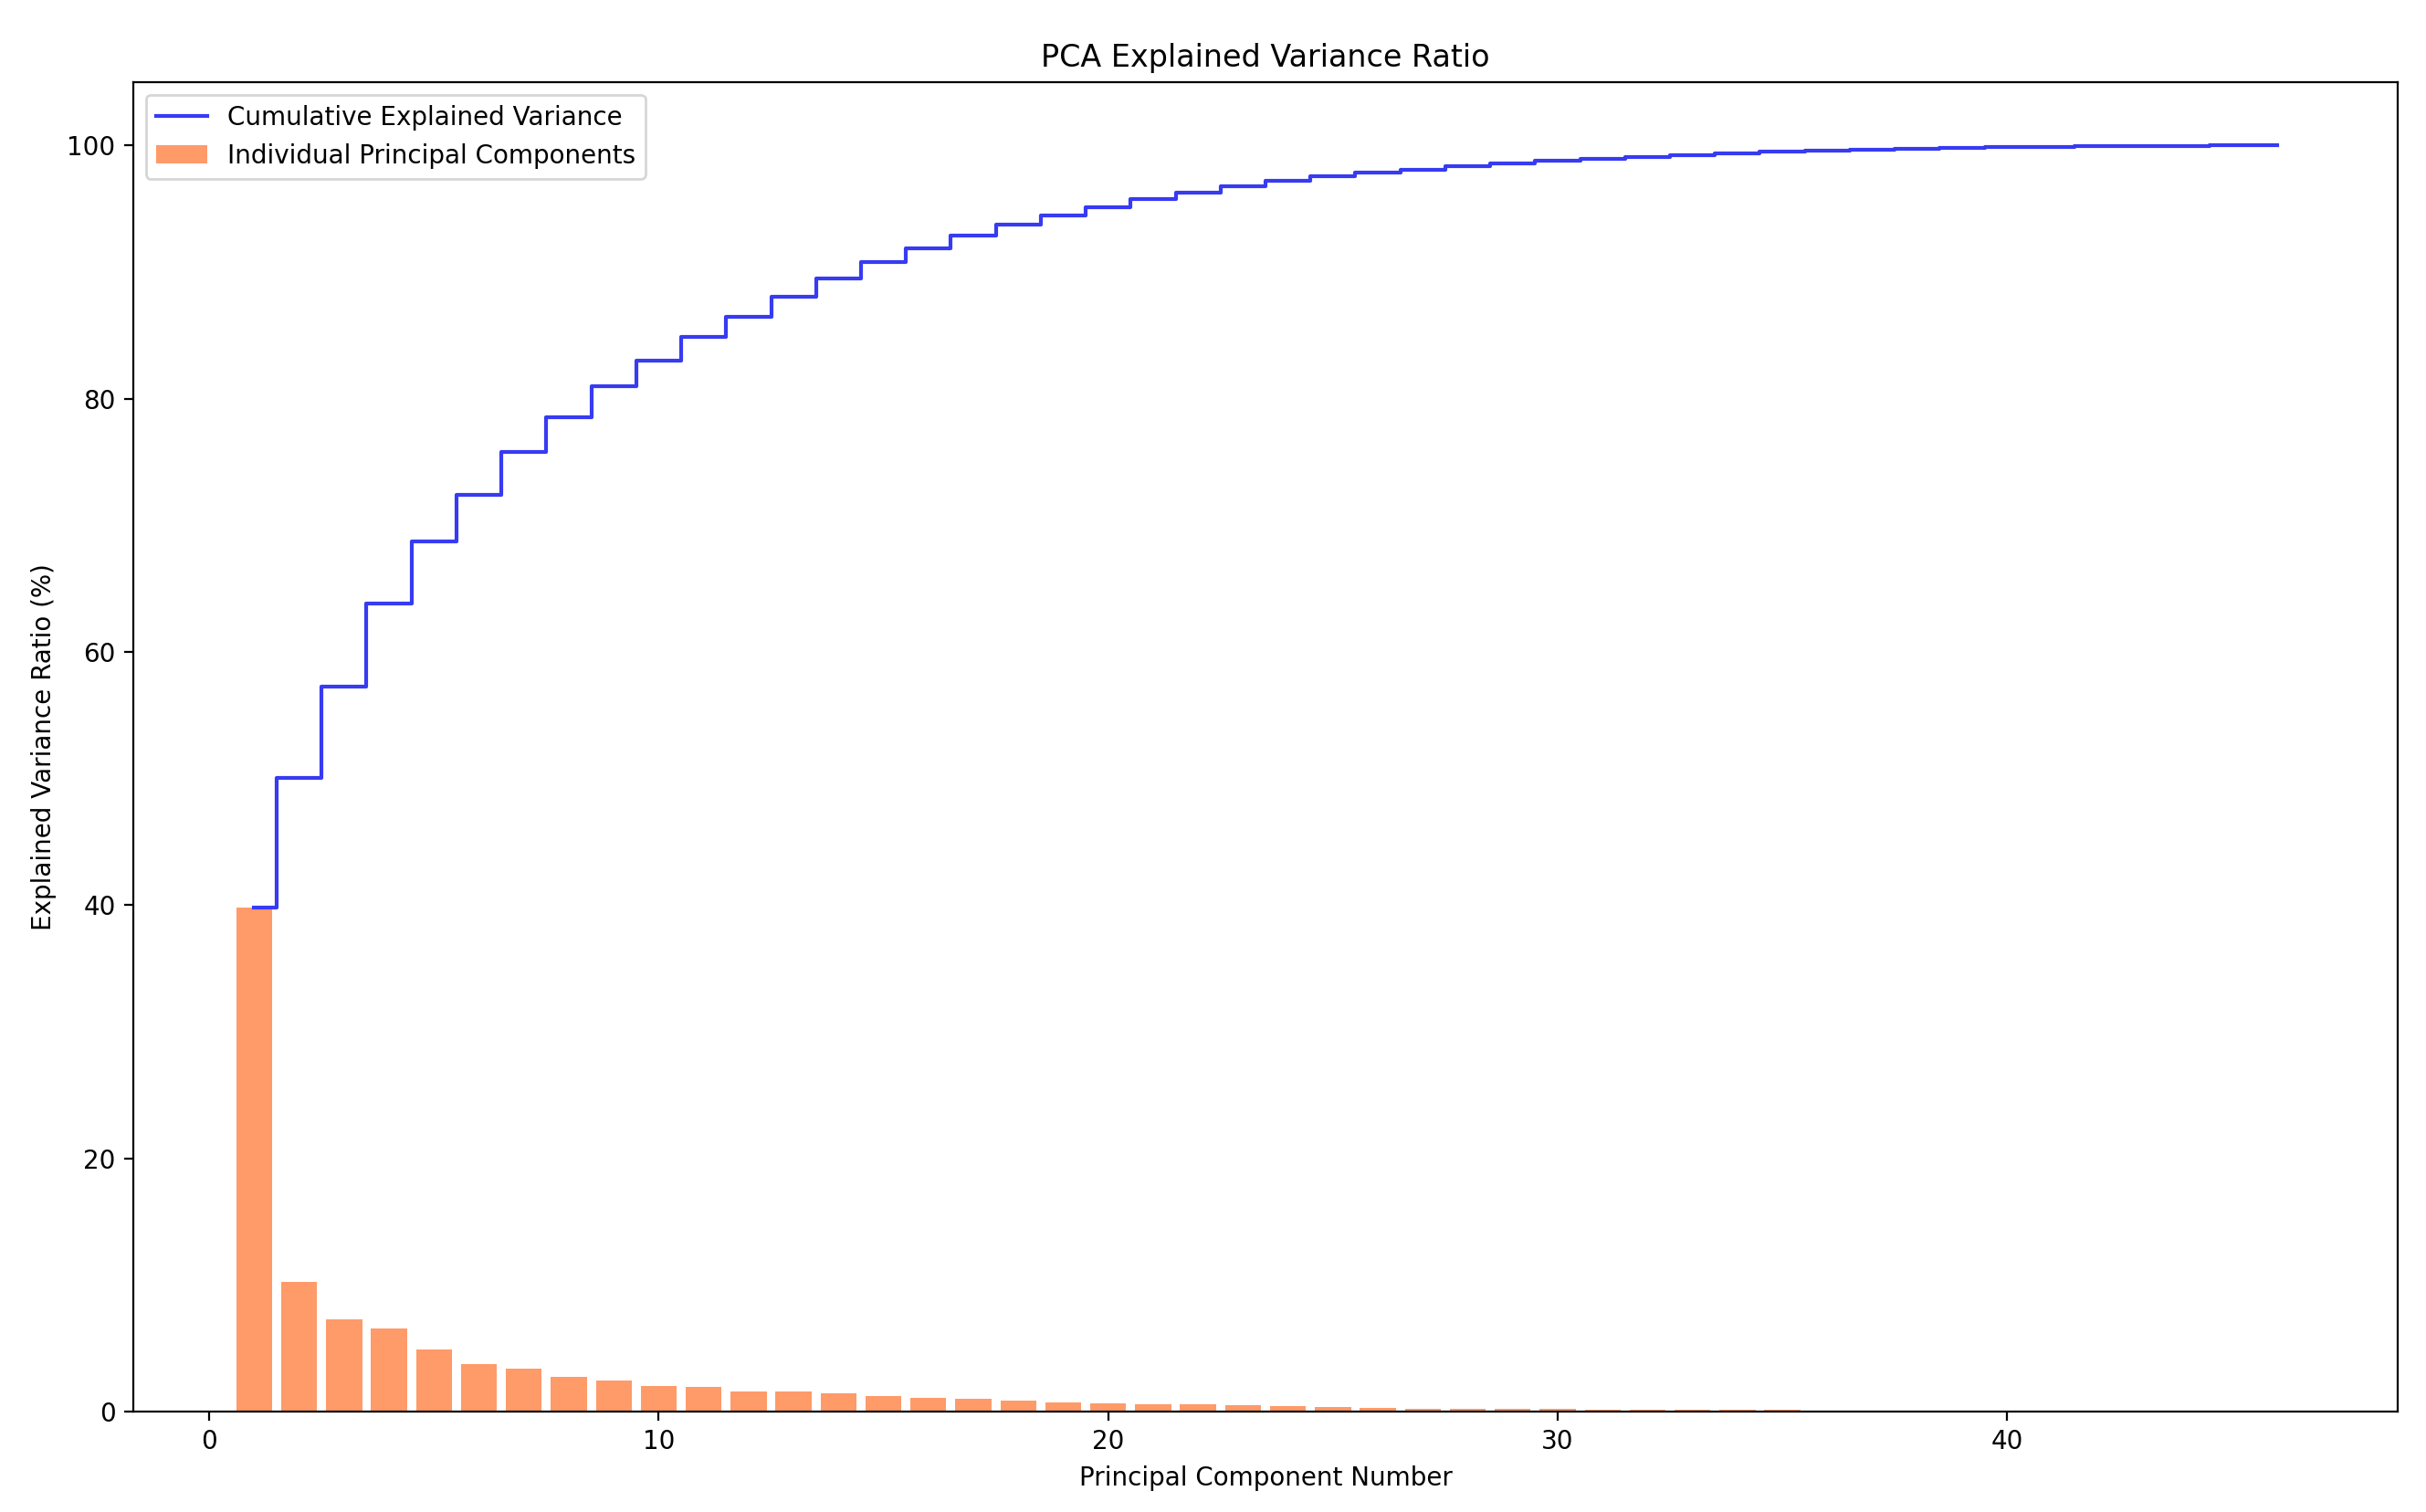
\includegraphics[width=\textwidth]{PCA_explained_variance_ratio.png}
        \caption{PCA Explained Variance Ratio}
        \label{fig:PCA_explained_variance_ratio}
    \end{minipage}
\end{figure}

%第五个及其之后的占比小于5\%,同时前四个占比之和达到了63.82\%,因此我们只看前四个特征向量。我们选择每个特征向量里影响最大的前四个因素,然后让GPT总结一下每一类的相似之处。我们发现:
From  Fig.~\ref{fig:PCA_explained_variance_ratio} and Table~\ref{tab:pca_variance}, it can be concluded that the eigenvalues ranked fifth and beyond each account for less than $5\%$ of the total variance, while the top four eigenvalues collectively explain $63.82\%$ of the variance. Therefore, we focus only on the first four eigenvectors. We selected the four most influential factors in each eigenvector and queried GPT to summarize the similarities within each category (For details, please refer to the \emph{Report on Use of AI}). Our findings are as follows:

\begin{itemize}
\item {\bf Recurrence }: There are some sports like Badminton and Artistic Swimming that appears important in different eigenvectors. They even have similar importance in different eigenvectors.
\item {\bf Similarities }: For each eigenvector, all of these sports have relatively centralized similarities. 
\item {\bf Differences }: At the same time the generalization of similarities exhibited by different eigenvectors varies。
\end{itemize}

In Fig.~\ref{fig:sports_importance_gptsummary}, we list internationally significant sports, compute the dot product of their eigenvectors with the corresponding country rows, and derive the performance of different countries across the four eigenvector categories. This allows us to identify the advantageous sports for each country. The heatmap Fig.~\ref{fig:PCA_final_heatmap} indirectly illustrates the key sports for different countries through the four eigenvector-based categories, highlighting the sports through which they achieve high scores, or favorable medal distributions. Meanwhile, the relationship between the events and how many medals countries earn.


\begin{figure}[h!]
    \centering
    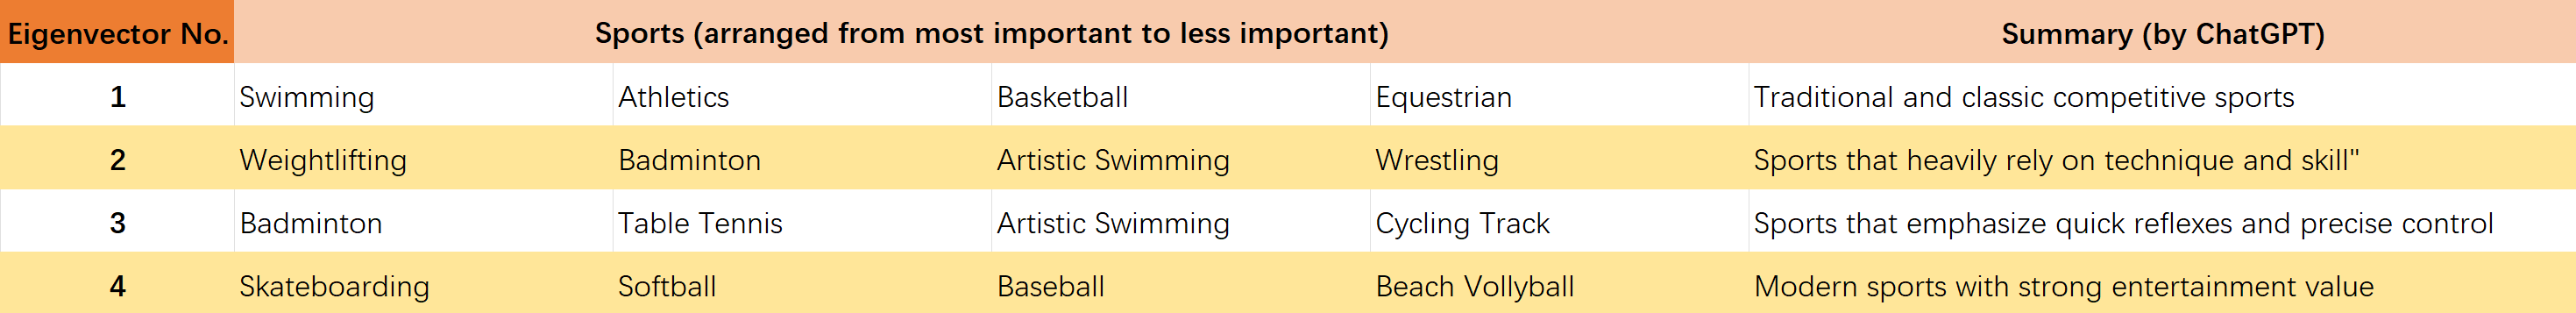
\includegraphics[width=0.8\textwidth]{sports_importance_gptsummary.png}
    \caption{PCA Explained Variance Ratio}
    \label{fig:sports_importance_gptsummary}
\end{figure}

%以上是国际上的重要运动,我们将特征向量和对应的国家所在行点乘,从而得到不通国家在这四个特征向量类上的表现情况,从而得到了不同国家的优势项目。以下热图就是不同国家各自的重要项目sport(通过四个特征向量代表的分类间接展示),通过这些项目它们能够获得很好的score,也就是获得很好的奖牌分布情况。(原文用..., the relationship between the events and how many medals countries earn. 作为结尾句。)

\begin{figure}[h!]
    \centering
    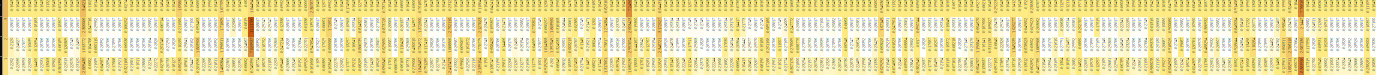
\includegraphics[width=0.8\textwidth]{PCA_final_heatmap.png}
    \caption{Heat Map of Key Sports for Different Countries}
    \label{fig:PCA_final_heatmap}
\end{figure}

\subsection{Home Country Effect Presentation}

When examining medal trends by event, we also observe that host countries can gain a competitive advantage by applying to add more events and categories in which they excel, thereby increasing their medal potential.

\begin{figure}[h!]
    \centering
    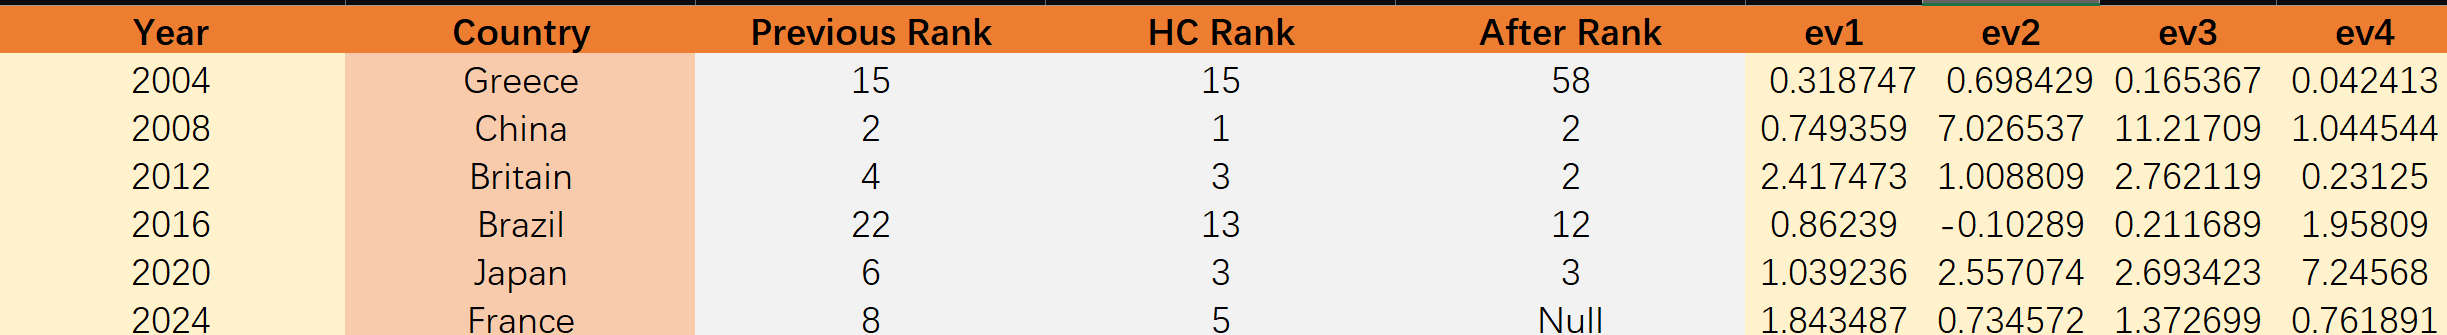
\includegraphics[width=0.8\textwidth]{HC.png}
    \caption{Home Country Effect}
    \label{fig:HC}
\end{figure}

By analyzing the data in Fig.~\ref{fig:HC}, we can draw the following conclusions:

\begin{itemize}
\item {\bf Home Country Effect DO Exist}: For all host countries, there was a notable improvement in their rankings compared to the previous year, alongside a more pronounced increase in the number of medals across each category.

\item {\bf Hierarchy}: The extent of this rise is hierarchical. For countries that were originally ranked higher, the rise in national rankings was smaller. For countries with lower rankings, the magnitude is larger. By statistically processing the actual number of awards over the years, we find that for higher rankings, the difference in strength between them is generally greater, which is a reflection of the ranking density effect. Thus the extent to which they reach a rise in rankings through the home country effect is weaker.

\item {\bf The Trailing Effect}: Each country is able to maintain its Home Country Effect relatively well in the second term as home country, continuing to perform at a high level, but returning to its original level in the second term and beyond.
\end{itemize}

Based on the relevant data, we roughly derived the following computational formula:
\[[Increase] = \sum 0.4731 \times x_i\]
This implies that the value corresponding to this country in the $i$ eigenvector equals the increase in the number of gold medals.
Moreover, since the number of silver and bronze medals is dynamically conserved, under the assumption "Medal Weight" that 1 silver medal is equivalent to 2 bronze medals, the weighted medal count can be calculated as follows:
\[[Counts] = 9.2137-2.5402 \times x_i\]

Based on calculations, the Home Country effect overall \textbf{ leads to a 16.7\% increase} in the number of medals.

The analysis above indicates that the Home Country effect primarily relates to the number of advantageous events, the performance gap between athletes, and factors such as local support and adaptation to the natural environment. Given the limitations of the dataset, the current model remains relatively crude and cannot capture detailed patterns with high accuracy. We will explore these aspects further in the concluding section of the article.

%根据相关数据,我们只能粗糙得出下面的计算式:
%\[\sum 0.4731 \times x_i\]( 第i个特征向量里面对应这个国家的值)= 金牌增加量
%银牌和铜牌动态守恒,假设银=2铜,\[9.2137-2.5402 \times x_i\]为和
%泛化来说,东道主总体上会带来16.67\%的奖牌数提升。
%实际上东道主影响涉及了东道主特长项目增加的数量多少,以及相关运动员和其他国家相关运动员的实力差距大小。这两点在目前比较难以获得准确的规律性建模,因此上述模型是极其粗糙的模型。同时东道主影响还可能体现在本土人民支持、自然环境适应度等方面,在文章最后进一步分析。

More, if some of the countries have similar advantageous items as the host country (which can be simulated by our PCA method), then we can say that these countries will also be favored by the home country effect. As analyzed in the previous data, no two countries have exactly the same advantageous items, so this favor is weaker than the host itself, similar to a differential mode.

\section{Great Coach Effect}
\label{sec:6}

During our earlier analysis of the model, we realized that it is not entirely complete, and certain additional factors could affect the prediction results. Next, we will delve into the influence of the "Great Coach" factor.

\subsection{Evidence Search}

To identify evidence of changes that might be attributed to the "great coach" effect, we start with the \textbf{definition of the great coach effect}: a great coach enables the same team or athletes to achieve significant success. Given the four-year interval between Olympic Games, we assume that a coach deemed great can lead the team to substantial breakthroughs within this period, reflected in a notable improvement in medal outcomes.

Therefore, we employ a time-series \textbf{differencing method}. We first calculate a weighted sum of medal counts to derive a score, then compute the first-order difference of this score over time, and divide it by the number of participants. This process yields the following statistical data in Fig.~\ref{fig:coach_abs_score_change}, with two points worth noting:
%为了找到evidence of changes that might be due to a “great coach” effect,我们从great coach effect的定义出发:因为一个伟大的教练而使得相同的团队或运动员达到巨大成功。由于奥运会四年一次的长间隔,我们假设足以称为伟大的教练能够在四年里带领队伍达成较大的突破,体现在成绩上则是较大的获奖情况的改观。因此我们首先对于奖牌数量进行加权相加得到score,然后对于score按照时间进行一级差分,除以参赛人数,得到了下面的统计数据:

\begin{figure}[h!]
    \centering
    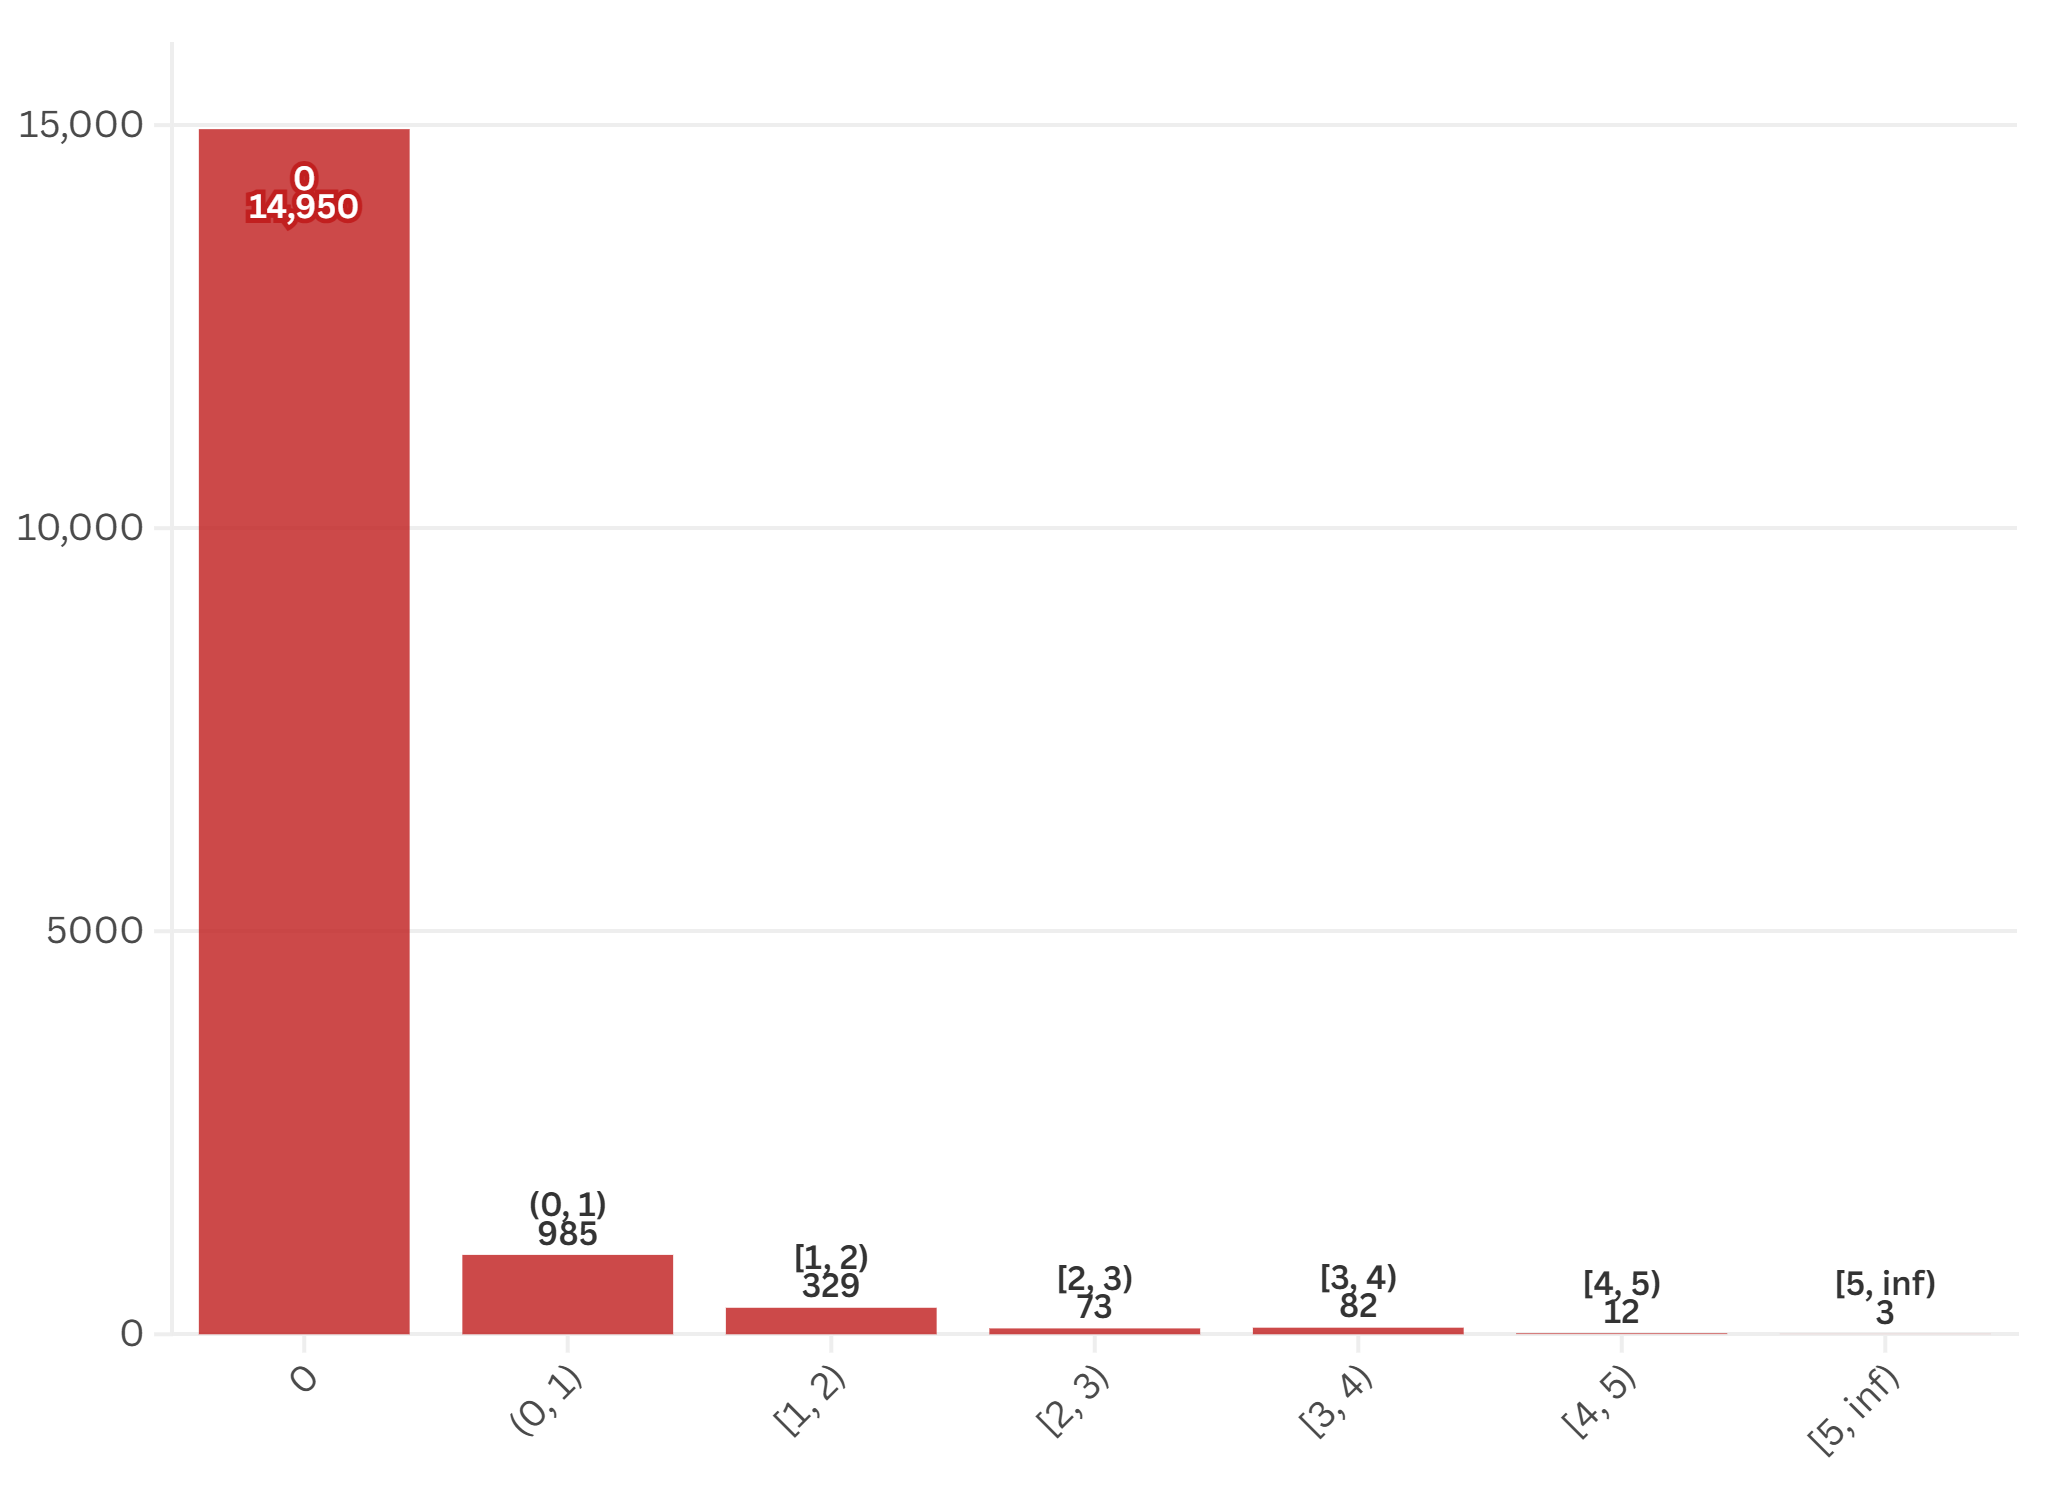
\includegraphics[width=0.4
    \textwidth]{coach_abs_score_change.png}
    \caption{Absolute value of first-order differences in scores for the same country and sport}
    \label{fig:coach_abs_score_change}
\end{figure}

%%!!!!!assumption被改了,这里要改掉写法--------|v|---------
\begin{itemize}
    \item[1)] Here we used the weights of [16,4,2,1] instead of [8,4,2,1] weights in the assumptions to more prominently highlight the significance of winning gold medals, and thereby making potential evidence of great coach effects more apparent.
    \item[2)] Based on data analysis, we find that great coaches like Lang Ping\cite{3} and Béla Károly\cite{4} have a similar impact on all events within a sport category. This provides a rationale for dimensionality reduction, allowing us to analyze each country's performance at the sport level.
\end{itemize}
%注意,1。 在这里我使用了[16, 4, 2, 1]的权重,为了更加突出地表现获得金牌这一事件,从而使得潜在的great coach event evidence能够更为突出。
%2、 通过 Lang Ping, Béla Károlyi (这里要从题目里面搞引用!!!!!!!!)<-(?)的例子,我们分析得到伟大教练会对一个sport大类的所有event都有影响。因此这里使用的是sport,进行了数据降维。

Based on our real-life experiences, we recognize that great coaches are rare, and their presence or absence usually leads to a sustained impact. Therefore, we set a threshold of 4 for the score differencing values to filter the data. When analyzing the filtered result, we found that some countries exhibit a two-year alternating high score differences in certain sports, with the magnitude of these differences being similar or identical. Through an analysis of overall trends, we conclude that these fluctuations are likely due to transient anomalous factors in the country's performance in that sport, rather than the influence of a great coach.

After a second round of data cleaning, we compare our findings with real-world data and arrive at the following analysis map for the success rate of identifying great-coach effects (Fig.~\ref{fig:coach_effect}):
%由于 great coach 的稀缺性,我们选择对于数量较少的进行进一步处理。这里选择大于等于4的进行整理。我们又发现,有些国家的项目可能存在连续两年score变化幅度很大,绝对值相近或相同,且符号相反。我们经过对于整体发展的趋势分析,认定这是其他异常的出现导致的短暂性波动,而不是coach effect带来的本应是持续性的影响,剔除了这些数据。之后我们和现实情况进行比对,形成了这样的great coach effect判断成功分析图:

\begin{figure}[h!]
    \centering
    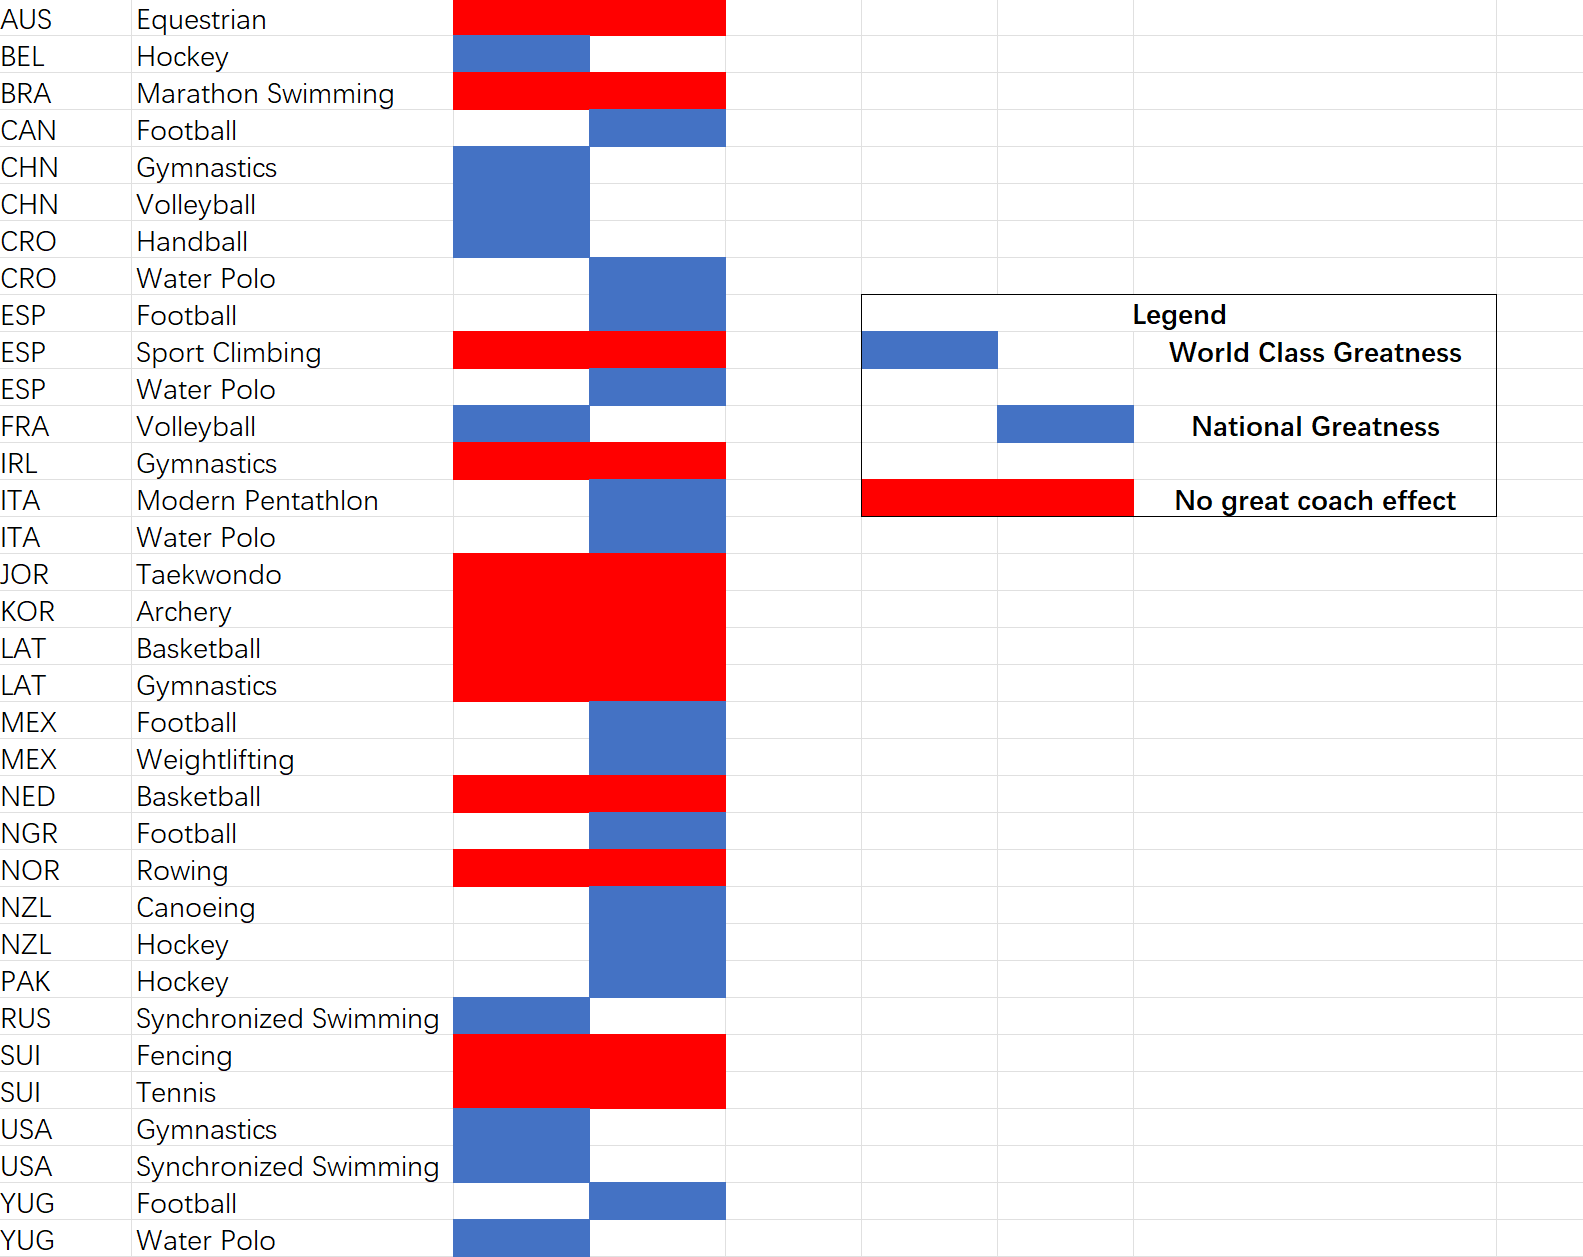
\includegraphics[width=0.4\textwidth]{coach_effect.png}
    \caption{Great Coach Effect Judgment Success Analysis Chart}
    \label{fig:coach_effect}
\end{figure}

We categorise great coaches into two levels: world level and national level. World-level coaches are those who have achieved widespread success in coaching and are recognised globally, while national-level coaches are those who have significantly advanced the sport especially in their country and gained national recognition. Our method achieves a 65\% accuracy, while all the world-class great coaches (actually limited in number) is well reflected in our results. This shows that the data for evidence of changes that might be due to a “great coach” effect selected by our method is sufficiently robust.
%我们将great coach 分为世界级和国家级,世界级是获得了世界认可的教练,国家级是为这个国家的这项运动带来了巨大提升的教练、获得国内认可的教练。我们达到了65\%accuracy。同时世界级的伟大教练本身较少,都能在这里体现出来。可见我们方法所选出的the data for evidence of changes that might be due to a “great coach” effect 足够优秀


\subsection{Impact Estimation}

We calculate the extent to which such an effect contributes to medal counts and \textbf{great coach effect (GCE)} impact with this formula:
%我们通过这个式子算出such an effect contributes to medal counts的程度,及 GCE impact:
\[
[Effect]=[GreatCoachIndex] \times [EventCounts] \times [ShiftSpace]
\]
%伟大教练指标*项目event数量*上升空间

We present our result in Fig.~\ref{fig:coach_impact} , which indicates that:
\begin{itemize}
    \item The impact of a great coach at the world-level great coach is highly significant.
    \item The impact of a great coach at the national-level is relatively less significant than that at the world-level. However, for specific countries, they have shown outstanding effects, even comparable to those of world-class great coaches.
\end{itemize}

By incorporating this GCE analysis, we improve our model, making it more precise and improving the accuracy of future medal distribution predictions.
%可以看到:(下面用分点符号)
%- 是伟大教练的影响式显著的。
%- 民族英雄相对世界伟大级别来说会弱一点,但对于特定国家而言可能会有特别突出的、和世界级的齐平的效果。

%这个GCE分析可以加入模型,更加精确化我们的建模和对于未来奖牌分布的预测。

\begin{figure}[h!]
    \centering
    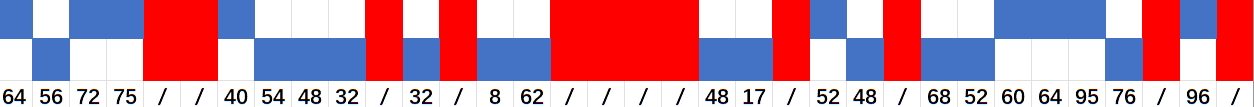
\includegraphics[width=0.6\textwidth]{coach_impact.png}
    \caption{Great Coach Effect Impact Analysis Chart}
    \label{fig:coach_impact}
\end{figure}


\subsection{Result Application}

In order to select three countries and estimate the impact of investing in a great coach, we evaluate the cost-effectiveness of this investment and quantitatively analyze its components using the model established above.
We will analyze the issue from both the outcome and cost perspectives.

\begin{itemize}
    \item {\bf Outcomes}. According to the model above, the outcome can be divided into two components: the change in the country's strength in the sport category and the number of events in that sport. While the number of events may vary by year and host country's choices, it generally follows a stable distribution and has a clear interpretation. In contrast, quantifying "changes in strength" is more complex, and we define it as follows:
    \[
    Outcome = potential \times EventCounts
    \]
    The potential can be estimated using the model we previously established through the Country / Sport Gamma function, the size of the ratio between the number of awards and the number of participants will also be one of the considerations for potentials. When we observe that the parameters of the Gamma curves for most events in two countries are similar, we can reasonably conclude that the overall levels of the two countries are comparable. Consequently, these few events may hold significant potential.
    On the other hand, the $\alpha$ and $a_{max}$ of a certain Country / Sport Gamma function can directly reflect a country's potential. For example, if a Country / Sport Gamma function has small $\alpha$ and large $a_{max}$, it means that the athletes of this country of this sport have large potential and are yet to be tapped.
    
    
    \item {\bf Costs}. It represents the financial cost required for the country to recruit the great coach, which we assume to have a near-linear relationship with the ratio of the GDP of the coach's home country to that of the hiring country. Additionally, based on researches (For example, Xun's~\cite{9}) , GDP is strongly correlated with overall medal counts, allowing us to derive an expression for cost using the given dataset.
    \[
    GDP \propto f(MedalCounts)
    \]
    
\end{itemize}

In summary of the two perspectives, the cost-effectiveness (denoted as Merit here) can be calculated using the following formula:
\[
[Merit] = \frac{Outcome}{GDP} = \alpha \times \frac{Potential \times EventCounts}{f(MedalCounts)}
\]

where $\alpha$ is a pending coefficient, $f(MedalCount)$ is a function related with medal counts. As for the selection of three countries to estimate, we choose:
\begin{itemize}
    \item {\bf Canada (CAN) investing in a great coach for fencing}. 
    Based on the model simulation, investing in this program (e.g., hiring a coach from Italy) could increase the potential by 23.5\%, indicating highly favorable cost-effectiveness.
    \item {\bf New Zealand (NZL) investing in a great coach for swimming}. 
     Based on the model simulation, investing in swimming (e.g., hiring a coach from the United States) could increase the potential by 5.1\%, indicating moderately cost-effectiveness.
     \item {\bf Australia (AUS) investing in a great coach for gymnastics}. 
     Based on the model simulation, investing in this program (e.g., hiring a coach from Denmark) could increase the potential by 9.8\%, demonstrating relatively high cost-effectiveness.
\end{itemize}



\section{Other Discovery}
\label{sec:8}

In Section 4.1, when we are calculating Gamma Loss, we spotted some athletes with abnormally high loss which is up to 18.655. 

In Section 4.2, we compared some year's predicted country's Gamma model and true Gamma model and looked into the reason why a few country received a considerable unexpected boost in certain sport.\\

\subsection{Monopoly of the Big Countries}

During the first period of data analysis, we noticed the distribution of medals is imbalanced. The top 15 countries accounted for 65.45 \% of the medals and 72.56 \% of the gold medals, as we can see in the figure. It is clear that the big countries often have a monopoly on winning medals and remain stable in their performance.

Therefore, the Olympic committees can focus on obtaining the number of athletes from large countries as well as largely increasing the number of athletes from small countries. This may add possibilities for the small countries to win medals from the big ones, reducing the monopoly of the big countries.

\begin{figure}
    \centering
        \begin{subfigure}[b]{0.4\textwidth}
        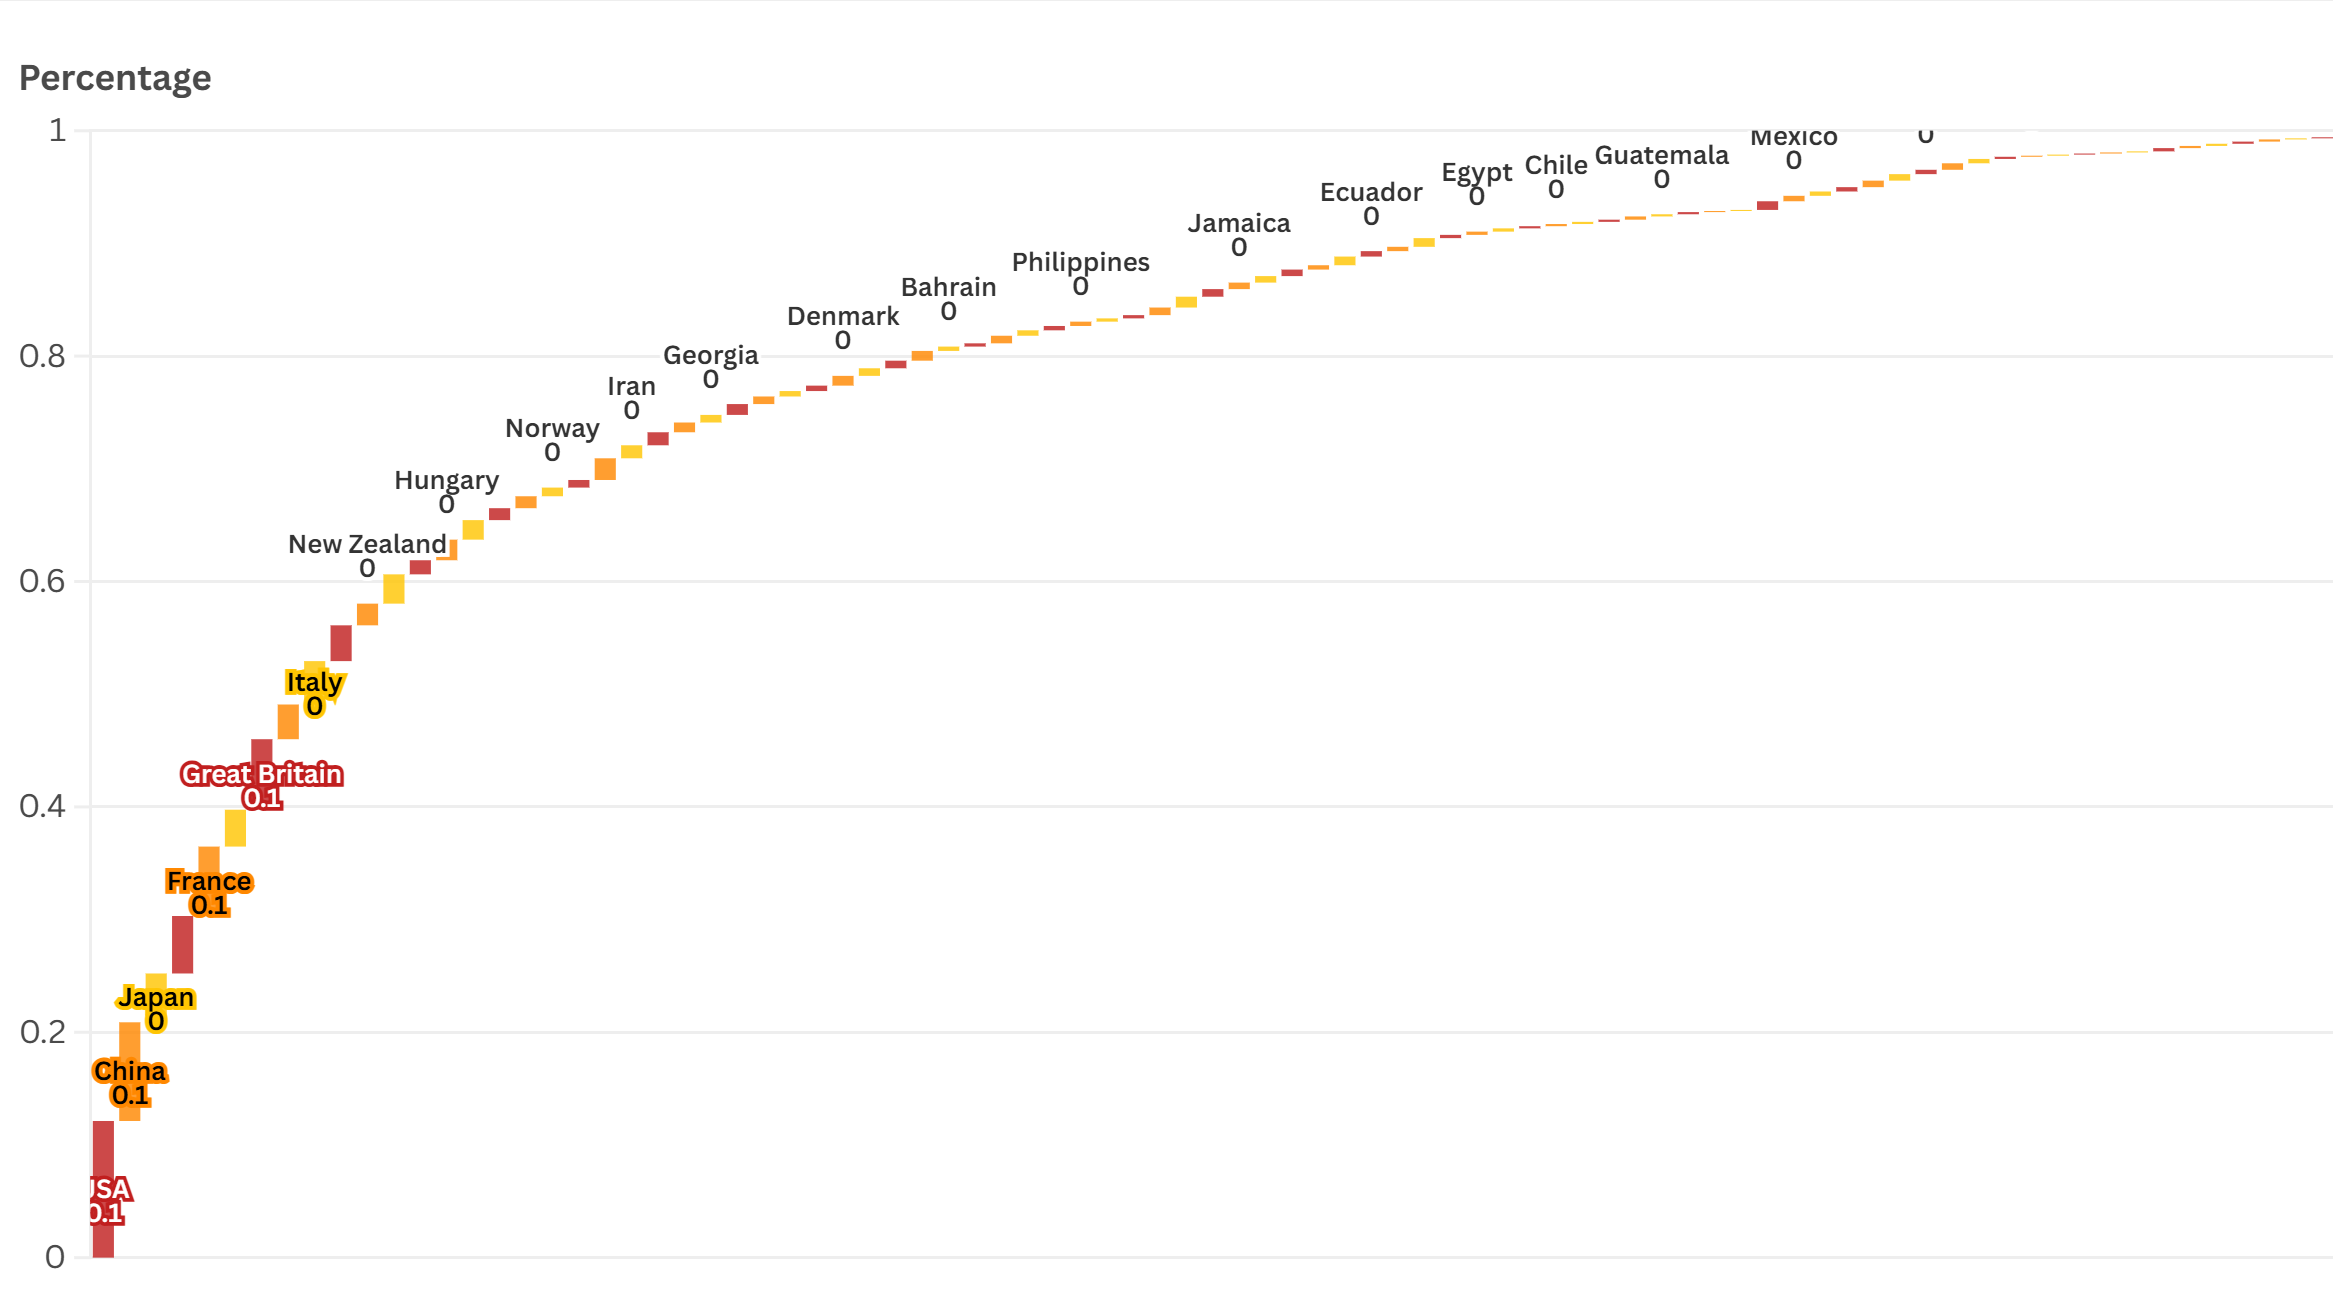
\includegraphics[width=\textwidth]{1total_distribution.png}
        \caption{Total Medal}
        \label{fig:1total_distribution}
    \end{subfigure}
    \hfill
    \begin{subfigure}[b]{0.4\textwidth}
        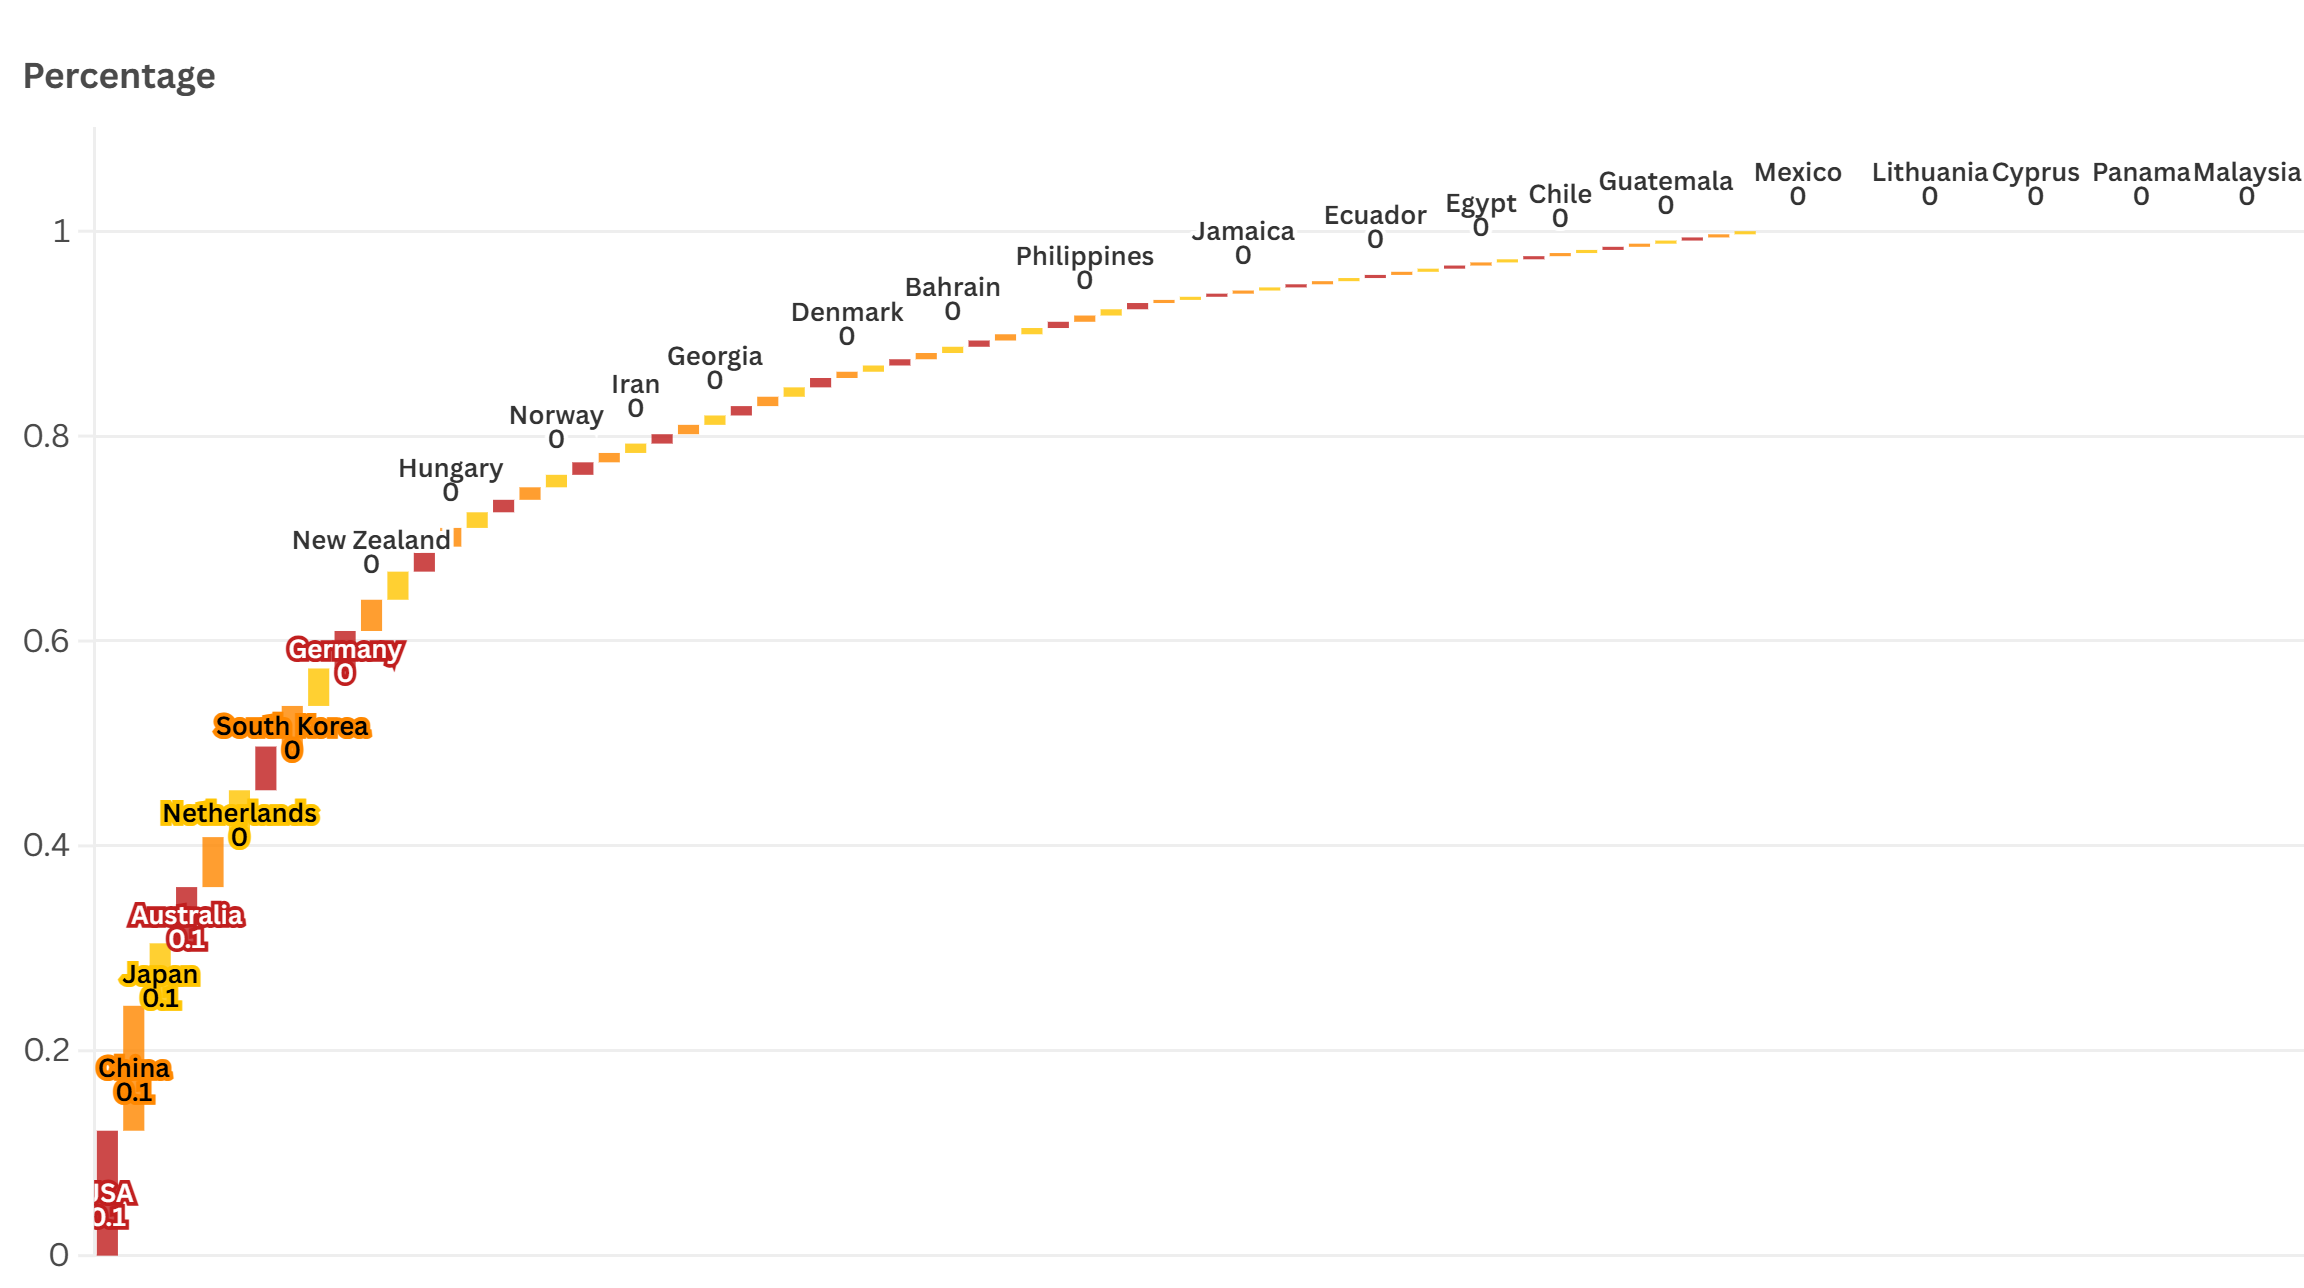
\includegraphics[width=\textwidth]{1gold_distribution.png}
        \caption{Gold Medal}
        \label{fig:1gold_distribution}
    \end{subfigure}
    \caption{Country Occupation Percentage of Total Medal and Gold Medal}
\end{figure}

\subsection{Sudden Injuries}
One abnormal value is "Sara Kolak F, Croatia, Athletics Athletics Women's Javelin Throw Gold"\cite{10}. We find out that she's actually an excellent javelin thrower, but her strength has been greatly affected by injuries. Therefore, sudden injuries is a large error that needs attention and correction. 

Unfortunately, because of the way our model is designed and the training data we've got, we can't yet accurately predict this factor. So, at the moment, we can only guess that athletes are developing steadily. To improve this, we're going to keep a closer eye on athletes' daily training and performance in the next competition, so we can reduce the impact of sudden changes in data due to injuries and illnesses.

The Olympic Committee should also endeavour to minimise permanent injuries caused by accidents during the Olympics. In addition, the Committee should present the public with more exciting competitions by enhancing attention and protection of athletes' safety。

\subsection{Geographical Differences}
When dealing with important sports in different countries in PCA, we found that for different classes of sports exhibited by the eigenvectors, the distribution of countries that specialise in them has certain geographical characteristics. For example, Europe and America are better at team ball sports (football...), and Asia is better at fast reaction and precise control sports (badminton, table tennis...).

In particular, the inclusion of a predictive model as a patch can be done by this Eq:\(\Delta n_{medal\_geo\_effect} = p_0 \times \Gamma_{geo}\)where \(p_0\) is the worldwide average performance, and \(\Gamma_{geo}\) is the geographical difference coefficient.

The total number of Olympic medals is shown in the Figure 22. We also found that most of the high number of awards are distributed in the northern hemisphere, while there is less distribution near the equator and more distribution in temperate and subarctic countries, among other geographical characteristics. It can be seen that the geographical characteristics of a country also affect the ceiling of different sports in a country and the development of native athletes.

The Olympic Committee should also make sure that there is a balance in the number of different types of events, and that the overall competition is similar for different countries. This will make sure that being excellent in some events does not have a big effect on the final result. This will make sure that the competition is fair, reasonable and exciting.

\begin{figure}[htbp]
    \centering
    \begin{minipage}{0.48\textwidth}
        \centering
        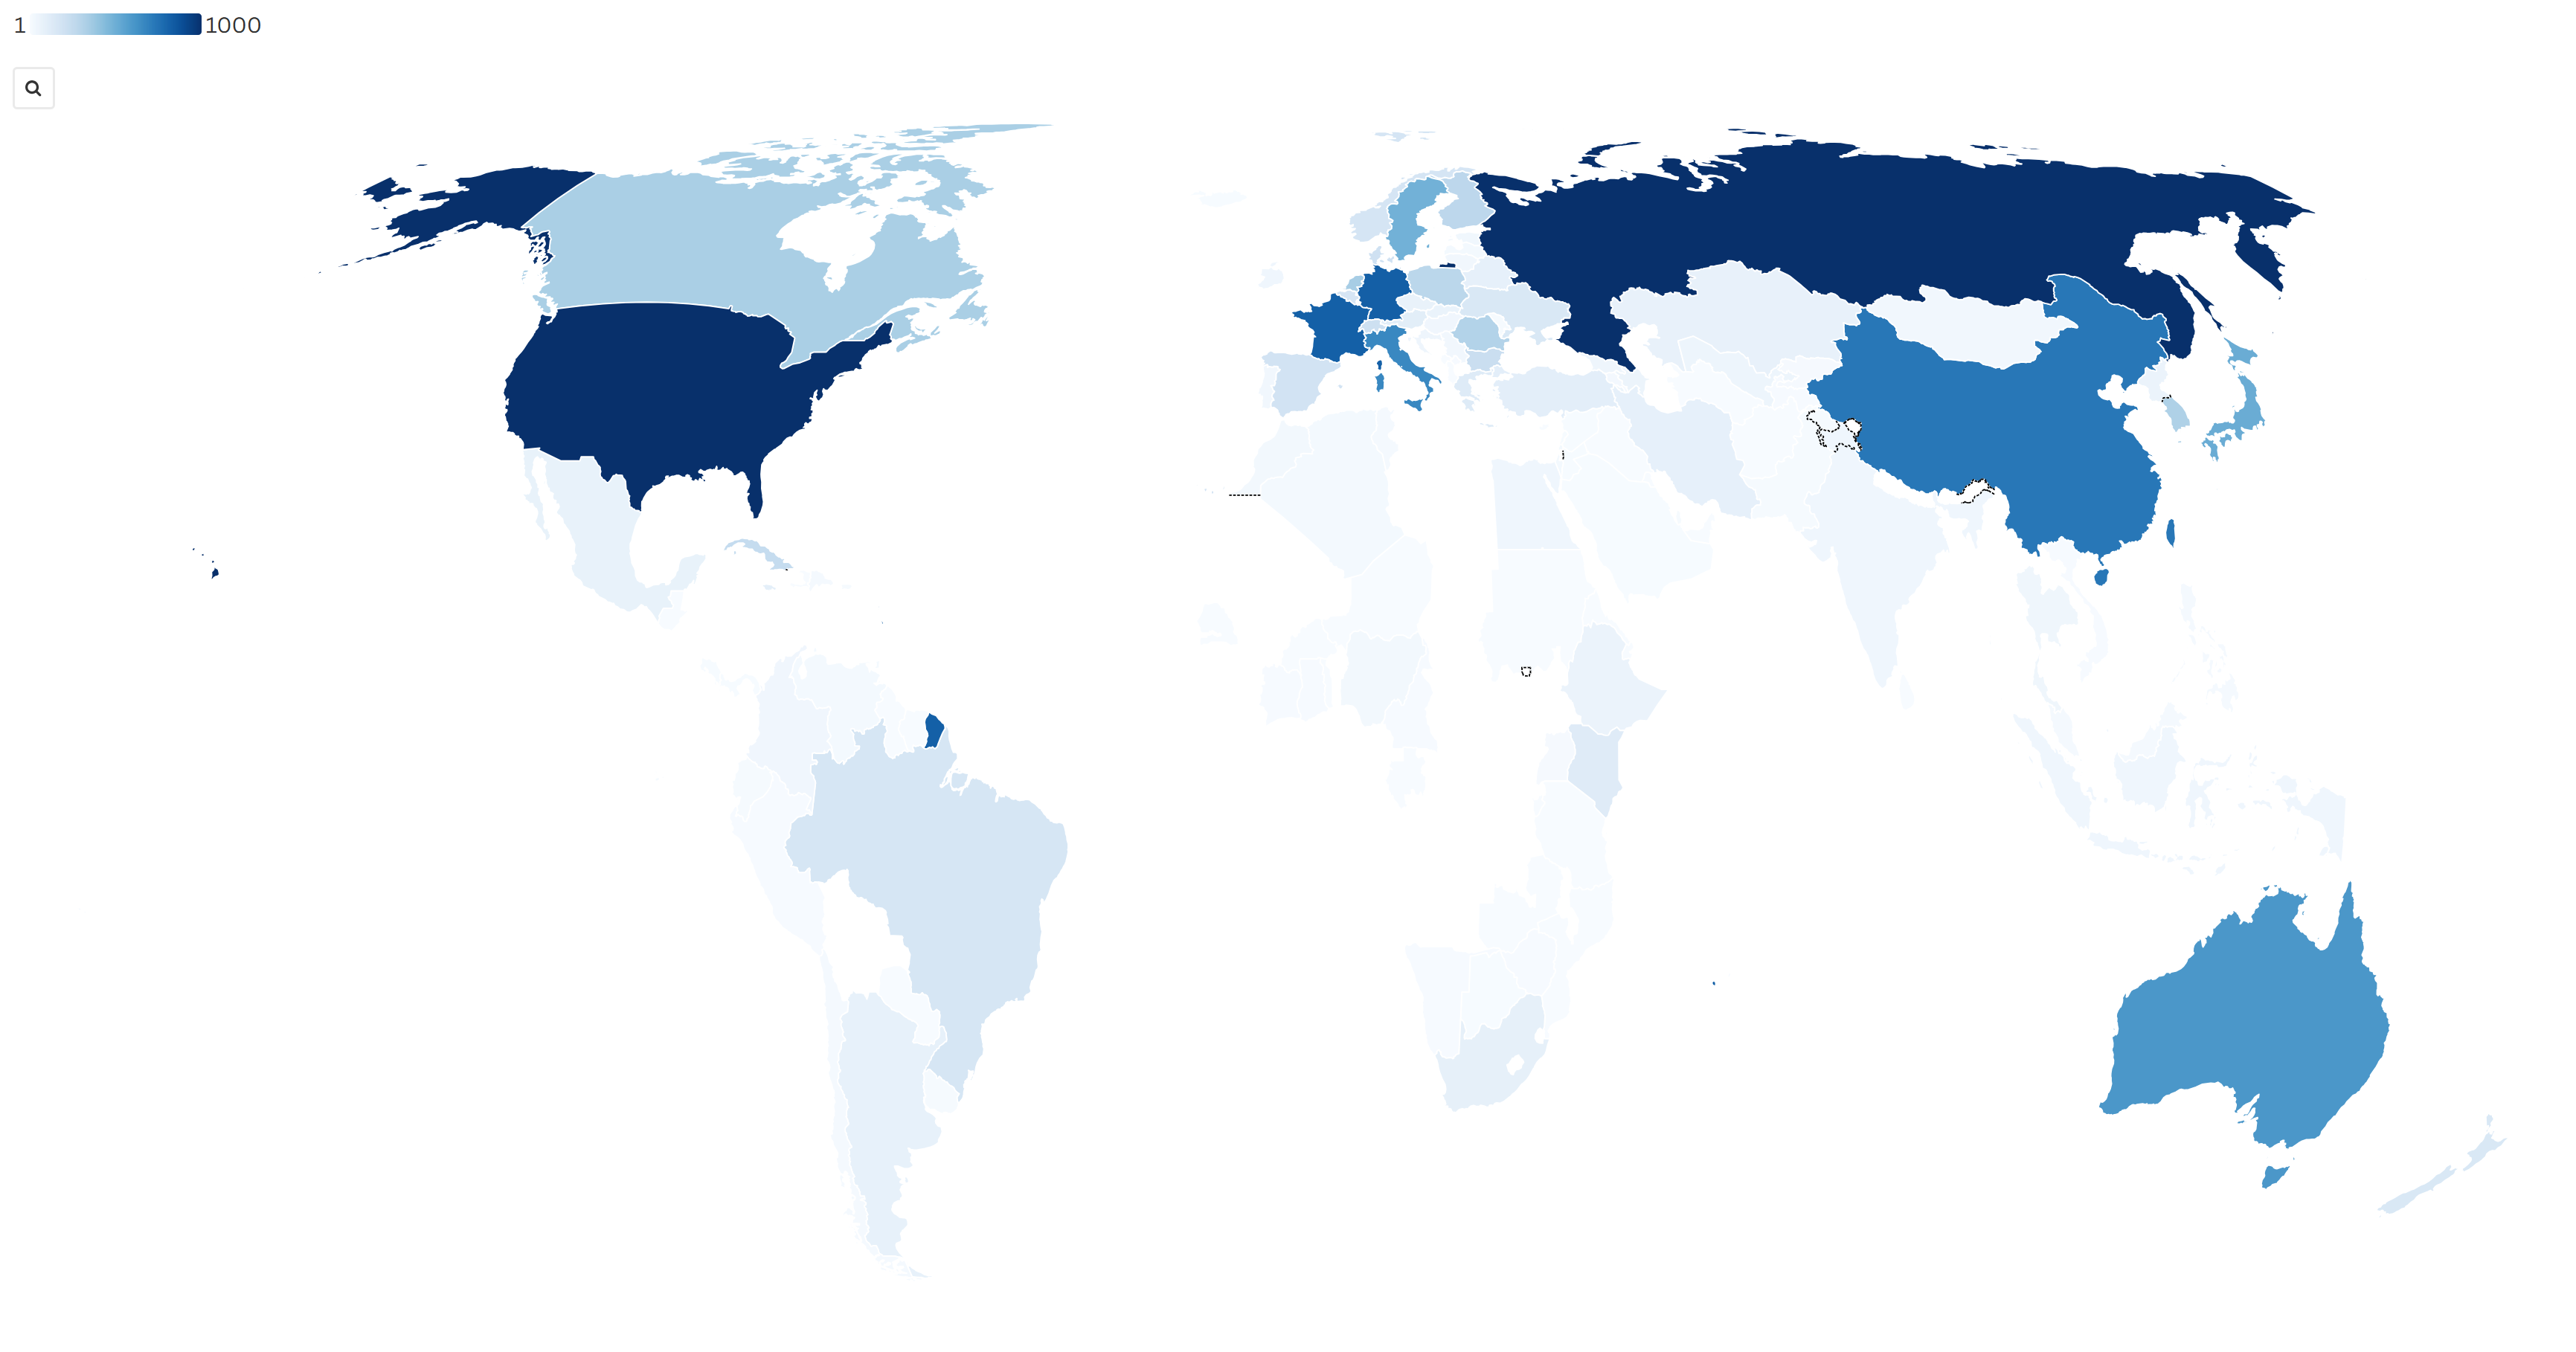
\includegraphics[width=\linewidth]{MCM2025_Latex/figures/worldmap_colored.png}
        \caption{Heatmap of Relative Competitive Strength of Countries in Different Olympic Sports}
        \label{fig:worldmap}
    \end{minipage}
    \hfill
    \begin{minipage}{0.48\textwidth}
        \centering
        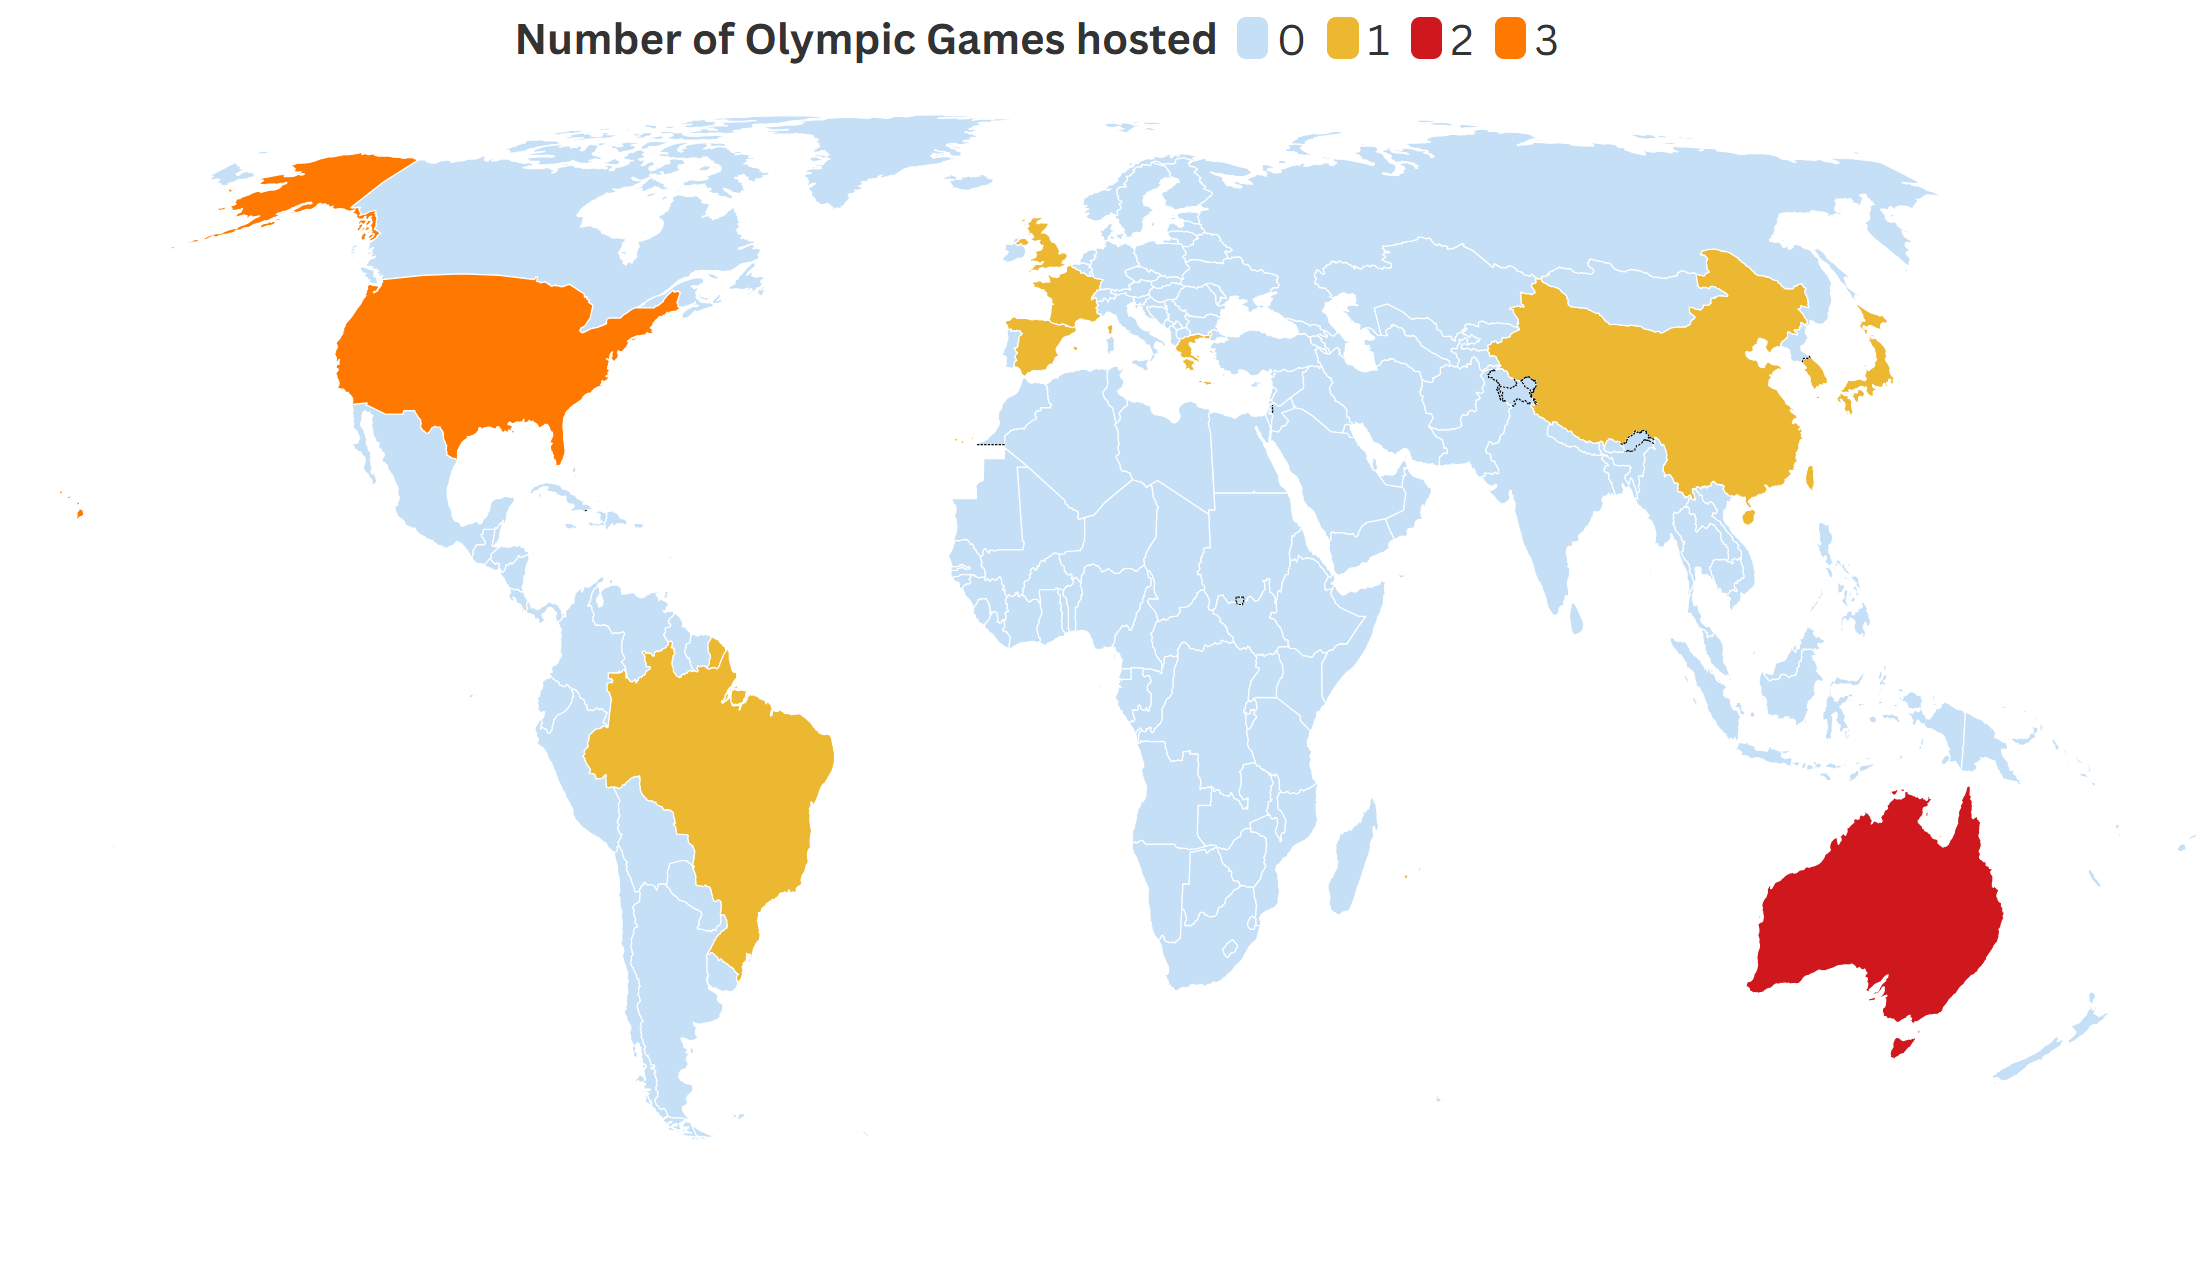
\includegraphics[width=\linewidth]{number_of_oly_hosted.png}
        \caption{Number of Olympic Games hosted}
        \label{fig:number_of_oly_hosted}
    \end{minipage}
\end{figure}

\subsection{Home Country Effect for Other Countries}
Our data shows a significant variation in the number of medals won by different countries from one session to the next. This indicates that it is largely due to the HC Effect, which impacts the host country as well as other ones. We have analysed the impact on countries with similar strong sports to the host country. The HC's unique weather, diet, sports pitch... can be extremely similar or vastly different to those in the athletes' native countries. This can lead to not adapting to the environment.Figure 23 shows the number of Olympics hosted after 1984.

The Olympic Committee should ensure that the HC are diverse and balanced in terms of factors like time zones, size, climate, so that the overall performance of each country is stable.

Furthermore, there are also factors like 2020 Japan (influenced by Covid-19), 2024 France (Russia cannot participate due to the political issue) that cannot be predicted. They are also important points that remain for the Olympic Committee to consider about. In our opinion, the first and only criteria is to remain JUSTICE and only consider the welfare of mankind.

\section{Final Prediction}

Our prediction is produced not only from our Core Medal Prediction Model, but also from the patches we designed to boost the accuracy and robustness of the model. After combining the results of both, along with the corresponding weighting and function compositing, the data shown in Figure 23 was obtained.

The first figure shows the overall predicted ranking of the countries below. It is summarized from the early years' results that three classes can be separated (ranking 1-2, 3-10, 11-15), and our prediction tend to follow this pattern.

The second figure shows the predicted Gold, Silver, Bronze, Total medal counts of the top 15th countries. The Gold and Total count is ranked in the third and fourth figure, comparing with the situations of 2024.

We asked ChatGPT what are the possible events of the new sports in 2028, and searched the countries that are capable of these sports. Moreover, we take Home Country Effect's 0.16\% boost into account, and also calculated the effect for other countries. Finally, as a reference, we compared the data of 1996 and 1984, which also has the Home Country of America. We noticed that in those datasets, America gained a huge lead in the gold and total medal count, which is identical to our prediction, providing a 82\% similarity.

Gold Ranking: USA, CHN, GBR, JPN, KOR, GER, AUS, FRA, IRI, ITA, CUB, NED, ESP, PRK, JAM. Total Ranking: USA, CHN, GBR, JPN, GER, FRA, AUS, KOR, ITA, NED, ESP, IRI, CUB, PRK, JAM.

\begin{figure}[h!]
    \centering
    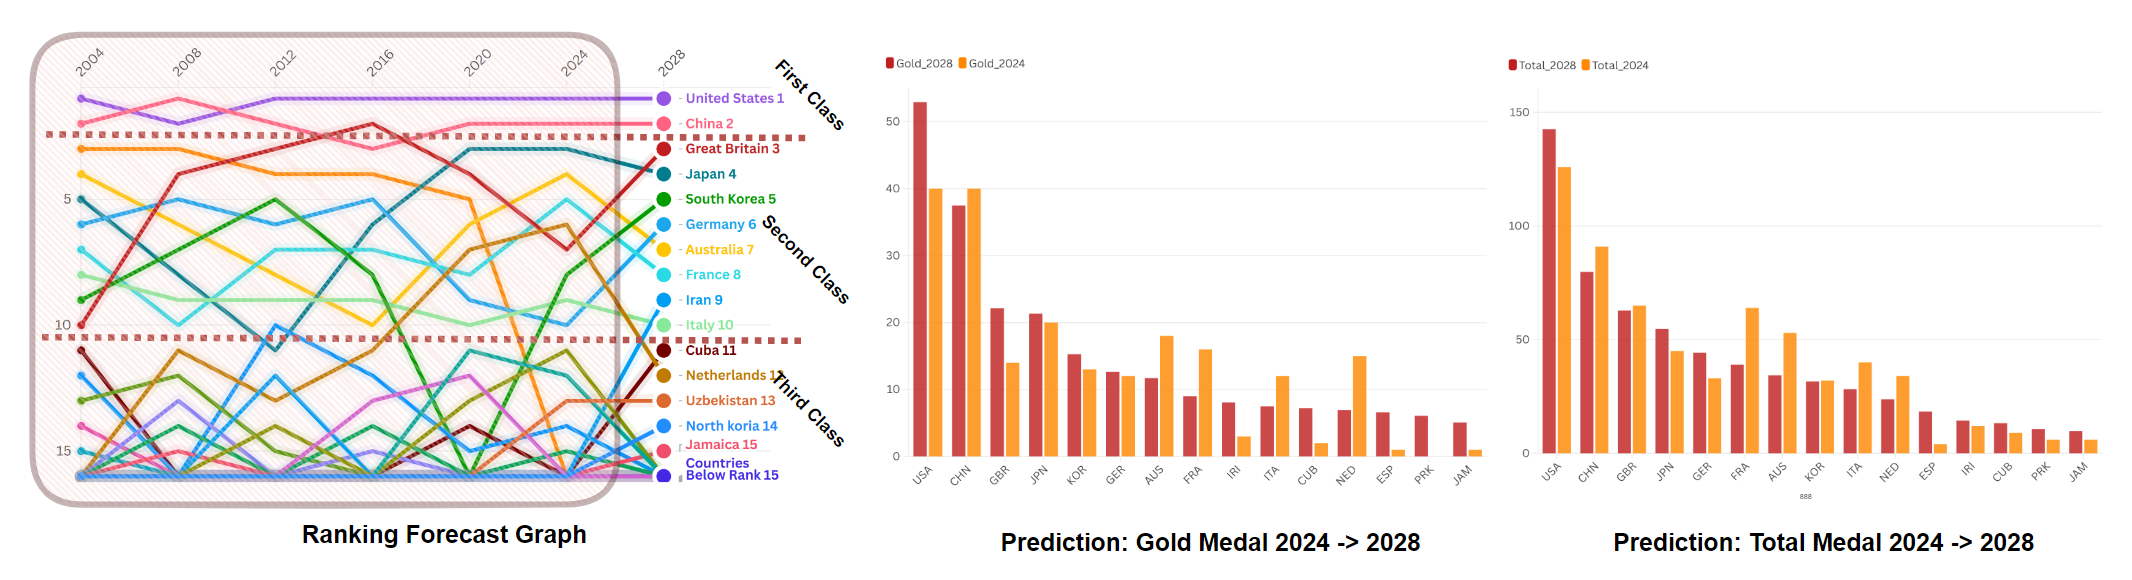
\includegraphics[width=1\textwidth]{Prediction.png}
    \caption{Our Final Prediction Graph Set}
    \label{fig:Prediction}
\end{figure}

\begin{table}[htbp]
\centering
\caption{2028 Predicted Medal Table}
\small
\begin{subtable}{0.48\textwidth}
\centering
\begin{tabular}{|c|c|c|c|c|}
\hline
\textbf{NOC} & \textbf{Gold} & \textbf{Silver} & \textbf{Bronze} & \textbf{Total} \\ \hline
\textbf{USA} & 52.92 & 49.63 & 40.13 & 142.7 \\ \hline
\textbf{CHN} & 37.48 & 19.42 & 22.94 & 79.84 \\ \hline
\textbf{GBR} & 22.13 & 21.07 & 19.64 & 62.83 \\ \hline
\textbf{JPN} & 21.34 & 11.41 & 21.98 & 54.73 \\ \hline
\textbf{KOR} & 15.28 & 4.960 & 11.41 & 31.64 \\ \hline
\textbf{GER} & 12.63 & 14.40 & 17.28 & 44.31 \\ \hline
\textbf{AUS} & 11.70 & 7.832 & 14.83 & 34.36 \\ \hline
\end{tabular}
\end{subtable}
\hfill
\begin{subtable}{0.48\textwidth}
\centering
\begin{tabular}{|c|c|c|c|c|}
\hline
\textbf{FRA} & 9.009 & 14.61 & 15.37 & 38.99 \\ \hline
\textbf{IRI} & 8.063 & 0.6879 & 5.685 & 14.44 \\ \hline
\textbf{ITA} & 7.485 & 7.353 & 13.40 & 28.23 \\ \hline
\textbf{CUB} & 7.227 & 2.270 & 3.758 & 13.25 \\ \hline
\textbf{NED} & 6.938 & 5.510 & 11.32 & 23.77 \\ \hline
\textbf{ESP} & 6.593 & 4.805 & 7.006 & 18.40 \\ \hline
\textbf{PRK} & 6.071 & 2.072 & 2.572 & 10.72 \\ \hline
\textbf{JAM} & 5.081 & 3.090 & 1.640 & 9.811 \\ \hline
\end{tabular}
\end{subtable}
\end{table}

% \subsection{Model Comparison}
% \label{sec:4.3}
% If we directly use ARIMA to predict the medal counts according to the past data, we found that the effect is far from great, which can be illustrated by Fig.~\ref{fig:arima_france} and Fig.~\ref{fig:arima-italy}. As shown in the results depicted in the image, when we directly apply the ARIMA model to historical medal datasets from Italy and France, The predicted results exhibit certain deviations from the actual outcomes, with a complete inconsistency in data trends.

% \begin{figure}
%     \centering
%         \begin{subfigure}[b]{0.49\textwidth}
%         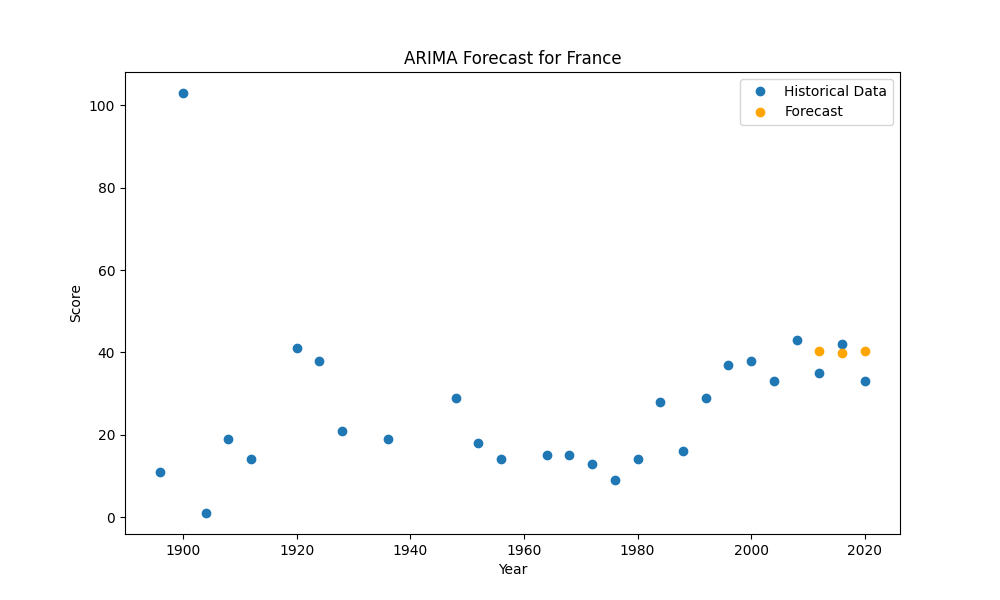
\includegraphics[width=\textwidth]{bad_france.png}
%         \caption{France's medal counts prediction}
%         \label{fig:arima_france}
%     \end{subfigure}
%     \hfill
%     \begin{subfigure}[b]{0.49\textwidth}
%         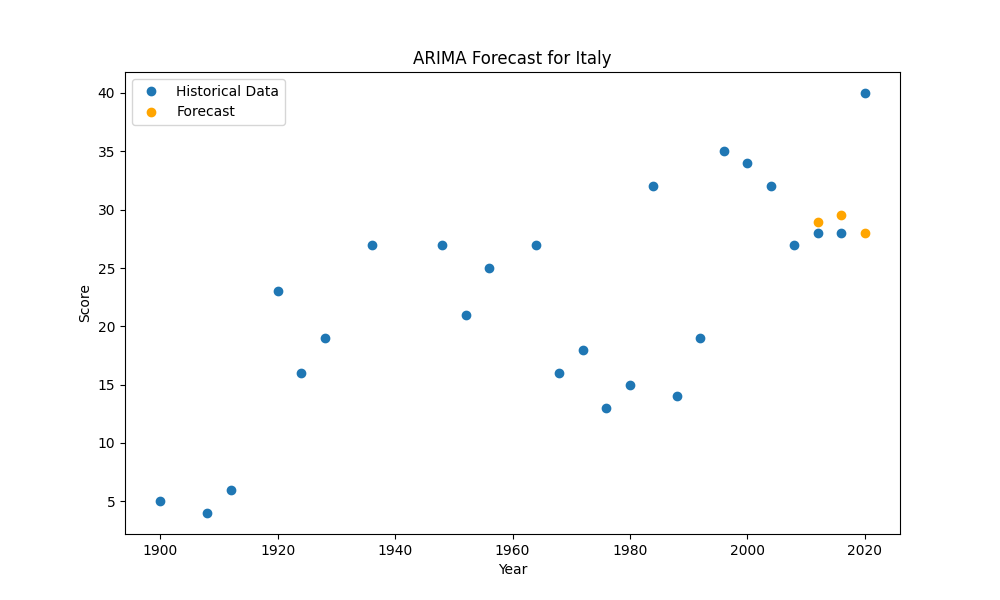
\includegraphics[width=\textwidth]{bad_italy.png}
%         \caption{Italy's medal counts prediction}
%         \label{fig:arima-italy}
%     \end{subfigure}
%     \caption{Directly use ARIMA to predict France's and Italy's medal counts.}
% \end{figure}

\section{Sensitivity Analysis}
\label{sec:9}
This sensitivity analysis aims to evaluate the impact of \textbf{hyperparameter variations} on the model’s performance and identify the most influential parameters. Since our model is very complicated and is comprised of several parts. We carried out sensitivity analysis for each part of the prediction model.

We found that these following parts are robust: Sport Gamma, $\Delta n$ predicition, veteran performance predicition. However, the recruit performance prediction is quite sensitive to parameter changes. The sensitivity of Sport Gamma to two important hyperparameters $\lambda_\alpha$ and $\lambda_\beta$ is illustrated by Fig~\ref{threed} and the sensitivity of a small perturbation of the Country / Sport GAMMA model parameters to the 2028 gold medal prediction for USA is illustrated by Fig~\ref{Pert}.

\begin{figure}[htbp]
    \centering
    \begin{minipage}{0.35\textwidth}
        \centering
        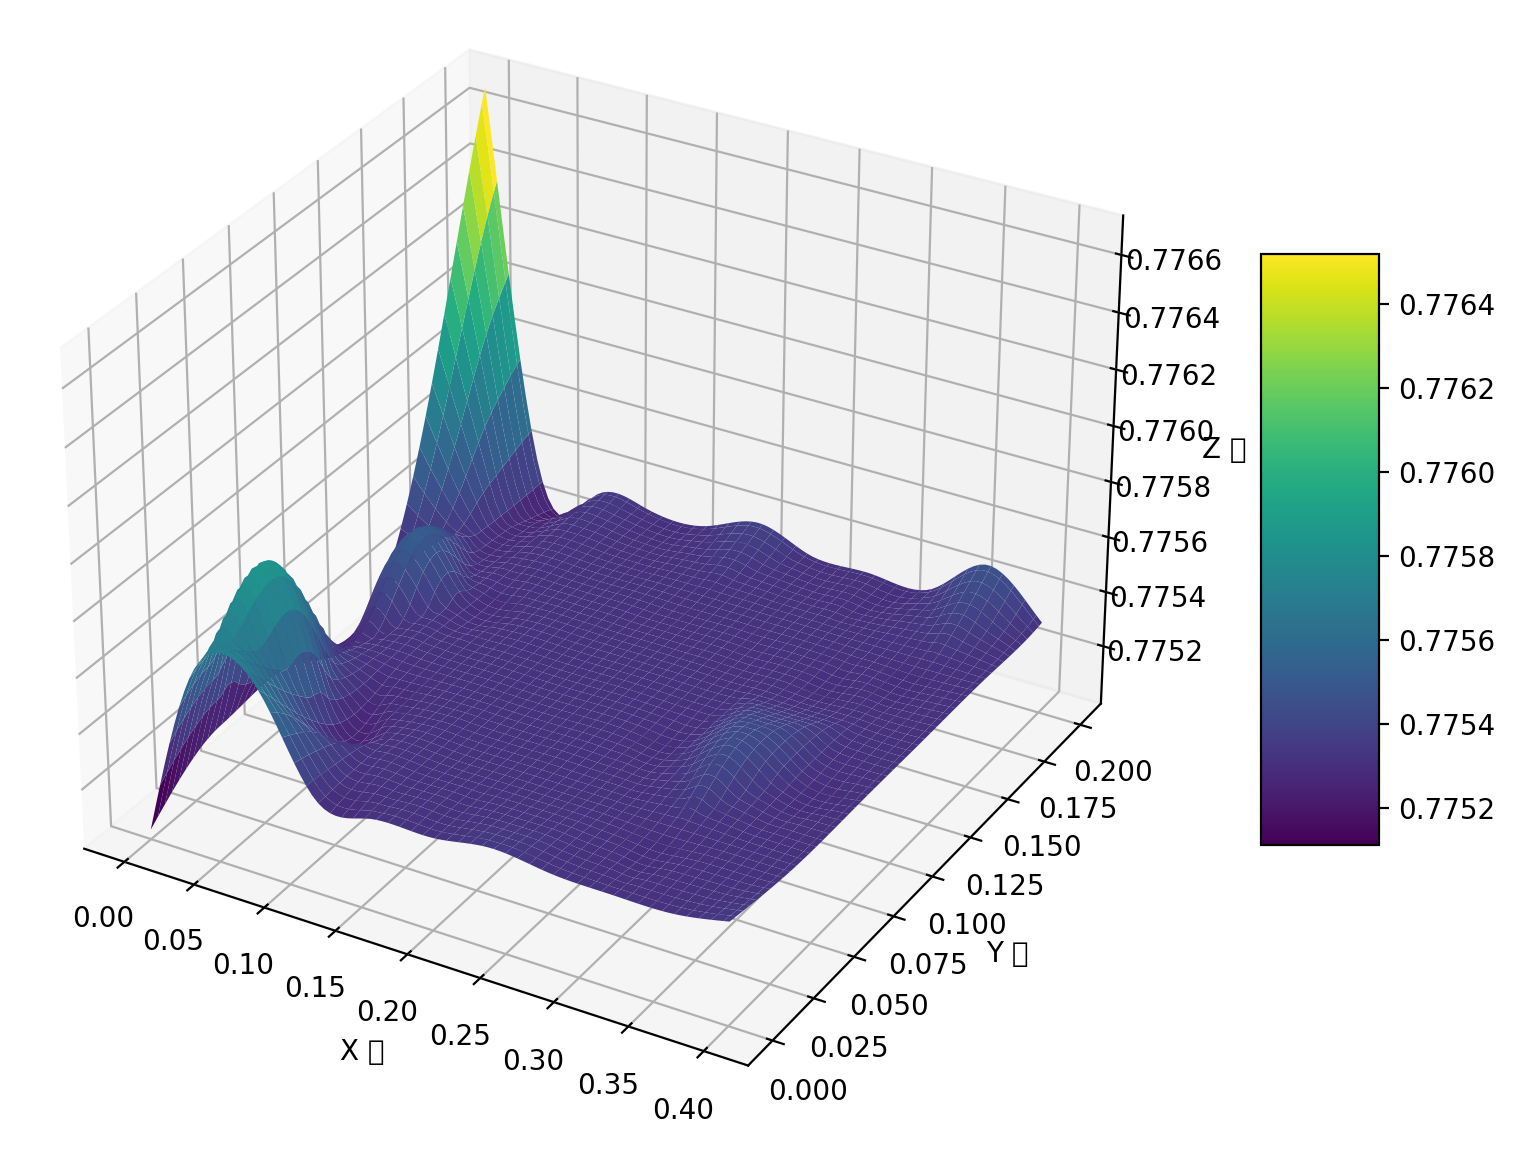
\includegraphics[width=\linewidth]{3d.png}
        \caption{Sensitivity of recruit performance prediction}
        \label{threed}
    \end{minipage}
    \hspace{0.05\textwidth} % 调整间距
    \begin{minipage}{0.35\textwidth}
        \centering
        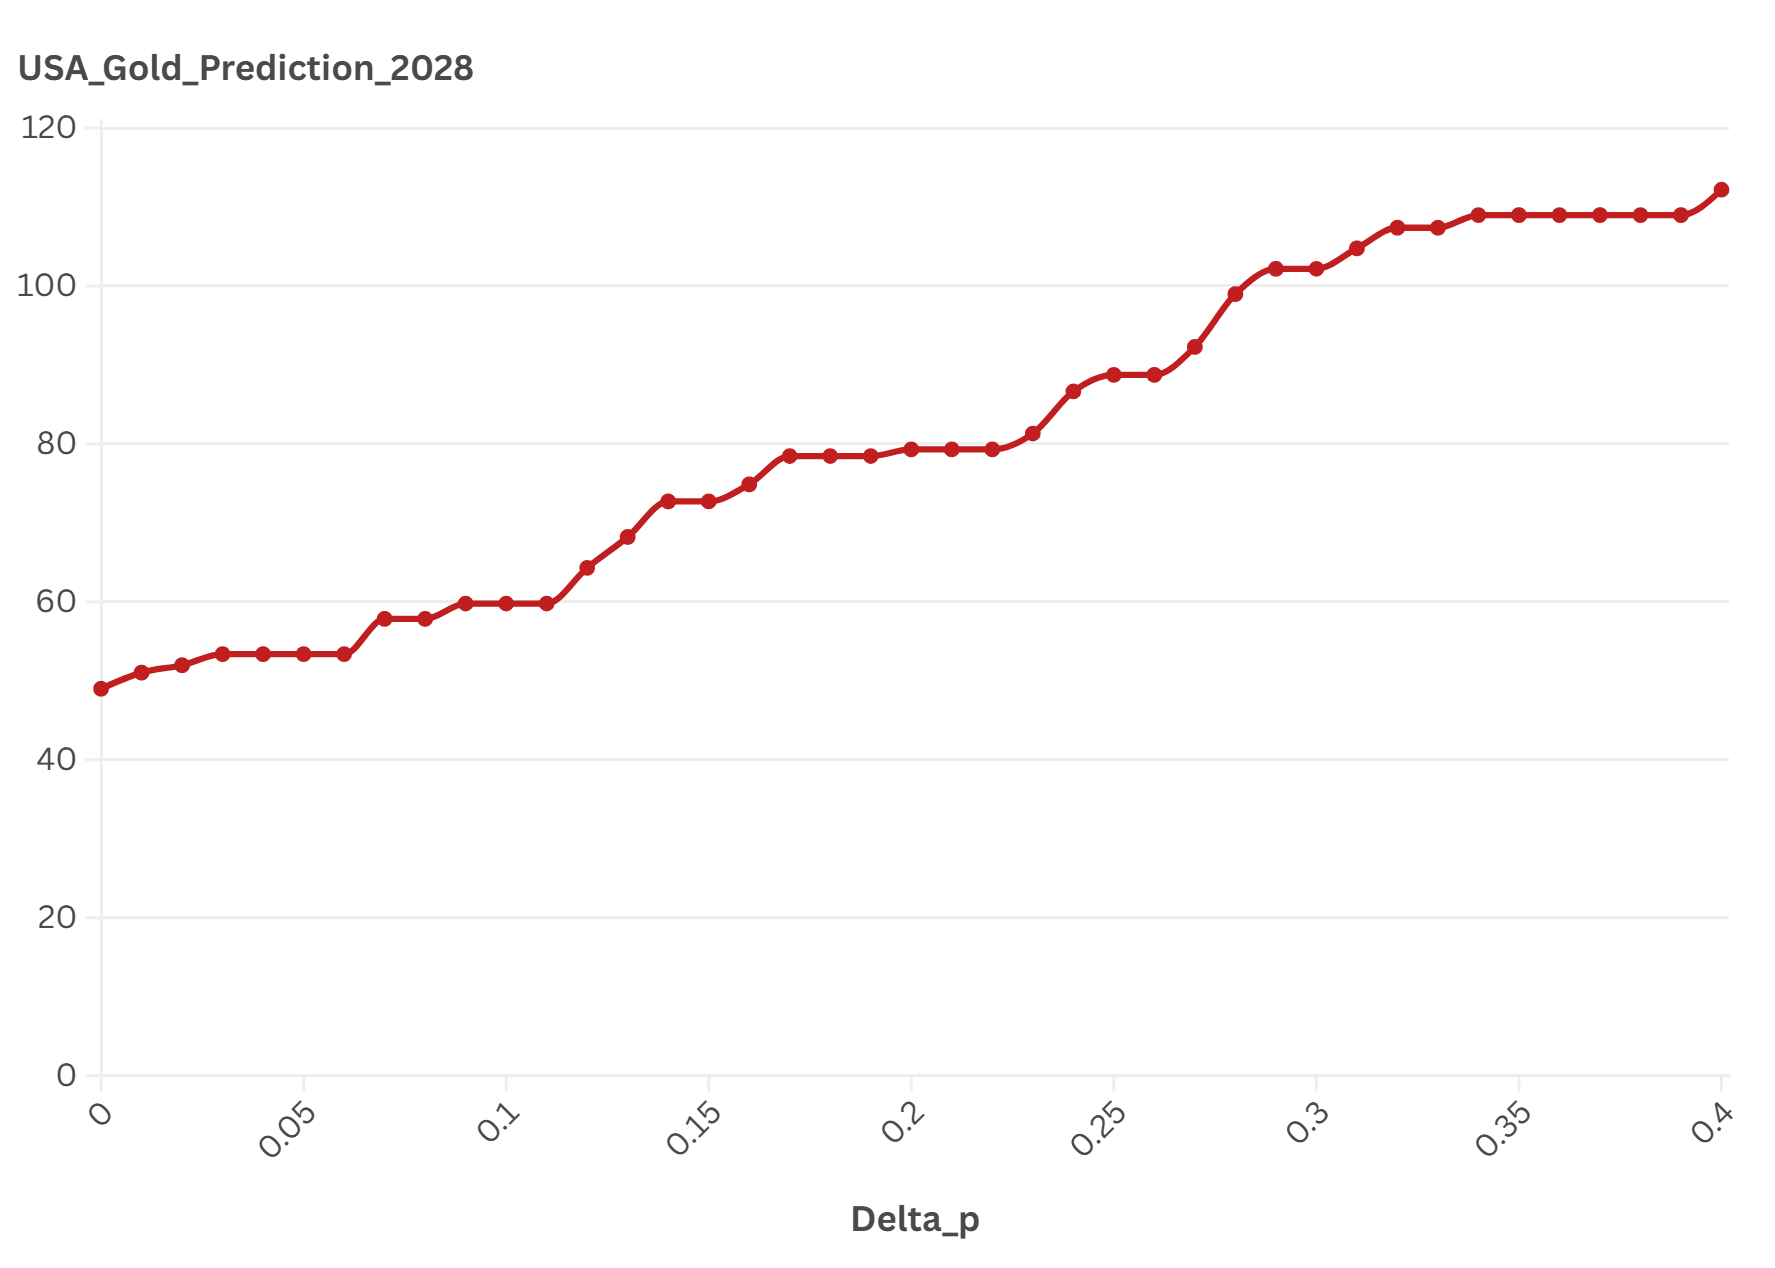
\includegraphics[width=\linewidth]{pert.jpg}
        \caption{Sensitivity of recruit performance prediction}
        \label{Pert}
    \end{minipage}
\end{figure}



\section{Conclusions}
\subsection{Strengths}

Our core model is not only a macroscopic model which has low interpretability and low accuracy, it also looks into each individual, which directly influences the medal counts. So our model is more accurate (especially for the veteran part) and has strong interpretabilities, so that we can gain insights by looking into the outliers. 

Besides, our model is not a single core model, but one with numerous of patches that explain and predict the large amount of seemingly 'outliers'. As is shown above, our core model itself only provides overall and rough prediction, while with the help of our various patch development, in cases like HC effect, Great Coach Effect, our comprehensive model can identify these potential effects and take them into account, refining and modifying our rough prediction, achieving a better performance.

\subsection{Weaknesses}
%主要由新兵决定,新兵的出现规律没有被很好的把握,考虑进去的因素较少。
The weakness of our model is mostly decided by these recruits, the regularity of whose appearance is not yet perfectly understood due to the limited number of factors considered. Additionally, as the data is so limited, the model parameters we simulated were, to a great extent, determined by random data and general laws. Furthermore, the simulation result is discrete, leading to a large deviation.
%由于可用数据极其少,拟合出来的模型参数很大程度上是由随机数据及一般规律决定,而且最后的拟合结果是离散结果,容易发生较大偏差

According to our model, the annual number of veterans per country is largely determined by the number of veterans in previous years, which is relatively rough as the improvement in the performance of athletes from 4 years ago could motivate the increase in veterans.
%我们的模型中,国家每年新增人数主要由国家前几年新增人数决定,略显粗略,因为其实上一届运动员的表现变好也能可能激励也会导致第二年新增人数增多。

In our patched models, some of the models require further data support in order to get a more precise result and prediction. For some other models, like the Great Coach Effect model, the overall system may be too simple that it cannot achieve an accuracy up to 90\%+, because some other effects may also act similarly to Great Coach Effect. This needs further research to find more factors. Moreover, the factors themselves may be unpredictable, which will always bring us some outliers. But that's the meaning of prediction - everything is possible.



\newpage

\begin{thebibliography}{99}
\addcontentsline{toc}{section}{Reference}

\bibitem{1} COMAP 2025. Problem C data set.2025
\bibitem{2} Griffin, J., Hinoveanu, L. , Hopker J. (2022). Bayesian modelling of elite sporting performance with large databases. Journal of Quantitative Analysis in Sports, 18(4), 253-268.
\bibitem{3} Olympics.com Biography, Lang Ping, \url{https://olympics.com/en/athletes/ping-lang}
\bibitem{4} USA Gymnastics Hall of Fame,
\url{https://usagym.org/halloffame/inductee/coaching-team-bela-martha-karolyi/}
\bibitem{5} Cox,D.R., Prediction by Exponentially Weighted Moving Averages and Related Methods. Journal of the Royal Statistical Society: Series B (Methodological), 23: 414-422 (1961).
\bibitem{6} James M. Lucas , Michael S. Saccucci , Exponentially Weighted Moving Average Control Schemes: Properties and Enhancements, Technometrics, 32:1, 1-12 (1990)
\bibitem{7} Box, G.E., Jenkins, G.M., Reinsel, G.C., \& Ljung, G.M. (1978). Time Series Analysis: Forecasting and Control. The Statistician, 27, 265-265.
\bibitem{8} Hotelling, H. (1933). Analysis of a complex of statistical variables into principal components. Journal of Educational Psychology, 24, 498-520.
\bibitem{9} Bian, Xun. (2005). Predicting Olympic Medal Counts: the Effects of Economic Development on Olympic Performance. Honors Projects. 13. 
\bibitem{10} Wikipedia.org, Sarah Kolak,\url{https://en.wikipedia.org/wiki/Sara_Kolak}

\end{thebibliography}

\newpage

\begin{appendices}
\section{Modeling Details}
\label{appA}


\begin{tabular}{|p{1cm}|p{3cm}|p{10cm}|}
\hline
\textbf{Sec.} & \textbf{Theme} & \textbf{Activity} \\
\hline
4.1 & Team event & %We query GPT to filter all team events. We then rewrote the data-processing code to clean the dataset and obtain the actual number of participants for each team event, adding a new column  file. When predicting the number of participants, no changes are required, but when calculating the loss for the predicted number of participants, it needs to be divided by the number of participants in the team event. The same division by this number applies when predicting the medal count. 
We queried GPT to filter team events, cleaned the dataset, and added a column in the {\texttt{summerOly\_athletes.csv}} for the actual number of participants per team event. For participant number prediction, no changes are needed, but calculating the loss requires dividing by the number of participants, which also applies to medal count predictions.\\
\hline
5.1 & The strategy of filling missing value for Country / Sport Gamma distribution time series prediction. & When performing time series prediction for the country’s Gamma distribution, for default data, in order to ensure data completeness, we didn't fill in the default value. Instead, we designed the following algorithm. (The pseudocode used for data processing is in algorithm~\ref{alg_F,M,V}.) This approach is used because the strength of the athletes produced by the country has not changed, and the missing data is due to various reasons such as specific events not being included in the competition that year. Comparing with simply setting all parameters to 0, this approach is more intuitive.  \\
\hline
5.3 & The possibilites of veterans participating in the next game. & If the \( p \) for a sport is greater than the \( p \) from training without distinguishing the sport, use the sport's own \( p \); if it's smaller, use the \( p \) from the training without distinguishing the sport (however, we avoid sports with limited data, such as breaking, where the \( p \) is NAN).
 \\
\hline
\end{tabular}



%\textbf{\textcolor[rgb]{0.98,0.00,0.00}{Input pseudocode source:}}
%\lstinputlisting[basicstyle=\scriptsize]{./code/Gammacode.txt}
\begin{algorithm}[H]
    \caption{Fill Missing Values}
    \label{alg_F,M,V}
    \BlankLine
    $\text{default\_values} = \big\{ 
        \text{p\_max} \mapsto 0.5,\ 
        \text{a\_max} \mapsto 5,\ 
        \text{alpha} \mapsto 0.2,\ 
        \text{beta} \mapsto 0.05 
        \big\}$\;
    \For{$i$ from 0 to $\text{length}(merged\_df) - 1$}{
        \If{$\text{merged\_df.loc}[i, \text{'p\_max'}]$ is NaN}{
            \If{$i > 0$ and $\text{merged\_df.loc}[i - 1, \text{'p\_max'}] \neq \text{default\_values}[\text{'p\_max'}]$}{
                $\text{merged\_df.loc}[i, \text{'p\_max'}] = \text{merged\_df.loc}[i - 1, \text{'p\_max'}] \times 0.9$\;
                $\text{merged\_df.loc}[i, \text{'a\_max'}] = \text{merged\_df.loc}[i - 1, \text{'a\_max'}]$\;
                $\text{merged\_df.loc}[i, \text{'alpha'}] = \text{merged\_df.loc}[i - 1, \text{'alpha'}]$\;
                $\text{merged\_df.loc}[i, \text{'beta'}] = \text{merged\_df.loc}[i - 1, \text{'beta'}]$\;
            }
            \Else{
                $\text{merged\_df.loc}[i, \text{'p\_max'}] = \text{default\_values}[\text{'p\_max'}]$\;
                $\text{merged\_df.loc}[i, \text{'a\_max'}] = \text{default\_values}[\text{'a\_max'}]$\;
                $\text{merged\_df.loc}[i, \text{'alpha'}] = \text{default\_values}[\text{'alpha'}]$\;
                $\text{merged\_df.loc}[i, \text{'beta'}] = \text{default\_values}[\text{'beta'}]$\;
            }
        }
    }
    \Return{merged\_df}\;
\end{algorithm}

\section{The derivation of Bayes’ theorem.}
\label{appB}
The meanings of the notations are already explained above. Here are the concrete derivation.
\begin{align*}
    p(s \mid pre, c)  &= \frac{p(pre, c \mid s) \cdot p(s)}{p(pre, c)} \\[10pt]
    p(s \mid pre) &= \frac{p(pre \mid s) \cdot p(s)}{p(pre)} \\[10pt]
    \frac{p(s \mid pre, c)}{p(s \mid pre)} &= \frac{\frac{p(pre, c \mid s) \cdot p(s)}{p(pre, c)}}{\frac{p(a \mid s) \cdot p(s)}{p(pre)}} \\[10pt]
    &= \frac{p(pre, c \mid s) \cdot p(pre)}{p(pre, c) \cdot p(pre \mid s)}
\end{align*}
According to above analysis, we have:
\begin{itemize}
    \item \textbf{pre} and \textbf{c} are conditionally independent given \textbf{s}:
    \[
    p(pre, c \mid s) = p(pre \mid s) \cdot p(c \mid s).
    \]
    \item \textbf{pre} and \textbf{c} are independent in the absence of conditions:
    \[
    p(pre, c) = p(pre) \cdot p(c).
    \]
\end{itemize}

Under these conditions:
\[
\frac{p(s \mid pre, c)}{p(s \mid pre)} = \frac{p(pre \mid s) \cdot p(c \mid s) \cdot p(pre)}{p(pre) \cdot p(c) \cdot p(pre \mid s)} = \frac{p(c \mid s)}{p(c)}.
\]

According to Bayes' theorem:
\[
\frac{p(c \mid s)}{p(c)} = \frac{p(s \mid c)}{p(s)}.
\]

Thus, under the conditions of independence and conditional independence between \textbf{pre} and \textbf{c}, the equation holds:
\[
p(s \mid pre, c) = \frac{p(s \mid c) \cdot p(s \mid pre)}{p(s)}.
\]

\end{appendices}

\newpage
\newcounter{lastpage}
\setcounter{lastpage}{\value{page}}
\thispagestyle{empty} 

\section*{Report on Use of AI}

\begin{enumerate}
\item OpenAI ChatGPT (Nov 5, 2023 version, ChatGPT-4) 
\begin{description}
\item[Query1:] (1) Swimming Athletics Basketball Equestrian\\
(2) Weightlifting Badminton Artistic swimming Wrestling\\
(3) Badminton Table Tennis Artistic swimming Cycling Track\\
(4) Skateboarding Softball Baseball Beach Volleyball\\
Please summarize the common characteristics of each row, which should be distinctive and highly representative. 
\item[Output:] I understand that you want to identify a distinctive and representative common characteristic for each row. We can find the most representative feature based on the nature of the sports in each row. Here is the summary for each row:\\
Row 1: Swimming, Athletics, Basketball, Equestrian\\
Common Feature: "Traditional and Classic Competitive Sports"\\
These sports are classic competitive events with a long history and widespread participation, often featured in major international competitions like the Olympics. They are highly competitive and attract a diverse range of countries and regions, drawing a broad global audience.\\
Row 2: Weightlifting, Badminton, Artistic Swimming, Wrestling\\
Common Feature: "Sports Highly Dependent on Technique and Skill"\\
The sports in this row emphasize the athlete's technique, skill, and precision. Whether it's the technical movements in weightlifting, the skillful strokes in badminton, the coordination in artistic swimming, or the tactical skills in wrestling, all these sports rely not only on strength but more on skill and precise movement control.\\
Row 3: Badminton, Table Tennis, Artistic Swimming, Cycling Track\\
Common Feature: "Sports Emphasizing Quick Reactions and Precise Control"\\
The common feature of these sports is the high demand for reaction speed and precise control. Badminton, table tennis, and artistic swimming all require extremely fast reactions and fine motor coordination, while track cycling demands precise control over the trajectory of movement, emphasizing quick reactions and precise control abilities.\\
Row 4: Skateboarding, Softball, Baseball, Beach Volleyball\\
Common Feature: "Modern and Highly Visually Appealing Sports"\\
These sports have a strong modern feel and high visual appeal. Skateboarding, beach volleyball, and baseball (especially with baseball's recent return to the Olympics) are popular among young people and have a strong visual impact. Particularly skateboarding has become a focus of street culture and Olympic competition, offering strong entertainment and visual appeal.\\
Summary:\\
Row 1: "Traditional and Classic Competitive Sports"\\
Row 2: "Sports Highly Dependent on Technique and Skill"\\
Row 3: "Sports Emphasizing Quick Reactions and Precise Control"\\
Row 4: "Modern and Highly Visually Appealing Sports"\\
Each common feature highlights the core attributes of the sports in that row and is distinctive and unique, providing a good summary of the type of sports in each row. If you have any other specific requirements, feel free to let me know!\\

\item[Query2:] Help me create a dictionary, mapping all the countries to NOC.
\item[Output:] Here is a Python dictionary that maps countries to their respective NOCs (National Olympic Committees):
country\_to\_NOC = \{ \\
"United States": "USA",\\
"Great Britain": "GBR",\\
"China": "CHN",\\
"Russia": "RUS",\\
"Germany": "GER",\\
"Japan": "JPN",\\
"France": "FRA",\\
"South Korea": "KOR",\\
"Italy": "ITA",\\
"Australia": "AUS",\\
"Netherlands": "NED",\\
"Hungary": "HUN",\\
"Brazil": "BRA",\\
"Spain": "ESP",\\
"Kenya": "KEN",\\
"Jamaica": "JAM",\\
"Croatia": "CRO",\\
"Cuba": "CUB",\\
"New Zealand": "NZL",\\
"Canada": "CAN",\\
"Uzbekistan": "UZB",\\
"Colombia": "COL",\\
"Switzerland": "SUI",\\
"Iran": "IRI",\\
"Greece": "GRE",\\
"Argentina": "ARG",\\
"Denmark": "DEN",\\
"Sweden": "SWE",\\
"South Africa": "RSA",\\
"Kazakhstan": "KAZ",\\
"Ukraine": "UKR",\\
"Serbia": "SRB",\\
"Poland": "POL",\\
"North Korea": "PRK",\\
"Belgium": "BEL",\\
"Thailand": "THA",\\
"Slovakia": "SVK",\\
"Georgia": "GEO",\\
"Azerbaijan": "AZE",\\
"Belarus": "BLR",\\
"Turkey": "TUR",\\
"Armenia": "ARM",\\
"Czech Republic": "CZE",\\
"Ethiopia": "ETH",\\
"Slovenia": "SLO",\\
"Indonesia": "INA",\\
"Romania": "ROU",\\
"Bahrain": "BRN",\\
"Vietnam": "VIE",\\
"Chinese Taipei": "TPE",\\
"Bahamas": "BAH",\\
"Independent Olympic Athletes": "IOA",\\
"Ivory Coast": "CIV",\\
"Fiji": "FIJ",\\
"Jordan": "JOR",\\
"Kosovo": "KOS",\\
"Puerto Rico": "PUR",\\
"Singapore": "SGP",\\
"Tajikistan": "TJK",\\
"Malaysia": "MAS",\\
"Mexico": "MEX",\\
"Venezuela": "VEN",\\
"Algeria": "ALG",\\
"Ireland": "IRL"\\
\}

\item[Query3:] What are the possible events that may occur in 2028 Summer Olympics, according to the added sports list: Baseball/softball, cricket, flag football, lacrosse, squash?
\item[Output:]Projected breakdown of programs:\\
1. Baseball/Softball\\
Baseball: Major League Baseball (MLB): the standard professional baseball league, primarily distinguished from other levels of the game in terms of player strength, pace of play, and athletic demands.\\
Fast Pitch Baseball (Fast Pitch) and Slow Pitch Baseball (Slow Pitch): These are the two main types of baseball and softball pitching, with Slow Pitch being more commonly seen in recreational and women's games, and Fast Pitch being more commonly used in professional games.\\
Softball: Fast Pitch Softball: The game is faster and the rules are closer to those of baseball.\\
Slow Pitch Softball: A slow pitch with a curved path that requires a high degree of skill and strategy.\\
Wall Softball: Using multi-angle wall bounce to increase the difficulty, more competitive.\\
2. Cricket\\
International Cricket (International Cricket): such as One Day International (ODI), Twenty20 (T20), etc., is currently the most popular form of cricket around the world.\\
Test Cricket: A traditional cricket match that lasts five days and emphasizes endurance and strategy.\\
Ten-a-Side Cricket: Reduced to 10 players per team, the game is faster paced.\\
Street Cricket: Informal form of cricket, commonly played on city streets, backyards, etc.\\
3. Flag Football\\
Men's/Women's Flag Football: divided into men's and women's games, the rules are less different, mainly in the physical ability of the participants, speed.\\
7-a-side Flag Football: Compared to traditional 11-a-side football, the field and personnel are smaller, and the game is more tactically oriented.\\
Mixed Sex Flag Rugby: A format in which both men and women play together, with rules adjusted for physical demands and an emphasis on tactical cooperation.\\
4. Lacrosse\\
Men's Lacrosse: In contrast to Women's Lacrosse, Men's Lacrosse is more physically demanding and utilizes hard protective equipment.\\
Women's Lacrosse: The rules are relatively mild and emphasize skill and speed.\\
Box Lacrosse: Played on closed courts, the game is faster paced and more physical, and is commonly played in Canada.\\
Field Lacrosse: Unlike indoor lacrosse, it is usually played on a large grass field and the pace of the game is relatively slow.\\
5. Squash\\
Singles Squash: Two players play against each other using singles rules.\\
Doubles Squash (Doubles Squash): four players participate in the game, the rules of the game is similar to the singles, but there is more movement and cooperation on the court.\\
Soft Squash: A softer ball, suitable for beginners or older players.\\
Hardball Squash: A more challenging game using hard balls, commonly played in the United States.\\


\item[Query4:]
Help me identify all the team sports listed below:\\
B-Girls\\
Women's Sabre Individual\\
Men's 67kg\\
Jumping Individual\\
Women's 200m Freestyle\\
Basketball Men's Basketball\\
Judo Men's Extra-Lightweight\\
Women's +87kg\\
Football Men's Football\\
Athletics Men's Long Jump\\
...
\item[Output:] Here is the identification of team sports from the list provided:

Team Sports:
	1.	Basketball Men’s Basketball – Team sport\\
	2.	Football Men’s Football – Team sport\\
	3.	Hockey Men’s Hockey – Team sport\\
 ...


 
\end{description}

\item DeepL (Version 25.1.4.15077+495e4eb7b7cc47c7c43de87ac335c76ea3e6a019)
\begin{description}
\item We used it as a translator for some special nouns and words we do not know.
 
\end{description}
\end{enumerate}

% 重置页码
\clearpage
\setcounter{page}{\value{lastpage}}

\end{document}
%%
%% This work consists of these files mcmthesis.dtx,
%%                                   figures/ and
%%                                   code/,
%% and the derived files             mcmthesis.cls,
%%                                   mcmthesis-demo.tex,
%%                                   README,
%%                                   LICENSE,
%%                                   mcmthesis.pdf and
%%                                   mcmthesis-demo.pdf.
%%
%% End of file `mcmthesis-demo.tex'.
